% ============================================================
% Master's Thesis - main document
% Deggendorf Institute of Technology (DIT)
%
% Compiles with the default "pdfLaTeX" recipe (Overleaf: Menu ->
% Compiler -> pdfLaTeX). Bibliography uses plain BibTeX, not
% biblatex/biber - deliberately, to keep the compile chain short
% enough for Overleaf's free-tier compile-time limit:
%   pdflatex -> bibtex -> pdflatex -> pdflatex
% Overleaf detects and runs this chain automatically; no manual step
% needed beyond a normal Recompile.
%
% TODO (you): fill in every "TODO" marker across this project before
% submission - title page fields, abstract, acknowledgement, and the
% content TODOs left inside each chapter file.
% ============================================================

\documentclass[11pt,a4paper,oneside]{report}

% ============================================================
% Preamble: formatting compliance with the DIT Thesis Guideline
% (Deggendorf Institute of Technology, "Thesis Guideline",
%  Version 1.0, 27.06.2023)
%
% Requirements implemented here:
%  - DIN A4, single-sided printing
%  - Font size 11-12pt body, 14pt chapter headings
%  - Margins: top 2.5cm, bottom 2.5cm, left 3cm, right 2cm
%  - 1.5 line spacing
%  - Justified text with automatic hyphenation
%  - Consecutive page numbers in header/footer
%  - Section numbering 1, 1.1, 1.2, 2, 2.1, 2.1.1 ...
%  - Headings: not underlined/indented, bold, same font as body,
%    start with capital letter, fit on one line
%  - No university logo anywhere (guideline 4.1.1 / 3.5)
% ============================================================

% --- Page geometry -------------------------------------------------
\usepackage[a4paper,top=2.5cm,bottom=2.5cm,left=3cm,right=2cm]{geometry}

% --- Language / hyphenation -----------------------------------------
% Switch babel's main language to ngerman if you write in German;
% keep english if the thesis is written in English (check with your
% supervisor which language is expected).
\usepackage[english]{babel}
\usepackage[utf8]{inputenc}
\usepackage[T1]{fontenc}

% Latin Modern: a fully scalable (outline) replacement for the default
% Computer Modern fonts. Needed because titlesec below requests
% non-standard font sizes (e.g. \fontsize{14}{16} for chapter
% headings); without lmodern, LaTeX falls back to Metafont-generated
% bitmap fonts at those sizes, which are not scalable - and microtype's
% font expansion feature then fails with a fatal
% "auto expansion is only possible with scalable fonts" error.
\usepackage{lmodern}

% --- Font size (11-12pt body, set via documentclass option) --------
% Body font size is set as a \documentclass option in main.tex.

% --- Line spacing: 1.5 -----------------------------------------------
\usepackage{setspace}
\onehalfspacing

% --- Justification with automatic hyphenation ------------------------
% LaTeX justifies by default; microtype improves justification quality
% (fewer visible stretched/compressed lines) without changing the
% guideline-required "justification with automatic hyphenation" look.
\usepackage{microtype}

% This thesis's prose is dense with long, non-hyphenating \texttt{}
% identifiers (ROS topic/plugin/parameter names). Without headroom,
% TeX sometimes has no legal break short of pushing text past the
% right margin ("Overfull \hbox"), which would visibly violate the
% guideline's "illustrations and tables [text] are to remain within
% the page margins" requirement. emergencystretch gives the
% line-breaker extra last-resort stretch before it would otherwise
% overfull, fixing these without loosening ordinary paragraphs.
\emergencystretch=3em

% A handful of table cells hold long filename-like identifiers
% (e.g. libgazebo_ros_ackermann_drive.so) that are still wider than
% their column even with emergencystretch, since that only adds
% inter-word stretch and these are single unbreakable "words". seqsplit
% allows breaking such a token at any character as a last resort, kept
% to just those specific cells rather than used document-wide.
\usepackage{seqsplit}

% --- Headings: bold, same font as body text, not underlined ----------
\usepackage{titlesec}
\titleformat{\chapter}[hang]
  {\normalfont\fontsize{14}{16}\bfseries}{\thechapter}{1em}{}
\titleformat{\section}
  {\normalfont\fontsize{12}{14}\bfseries}{\thesection}{1em}{}
\titleformat{\subsection}
  {\normalfont\fontsize{11}{13}\bfseries}{\thesubsection}{1em}{}
\titleformat{\subsubsection}
  {\normalfont\fontsize{11}{13}\bfseries}{\thesubsubsection}{1em}{}
\titlespacing*{\chapter}{0pt}{0pt}{20pt}

% --- Section numbering depth (down to subsubsection, e.g. 2.1.1) -----
\setcounter{secnumdepth}{3}
\setcounter{tocdepth}{3}

% --- Footnotes: numbered consecutively throughout the document, not
% reset per chapter (mandatory per the Campus Cham "Specific
% Instructions" registration document) -----------------------------
\usepackage{chngcntr}
\counterwithout{footnote}{chapter}

% --- Header/footer: consecutive page numbers --------------------------
\usepackage{fancyhdr}
\pagestyle{fancy}
\fancyhf{}
\fancyfoot[C]{\thepage}
\renewcommand{\headrulewidth}{0pt}

% A plain style for chapter-opening pages (still numbered, no header rule)
\fancypagestyle{plain}{
  \fancyhf{}
  \fancyfoot[C]{\thepage}
  \renewcommand{\headrulewidth}{0pt}
}

% --- Figures and tables ------------------------------------------------
\usepackage{graphicx}
\usepackage{caption}
\usepackage{subcaption}
\captionsetup{font=small,labelfont=bf,justification=justified}
\usepackage{booktabs}   % clean table rules (no vertical/frame lines)
\usepackage{longtable}  % tables that span multiple pages (Results ch.)
\usepackage{array}

% --- Diagrams and plots -------------------------------------------------
% No photos/screenshots exist for this thesis; every figure is instead
% drawn directly from data and mechanisms already described in the
% prose (architecture block diagrams, a path-geometry diagram, and
% pgfplots charts built from the thesis's own result tables), so a
% reader never has to take a described mechanism or number on faith.
\usepackage{tikz}
\usetikzlibrary{arrows.meta,positioning,calc,fit,backgrounds}
\usepackage{pgfplots}
\pgfplotsset{compat=1.17}

% --- Formulas and physical quantities -----------------------------------
\usepackage{amsmath}
\usepackage{amssymb}
\usepackage{siunitx}    % correct unit typesetting: \SI{2.3}{\ampere} etc.
\sisetup{
  detect-all,
  output-decimal-marker = {.},   % dot as decimal separator (English)
  per-mode = symbol
}

% --- Code / configuration listings (launch files, YAML, Python) --------
\usepackage{listings}
\usepackage{xcolor}
\definecolor{codebg}{RGB}{245,245,245}

% Custom, minimal language definitions for every language= used in this
% thesis's lstlisting blocks (Python, C++, XML, bash), defined BEFORE
% any \begin{lstlisting} uses them. This deliberately overrides
% `listings`'s own bundled per-language keyword databases
% (lstlang1.sty/lstlang2.sty/lstlang3.sty) rather than relying on them -
% a known TeX Live 2026 regression in that bundled data triggers
% "Extra alignment tab has been changed to \cr" from inside
% lstlang1.sty on some language definitions. Defining the language
% ourselves means `listings` never loads the bundled file for these
% four names at all, sidestepping the bug regardless of exactly which
% bundled definition is at fault. Highlighting is intentionally simple
% (comments, strings, a short keyword list) - plenty for short
% illustrative snippets, and it will never break a compile this way.
\lstdefinelanguage{Python}{
  morekeywords={def,class,if,elif,else,for,while,return,import,from,as,
    try,except,finally,with,lambda,None,True,False,and,or,not,in,is,
    break,continue,pass,raise,yield,global,nonlocal,self,print},
  sensitive=true,
  morecomment=[l]{\#},
  morestring=[b]",
  morestring=[b]'
}
\lstdefinelanguage{XML}{
  morecomment=[s]{<!--}{-->},
  morestring=[b]",
  morestring=[b]',
  sensitive=true
}
\lstdefinelanguage{C++}{
  morekeywords={void,int,float,double,bool,char,const,static,class,
    struct,namespace,public,private,protected,return,if,else,for,
    while,do,switch,case,break,continue,new,delete,template,typename,
    using,auto,size_t,true,false,nullptr,enum},
  sensitive=true,
  morecomment=[l]{//},
  morecomment=[s]{/*}{*/},
  morestring=[b]"
}
\lstdefinelanguage{bash}{
  morekeywords={sudo,python3,ros2,run,launch,env,export,echo,cd},
  sensitive=true,
  morecomment=[l]{\#},
  morestring=[b]",
  morestring=[b]'
}

\lstset{
  basicstyle=\ttfamily\small,
  backgroundcolor=\color{codebg},
  breaklines=true,
  frame=single,
  framerule=0.3pt,
  columns=flexible,
  captionpos=b,
  numbers=left,
  numberstyle=\tiny,
  keywordstyle=\color{blue!60!black}\bfseries,
  commentstyle=\color{gray},
  showstringspaces=false
}

% --- Bibliography: numeric, DIN-style [1]-style in-text citation -------
% Plain LaTeX + BibTeX (\bibliographystyle{plain} in main.tex), not
% biblatex/biber: functionally equivalent numeric-bracket output for a
% bibliography this size, but only one extra compile pass instead of
% biber's own (slower) separate backend - matters on Overleaf's free
% compile-time limit. \bibliographystyle{plain} already sorts entries
% alphabetically by author while numbering them [1], [2], ... in that
% order, matching the guideline's "numbered upon citation order OR
% alphabetically sorted" allowance (here: both at once).

% --- Abbreviations list --------------------------------------------------
% Rendered as a plain table (frontmatter/abbreviations.tex) rather than
% via the glossaries package, which needs its own external
% makeglossaries run - another full extra pass this document doesn't
% need for a short, static, alphabetically-sorted list.

% --- Hyperlinks (internal cross-references only; keep unobtrusive) -----
\usepackage[hidelinks]{hyperref}
\usepackage{cleveref}

% --- Appendix numbering: A1, A1.1, A1.2, A2, A3 ... ---------------------
\usepackage{appendix}


% ---- Title page metadata (used by frontmatter/titlepage.tex) --------
% Internal thesis (at the university, not a company) - no company
% supervisor/company fields, see frontmatter/titlepage.tex.
\newcommand{\thesisTitle}{Development of a SLAM and Autonomous Navigation System for a Self-Driving Car}
\newcommand{\thesisTitleGerman}{Entwicklung eines SLAM und autonomen Navigationssystems für ein selbstfahrendes Auto}
\newcommand{\thesisAuthor}{Amit Sajeev}
\newcommand{\thesisDegree}{Master of Engineering (M.Eng.)}
\newcommand{\thesisProgramme}{Master Artificial Intelligence for Smart Sensors and Actuators}
\newcommand{\thesisSupervisorDIT}{Prof. Dr. Dmitrii Dobriborsci}
\newcommand{\thesisSubmissionDate}{14.09.2026}
\newcommand{\thesisMatrikelNr}{22306894}
\newcommand{\thesisPlace}{Cham}

\begin{document}

% ---------------- Front matter (unnumbered / roman) ------------------
\pagenumbering{roman}
% Title page - guideline 4.1.1: contains the key thesis/author info,
% receives NO page number, and must NOT carry the university logo.
% Your supervisor can usually provide a sample cover page from the
% faculty; this is a compliant generic layout if none is provided.

\begin{titlepage}
\thispagestyle{empty}
\begin{center}

\vspace*{1.5cm}
{\large \thesisDegree\ Thesis}\\[0.3cm]
{\large submitted in fulfillment of the requirements for the degree of \thesisDegree}\\[0.3cm]
{\large in the study programme}\\[0.1cm]
{\large \thesisProgramme}\\[1.5cm]

{\Large \bfseries \thesisTitle}\\[0.5cm]
\ifdefined\thesisSubtitle
  {\large \thesisSubtitle}\\[1cm]
\fi

\vspace{1.5cm}
{\large submitted by}\\[0.3cm]
{\Large \thesisAuthor}\\[0.2cm]
{\large Matriculation Number: \thesisMatrikelNr}\\[2cm]

\begin{tabular}{ll}
Supervisor: & \thesisSupervisorDIT \\
\end{tabular}

\vfill

{\large Deggendorf Institute of Technology}\\
{\large \thesisSubmissionDate}

\end{center}
\end{titlepage}
          % no page number, per guideline 4.1.1

% % Acknowledgement - guideline 4.1.3: OPTIONAL. Not \input by default
% in main.tex; uncomment the \input line there if you want to include
% this. Keep it brief and sincere; this is the one place in the
% thesis where first-person, informal language is normal and expected.

\thispagestyle{empty}
\chapter*{Acknowledgement}

% TODO: write this last, once the rest of the thesis is done - it's
% easiest to know who to thank once you can look back on the whole
% project. Guideline suggests covering, if applicable:
%  - Company supervisor and key staff involved
%  - DIT supervisor
%  - Inner circle (family, friends)
  % TODO: optional, uncomment if you want one (guideline 4.1.3) - precedes Authorship per guideline order
% \clearpage

% Statement of Authorship - guideline 4.1.4: to be filled in, signed,
% and incorporated into the final thesis. Usually receives no page
% number (handled by \pagenumbering{roman} + this being right after
% the title page, before content pages restart at arabic 1).

\thispagestyle{empty}
\chapter*{Statement of Authorship}

I hereby declare that I have authored this thesis independently, that I
have not used any sources or resources other than those cited, and that
all passages taken literally or in substance from published or
unpublished works are identified as such. I further declare that this
thesis has not previously been submitted, in this or a similar form,
to any other examination board.

\vspace{2cm}
\noindent
\begin{tabular}{@{}p{6cm}p{6cm}@{}}
\hrulefill & \hrulefill \\
Place, Date & \thesisAuthor \\
\end{tabular}

% TODO: sign the printed/exported copy by hand (or with a digital
% signature accepted by your supervisor) before submission - this is
% a legal declaration, not just a formatting placeholder.
         % Declaration - mandatory per abschlussarbeit_anmeldung_master_mss_en.pdf, bound directly after title page, no page number
\clearpage

% Declaration Concerning Usage of AI - separate page, per user request,
% styled after their own demo template. Placed directly after the
% mandatory Declaration page (frontmatter/authorship.tex) since the
% two are declarations of the same kind, kept on separate pages so
% the mandatory form itself stays an exact, unmodified reproduction.

\thispagestyle{empty}

\begin{center}
  {\Large\bfseries Declaration Concerning Usage of AI}
\end{center}

\noindent
This thesis employed an AI assistant, Claude \cite{anthropic2026claude},
for drafting and editing support: structuring prose, checking
consistency across chapters, formatting and generic explanations of
well-established background concepts. Every specific technical claim,
number, formula and fact in this document is independently sourced to
the citation given at the point it is made, or is this project's own
directly measured result -- none of it is attributed to the assistant
itself.

\vspace{2cm}
\noindent
\begin{tabular}{@{}p{6cm}p{6cm}@{}}
\hrulefill & \hrulefill \\
\thesisPlace, \thesisSubmissionDate & Signature of student \\
\end{tabular}

\clearpage
     % Declaration Concerning Usage of AI - separate page, no page number
\clearpage

% Index of Abbreviations - guideline 4.1.5: technical abbreviations,
% written out in full on first use in the text AND listed here,
% alphabetically sorted. Commonly used non-technical abbreviations
% (e.g., etc., i.e.) are NOT listed here, per the guideline.
%
% Plain table, not the `glossaries` package - a static, short,
% already-alphabetised list doesn't need glossaries' dynamic sorting
% machinery, and skipping it avoids an extra `makeglossaries` compile
% pass (relevant on Overleaf's free-tier compile-time limit).
% TODO: add a row for any further abbreviation you introduce while
% expanding the chapters (keep alphabetical order).

\chapter*{Index of Abbreviations}
\addcontentsline{toc}{chapter}{Index of Abbreviations}

\begin{longtable}{@{}p{3cm}p{10cm}@{}}
\textbf{AMCL} & Adaptive Monte Carlo Localization \\
\textbf{API} & Application Programming Interface \\
\textbf{BT} & Behavior Tree \\
\textbf{CPU} & Central Processing Unit \\
\textbf{DDS} & Data Distribution Service \\
\textbf{DHCP} & Dynamic Host Configuration Protocol \\
\textbf{DIT} & Deggendorf Institute of Technology \\
\textbf{FPGA} & Field-Programmable Gate Array \\
\textbf{GUI} & Graphical User Interface \\
\textbf{HAL} & Hardware Abstraction Layer \\
\textbf{IMU} & Inertial Measurement Unit \\
\textbf{IP} & Internet Protocol \\
\textbf{JSON} & JavaScript Object Notation \\
\textbf{LiDAR} & Light Detection and Ranging \\
\textbf{MPPI} & Model Predictive Path Integral (control) \\
\textbf{NTP} & Network Time Protocol \\
\textbf{PAL} & Product Application Layer (Quanser) \\
\textbf{PID} & Proportional-Integral-Derivative (controller) \\
\textbf{PWM} & Pulse-Width Modulation \\
\textbf{QoS} & Quality of Service \\
\textbf{RMW} & ROS Middleware (interface) \\
\textbf{ROS} & Robot Operating System \\
\textbf{RTPS} & Real-Time Publish-Subscribe (wire protocol) \\
\textbf{RViz} & ROS Visualization (tool) \\
\textbf{SDF} & Simulation Description Format \\
\textbf{SEDP} & Simple Endpoint Discovery Protocol \\
\textbf{SLAM} & Simultaneous Localisation and Mapping \\
\textbf{SPDP} & Simple Participant Discovery Protocol \\
\textbf{SSH} & Secure Shell \\
\textbf{TCP} & Transmission Control Protocol \\
\textbf{TF} & Transform (ROS coordinate-frame library) \\
\textbf{UDP} & User Datagram Protocol \\
\textbf{URDF} & Unified Robot Description Format \\
\textbf{XML} & Extensible Markup Language \\
\textbf{YAML} & YAML Ain't Markup Language \\
\end{longtable}
       % per guideline 4.1.5 - precedes Abstract per guideline order
\clearpage

% Abstract - guideline 4.1.6: optional, 120-150 words recommended,
% describes the problem and results, with key words.

\chapter*{Abstract}
\addcontentsline{toc}{chapter}{Abstract}

% Word count checked against guideline 4.1.6 (120-150 words recommended);
% re-check if this text is edited further.

Autonomous mobile robots are typically developed in simulation before
deployment on hardware, yet the transfer to a real platform routinely
exposes gaps that simulated testing alone does not predict. This
thesis documents the migration of a ROS~2 Nav2 navigation stack from
Gazebo simulation onto QCar, Quanser's Ackermann-steered vehicle.
Limited onboard storage, together with a ROS~2 Dashing/Humble
incompatibility on the robot's onboard computer, motivated a custom
TCP/JSON bridge. The thesis presents the bridge's design, the
calibration of an open-loop throttle model against real actuator
behaviour, the diagnosis of hardware defects and building an
end-to-end full-stack navigation system, incorporating SLAM via
Cartographer, AMCL localisation and MPPI-based control. Validation
follows through closed-loop Nav2 goal-reaching tests on the vehicle,
with the observed sim-to-real discrepancies quantified.

\vspace{0.5cm}
\noindent\textbf{Key words:} ROS~2, Nav2, SLAM, Cartographer, AMCL,
Ackermann steering, Model Predictive Path Integral control,
sim-to-real transfer, Quanser QCar
           % 120-150 words, per guideline 4.1.6
\clearpage

\tableofcontents
\clearpage

\listoffigures
\clearpage

\listoftables
\clearpage

% ---------------- Main matter (arabic, restart at 1) -----------------
\pagenumbering{arabic}
\setcounter{page}{1}

\chapter{Introduction}
\label{ch:introduction}

% Guideline recommended length: 1-3 pages (bachelor scale); extended
% here to reflect the greater depth expected of a Master's thesis.
% TODO: read this chapter again once Ch. 7 (Results) is finalised -
% the guideline explicitly asks the Introduction and the Summary to
% mirror each other; any claim made here must be answered there.

\section{Motivation}
\label{sec:motivation}

Autonomous mobile robots are, almost without exception, developed in
simulation first. A simulator offers unlimited, repeatable, and safe
experimentation: a planner can be tuned against a thousand simulated
collisions before it is ever allowed to steer a physical vehicle, and
a software defect that would damage hardware in the real world merely
crashes a process in simulation. This development pattern is so
deeply embedded in contemporary robotics practice that entire
open-source ecosystems -- the Robot Operating System (ROS) and its
successor ROS~2 \cite{quigley2009ros,macenski2022ros2}, the Gazebo
simulator \cite{koenig2004gazebo}, and the Nav2 navigation stack
\cite{macenski2020nav2} used throughout this thesis -- are built
around the assumption that a robot's software stack should run,
largely unmodified, against either a simulated or a physical robot.

That assumption is also where sim-to-real transfer earns its
reputation as one of the harder open problems in applied robotics
\cite{zhao2020sim2real}. A simulator models the physics, sensors, and
actuators its authors chose to model, at the fidelity they chose to
model them; a physical robot is subject to every effect nobody chose
to model at all -- static friction, actuator lag, battery voltage
sag, unsynchronised clocks between distributed compute nodes, and
firmware-level buffering nobody documented. The gap between the two
is not a single bug to be fixed once, but a class of problems that
resurfaces every time a new subsystem crosses from simulation onto
hardware.

This thesis is a case study of that gap, built around a single
physical platform: the Quanser QCar, a 1/10th-scale, real-wheel-drive,
Ackermann-steered research vehicle equipped with a 2D LiDAR, an
inertial measurement unit (IMU), and an onboard NVIDIA Jetson TX2
compute module. The QCar's navigation stack -- SLAM-based mapping,
Adaptive Monte Carlo Localization (AMCL), and Model Predictive Path
Integral (MPPI) trajectory control \cite{williams2016mppi,
williams2017mppi} -- was first developed and validated end-to-end in
a Gazebo simulation, then migrated onto the physical vehicle. The
migration surfaced a sequence of concrete, individually diagnosable
problems: a protocol-level incompatibility that ruled out native
ROS~2 communication with the robot's onboard compute, an uncalibrated
and non-linear mapping from commanded velocity to real actuator duty
cycle, and -- ultimately the most consequential finding of this
project -- a hardware abstraction-layer defect that had, for several
weeks, been mistaken for a fundamental physical property of the
vehicle's drivetrain.

\section{Problem Statement}
\label{sec:problem-statement}

At the outset of this project, the QCar's navigation stack existed
only in simulation: a Gazebo model of the vehicle, driven by the same
Nav2 stack intended for the physical robot, could map an environment,
localise itself within it, and reach goal poses reliably. The
\emph{actual state} was therefore ``a navigation stack validated in
simulation, with no confirmed path to the physical robot''. The
\emph{target state} for this thesis was a navigation stack that
reaches goal poses reliably \emph{on the physical QCar}, with any
sim-to-real discrepancy identified, explained, and -- where
practical -- corrected or compensated for rather than left as an
unexplained residual error.

Reaching that target state required answering four sub-questions,
each of which forms one methodology chapter of this thesis:

\begin{enumerate}
  \item How should the simulation-side navigation stack itself be
        structured so that migrating it to hardware later requires
        changing as little of its Nav2/SLAM configuration as
        possible? (Chapter~\ref{ch:sim-stack})
  \item Given that the robot's onboard compute cannot run the same
        ROS~2 distribution as the navigation stack, how should the two
        be connected so that the rest of the stack does not need to
        know the difference? (Chapter~\ref{ch:hardware-bridge})
  \item How should the mapping from a ROS~2 velocity command to a
        physical actuator signal be identified and calibrated, given
        that the vehicle exhibits both an unknown gain and a hard
        static-friction non-linearity? (Chapter~\ref{ch:calibration})
  \item Once bridged and calibrated, does the navigation stack
        actually reach goals reliably on hardware, and what residual
        sim-to-real gap remains? (Chapters~\ref{ch:nav-integration}
        and~\ref{ch:results})
\end{enumerate}

\section{State of the Art}
\label{sec:state-of-the-art}

ROS~2 was designed specifically to address shortcomings of the
original ROS that made it unsuitable for production and
safety-relevant use, chief among them a lack of real-time support and
a single-point-of-failure master node; it replaces ROS's custom TCP
transport with the Data Distribution Service (DDS) publish-subscribe
middleware standard \cite{omg2015dds,macenski2022ros2,
maruyama2016exploring}. Nav2 is the de facto standard ROS~2
navigation stack, providing pluggable costmaps, global planners, and
local trajectory controllers behind a behaviour-tree-orchestrated
action interface \cite{macenski2020nav2}. MPPI control, the local
trajectory controller used in this project, samples large numbers of
candidate control sequences and weights them by a differentiable cost
function evaluated over a rollout horizon, avoiding the need for a
convex or otherwise analytically tractable vehicle model
\cite{williams2016mppi,williams2017mppi} -- a property well suited to
an Ackermann-steered vehicle whose real dynamics (addressed in
Chapter~\ref{ch:calibration}) turned out to be considerably less
clean than the textbook bicycle model in Chapter~\ref{ch:groundwork}.

Sim-to-real transfer itself is an active research area, most visibly
in reinforcement-learning contexts where a policy trained purely in
simulation is deployed with no further real-world tuning
\cite{zhao2020sim2real}. This thesis does not train a
learning-based policy and therefore sits outside that literature's
core concern (closing the "reality gap" for a black-box learned
controller); its navigation stack -- SLAM, AMCL, and MPPI -- is
classically engineered and identically configured in both simulation
and reality. What this thesis instead documents is a narrower but
still underserved question in the same space: for a classically
engineered stack with an explicit vehicle/sensor/actuator model, what
concrete, individually diagnosable failure modes appear when that
same stack meets real hardware, and how are they found?

\section{Methodological Approach}
\label{sec:methodology-overview}

The work reported in this thesis followed an empirical, iterative
methodology rather than a purely analytical one: each sim-to-real
discrepancy was investigated by direct measurement on the physical
robot (odometry logs, encoder-measured velocity, timestamped Nav2
action status, and, in one case, reading the vendor's hardware
abstraction layer source code directly) rather than inferred solely
from documentation or first-principles modelling. This approach was
not a stylistic preference; Chapter~\ref{ch:calibration} documents a
case in which two independently plausible physical explanations for
an observed 2-second control delay -- drivetrain coasting and a
software command-delivery lag -- were both consistent with the
available second-hand evidence, and only a targeted hardware
measurement, prompted by a direct behavioural observation that
contradicted both prevailing theories, resolved which was correct
(Section~\ref{sec:readmode-bug}).

One control-design attempt in this project was tested directly on the
physical vehicle without first being traced through by hand or
validated in simulation, and it produced a genuine, unplanned
hardware oscillation (Section~\ref{sec:active-braking}). That
incident is reported in full, including why it happened and why it
was reverted rather than iterated on further, because it is as
methodologically relevant to a sim-to-real case study as any of the
project's successful fixes: it demonstrates concretely why validating
control logic before it reaches physical actuators is not merely good
practice but a documented, tested necessity for this class of system.

\section{Thesis Structure}
\label{sec:thesis-structure}

Chapter~\ref{ch:groundwork} introduces the technical foundations this
thesis builds on: the ROS~2/DDS communication model, Ackermann
steering kinematics, the Gazebo simulator and its ROS~2 integration,
SLAM via Cartographer \cite{hess2016cartographer}, and the Nav2
stack's AMCL localisation and MPPI control components.
Chapter~\ref{ch:sim-stack} describes the simulation-side development
of the navigation stack, including two rounds of a systematic vehicle
dynamics bug that recurred across sibling packages, and the discovery
and fix of a URDF parser defect in the underlying middleware.
Chapter~\ref{ch:hardware-bridge} presents the design of the TCP/JSON
bridge that connects the ROS~2-based navigation stack to the robot's
incompatible onboard ROS~2 distribution, including the odometry,
LiDAR angle-convention, and steering-trim fixes required to make the
bridged sensor and actuator data trustworthy. Chapter~\ref{ch:calibration}
covers the identification of the vehicle's throttle response,
including the static-friction deadband and the hardware
abstraction-layer buffering defect that had been mistaken for
physical coasting. Chapter~\ref{ch:nav-integration} describes
integrating and tuning the full Nav2 stack -- including a custom MPPI
critic plugin and AMCL parameter changes -- against the physical
robot, culminating in closed-loop goal-reaching tests.
Chapter~\ref{ch:results} presents and quantifies the resulting
sim-to-real gap across the project's diagnostic measurements, and
Chapter~\ref{ch:summary} answers the research questions posed above
and reflects on what generalises beyond this specific platform.

\chapter{Groundwork and Fundamental Principles}
\label{ch:groundwork}

% Guideline recommended length: 8-16 pages.
% TODO: this chapter is written to explain every concept the later
% methodology chapters rely on, but it is intentionally not padded
% with generic textbook material the reader can be assumed to know.
% Expand individual sections (more depth on MPPI's cost formulation,
% a worked AMCL sensor-model example, etc.) if your supervisor's
% faculty expects a deeper literature review for a Master's thesis.

This chapter introduces the concepts and software components that the
remainder of the thesis builds on: the ROS~2 communication model
(Section~\ref{sec:ros2-model}), Ackermann steering kinematics
(Section~\ref{sec:ackermann-kinematics}), the Gazebo simulator
(Section~\ref{sec:gazebo}), SLAM via Cartographer
(Section~\ref{sec:cartographer}), the Nav2 navigation stack
(Section~\ref{sec:nav2}), the physical Quanser QCar platform
(Section~\ref{sec:qcar-platform}) and the general concept of the
sim-to-real gap (Section~\ref{sec:sim-to-real-concept}).

\section{The ROS~2 Communication Model}
\label{sec:ros2-model}

The Robot Operating System (ROS) is not an operating system in the
kernel sense. It is a middleware and tooling ecosystem for distributed
robotics software, where independent processes (\emph{nodes})
communicate by publishing and subscribing to named, typed
\emph{topics} or by calling \emph{services} for synchronous
request/response interactions. This node/topic/service nomenclature
comes from the original 2009 ROS paper \cite{quigley2009ros}. \emph{Actions},
for invoking long-running, cancellable, feedback-reporting tasks,
were a later addition, formalised as a first-class ROS~2 concept
alongside topics and services \cite{macenski2022ros2}.

The original ROS (subsequently referred to as ROS~1) relied on a
custom TCP-based transport and a single centralised \texttt{roscore}
master process for node discovery. This design was later recognised
as unsuitable for real-time, multi-robot or safety-relevant
deployments: the master is both a single point of failure and a
source of unbounded discovery latency \cite{macenski2022ros2}.

ROS~2 replaces this transport with the Data Distribution Service
(DDS), an OMG-standardised, decentralised publish-subscribe protocol
originally developed for defence and industrial real-time systems
\cite{omg2015dds}. Each ROS~2 node embeds a DDS participant and
nodes discover each other via a standardised discovery protocol
(commonly Simple Discovery Protocol, SPDP/SEDP) rather than a
central registry. Topic, service and action semantics are
implemented on top of DDS's publish-subscribe and request-reply
patterns via the ROS Middleware interface (RMW) -- an abstraction
layer that lets multiple DDS implementations, such as Fast DDS and
Cyclone DDS, serve as ROS~2's transport interchangeably
\cite{macenski2022ros2}.

DDS communication is governed per-topic by Quality of Service (QoS)
policies \cite{omg2015dds}. The two relevant here are reliability
(\texttt{RELIABLE} vs.\ \texttt{BEST\_EFFORT}) and durability
(\texttt{VOLATILE} vs.\ \texttt{TRANSIENT\_LOCAL}, the latter
retaining and re-delivering the last sample(s) to late-joining
subscribers), alongside history depth and others. A mismatch between
a publisher's and a subscriber's QoS settings can silently prevent
message delivery, even when both sides otherwise appear correctly
configured. Section~\ref{sec:monitor-goal-timing} describes one such
mismatch, encountered directly during this project's own diagnostic
tooling.

This discovery and transport layer is directly relevant to this
thesis's central architectural constraint: DDS participants must
share a compatible wire protocol version to discover and communicate
with each other at all. Chapter~\ref{ch:hardware-bridge} documents
that the QCar's factory-installed ROS~2 Dashing distribution (2019)
and this project's ROS~2 Humble development host (2022) do not, in
practice, satisfy this requirement. This mismatch is one of two
independent reasons for the TCP/JSON bridge presented there
(Section~\ref{sec:rmw-incompatibility}).

\subsection{Why DDS Discovery Incompatibilities Manifest as Silence}
\label{sec:dds-discovery-mechanism}

Understanding \emph{why} a protocol-version mismatch produces total
silence, rather than a partial or degraded connection, requires a
closer look at how two DDS participants find each other in the first
place. This is the exact mechanism Chapter~\ref{ch:hardware-bridge}'s
diagnosis exercises. This discovery mechanism and the wire protocol
it runs over is defined in a separate OMG specification from the
DCPS API specification cited above: the Real-time Publish-Subscribe
(RTPS) DDS Interoperability Wire Protocol \cite{omg2014rtps}. DDS
discovery happens in two stages.

The first stage, the Simple Participant Discovery Protocol (SPDP),
has every participant periodically multicast, by default, a small
announcement of its own existence and the network endpoints it
listens on, while listening for the equivalent announcements from
others. This is how two DDS processes on the same network first
become aware of each other, with no central broker involved.

The second stage begins once two participants know of each other via
SPDP. The Simple Endpoint Discovery Protocol (SEDP) exchanges the
finer-grained information each side needs to actually match
publishers to subscribers: topic names, data types and QoS
policies. Only after SEDP completes successfully does either side
create the local proxy objects needed to actually send or receive
user data.

A topic that exists on one side but was never successfully matched
via SEDP behaves, from the application's point of view, exactly as
if the other process did not exist. No error is raised on either
side, because DDS discovery is a best-effort background process, not
a connection attempt that can fail loudly.

Both SPDP and SEDP messages are themselves serialised using the DDS
wire protocol (RTPS -- Real-Time Publish-Subscribe), which is
versioned. A participant running an RTPS implementation that
predates a given protocol revision does not necessarily reject a
newer participant's announcement outright. Depending on exactly
which fields changed between versions, it can instead fail to parse
the announcement correctly or parse it into a form that never
completes the handshake. From the outside, this looks identical to
no announcement having arrived at all.

\begin{figure}[htbp]
  \centering
  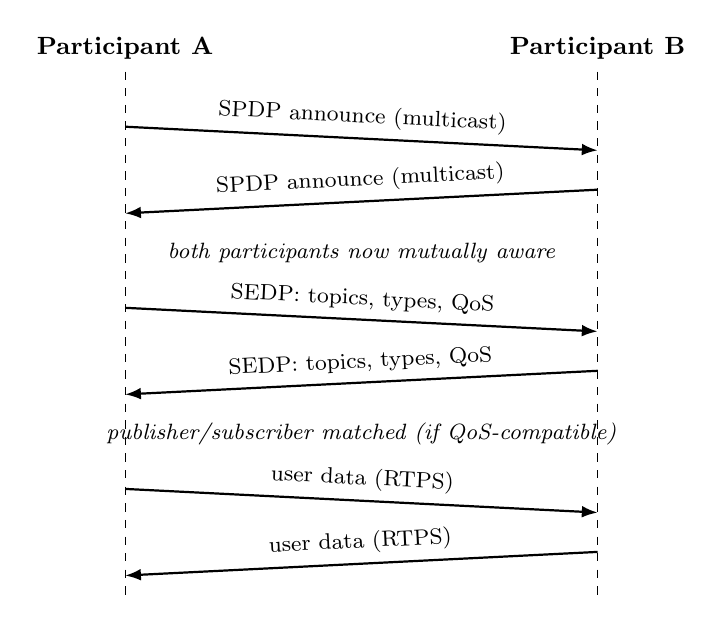
\begin{tikzpicture}[
      participant/.style={font=\small\bfseries},
      msg/.style={-{Latex[length=2mm]}, thick},
      every node/.style={font=\footnotesize}
    ]
    \node[participant] (A) at (0,0) {Participant A};
    \node[participant] (B) at (6,0) {Participant B};
    \draw[dashed] (0,-0.3) -- (0,-7);
    \draw[dashed] (6,-0.3) -- (6,-7);

    \draw[msg] (0,-1) -- (6,-1.3) node[midway,above,sloped] {SPDP announce (multicast)};
    \draw[msg] (6,-1.8) -- (0,-2.1) node[midway,above,sloped] {SPDP announce (multicast)};
    \node[align=center] at (3,-2.6) {\itshape both participants now mutually aware};

    \draw[msg] (0,-3.3) -- (6,-3.6) node[midway,above,sloped] {SEDP: topics, types, QoS};
    \draw[msg] (6,-4.1) -- (0,-4.4) node[midway,above,sloped] {SEDP: topics, types, QoS};
    \node[align=center] at (3,-4.9) {\itshape publisher/subscriber matched (if QoS-compatible)};

    \draw[msg] (0,-5.6) -- (6,-5.9) node[midway,above,sloped] {user data (RTPS)};
    \draw[msg] (6,-6.4) -- (0,-6.7) node[midway,above,sloped] {user data (RTPS)};
  \end{tikzpicture}
  \caption[DDS discovery: SPDP and SEDP stages]{DDS discovery, in two stages, before any user data is exchanged: SPDP lets participants become mutually aware with no central broker; SEDP then matches individual publishers to subscribers by topic, type and QoS. Both stages are themselves messages on the versioned RTPS wire protocol. If either side fails to parse the other's SPDP/SEDP messages (e.g.\ due to a protocol-version mismatch), the process stops here with no error raised on either side, exactly the ``silent failure'' Section~\ref{sec:rmw-incompatibility} diagnosed on hardware.}
  \label{fig:dds-discovery}
\end{figure}

QoS policies add a second, independent way for two otherwise
discoverable endpoints to fail to exchange data -- this time by
\emph{design}, not by defect. DDS defines an explicit compatibility
rule per policy, evaluated during SEDP matching: a subscriber may
request a QoS \emph{no stronger} than what a publisher offers
(Table~\ref{tab:qos-compatibility}) \cite{omg2015dds}. A subscriber
requesting a stronger policy than the publisher offers on that
dimension is a declared incompatibility. DDS silently does not
match that pair. Again, an application-level developer would learn
nothing about this without independently comparing the two sides'
QoS settings.

\begin{table}[htbp]
  \centering
  \caption{QoS compatibility rule for the two policies relevant to this thesis (strongest requestable value shown first).}
  \label{tab:qos-compatibility}
  \begin{tabular}{@{}lll@{}}
    \toprule
    Policy & Publisher offers & Subscriber may request \\
    \midrule
    Reliability & \texttt{RELIABLE} & \texttt{RELIABLE} or \texttt{BEST\_EFFORT} \\
    Reliability & \texttt{BEST\_EFFORT} & \texttt{BEST\_EFFORT} only \\
    Durability & \texttt{TRANSIENT\_LOCAL} & \texttt{TRANSIENT\_LOCAL} or \texttt{VOLATILE} \\
    Durability & \texttt{VOLATILE} & \texttt{VOLATILE} only \\
    \bottomrule
  \end{tabular}
\end{table}

By this rule, a \texttt{VOLATILE} subscriber against a
\texttt{TRANSIENT\_LOCAL} publisher is formally compatible. This is
exactly the configuration Section~\ref{sec:monitor-goal-timing}
found, on QCar, delivering zero messages in practice
despite being spec-compliant.

Section~\ref{sec:monitor-goal-timing} discusses the likely practical
reason. Durability governs whether \emph{historical}, already-published
samples are replayed to a late-joining subscriber, not merely
whether future ones are delivered. A \texttt{VOLATILE} subscriber
that joins after a transient-local publisher's relevant samples were
already sent may receive none of the backlog and then simply waits
for a next sample -- one that, for a low-frequency topic like action
status, may not arrive for a long time.

The point for this chapter is the general one: formal QoS
compatibility, as defined by the DDS specification, is a necessary
but not sufficient condition for an application to actually observe
the message flow it expects.

\subsection{The Action Interface and Goal Lifecycle}
\label{sec:action-lifecycle}

Nav2's \texttt{navigate\_to\_pose} interface, used throughout
Chapter~\ref{ch:nav-integration}, is a ROS~2 \emph{action}
\cite{macenski2022ros2}. Rather than being a distinct transport, an
action is built on top of topics and services: it pairs a
goal-request service call with two topics the server publishes on. A
feedback topic carries periodic progress updates. A status topic
reports each known goal's current state as one of a fixed
enumeration (\texttt{ACCEPTED}, \texttt{EXECUTING},
\texttt{CANCELING}, \texttt{SUCCEEDED}, \texttt{CANCELED},
\texttt{ABORTED}, among others).

The status topic uses \texttt{TRANSIENT\_LOCAL} durability, the same
property discussed above. This lets a subscriber that starts
listening partway through a goal's execution recover its current
state from the retained history, rather than being blind until the
next status change.

Status updates are only published when the server's internal state
machine actually transitions. The status topic's history depth
is finite. This means a fast state machine can advance through more
than one transition between two publishes that an external observer
actually receives. There is no guarantee that every individual state
is observable -- only that the \emph{latest} state at any polling
instant is correct.

Section~\ref{sec:monitor-goal-timing} documents exactly this: a goal
was observed to skip directly from absent to \texttt{EXECUTING} in
one status message, with no separately observable \texttt{ACCEPTED}
update in between. The server's internal state machine does pass
through \texttt{ACCEPTED} on its way to \texttt{EXECUTING} -- the
transition happened, but no status publish was ever emitted while it
was current in isolation. This is a general property of polling a
periodically published state summary, not a special case of this one
topic.

\section{Ackermann Steering Kinematics}
\label{sec:ackermann-kinematics}

The QCar is a rear-wheel-drive vehicle with front-wheel Ackermann
steering \cite{snider2009pathtracking}. The two front wheels pivot
independently about near-vertical steering axes, such that for any
commanded steering angle, both front wheels' instantaneous velocity
vectors are perpendicular to lines drawn through a single common
point on the extended rear axle. This point is the vehicle's
instantaneous centre of rotation. This geometric constraint means the
two front wheels must generally be steered to slightly different
angles, with the inner wheel turning more sharply than the outer, so
that all four wheels roll without slipping through a common turn
centre.

For control and estimation purposes, this thesis follows the
standard simplification to a single-track bicycle model
\cite{snider2009pathtracking}, which replaces the two front wheels with
a single virtual wheel at the centre of the front axle steered at
angle $\delta$ and the two rear wheels with a single virtual wheel
at the centre of the rear axle. With vehicle heading $\theta$,
wheelbase $L$ (the longitudinal distance between the front and rear
axles) and rear-axle speed $v$, the kinematic bicycle model is:

\begin{align}
  \dot{x} &= v \cos\theta \label{eq:bicycle-x}\\
  \dot{y} &= v \sin\theta \label{eq:bicycle-y}\\
  \dot{\theta} &= \frac{v}{L}\tan\delta \label{eq:bicycle-theta}
\end{align}

and the corresponding instantaneous turning radius about the rear
axle is

\begin{equation}
  R = \frac{L}{\tan\delta}. \label{eq:bicycle-radius}
\end{equation}

Equation~\ref{eq:bicycle-theta} is the basis of the onboard bridge's
dead-reckoning odometry described in Chapter~\ref{ch:hardware-bridge},
which genuinely integrates wheel-encoder and commanded-steering
readings forward through this relationship at every control cycle to
estimate pose from scratch. A single-track model is a simplification: it assumes no lateral tyre
slip and treats both front wheels as a single steering angle rather
than the true Ackermann-differentiated pair. Chapter~\ref{ch:calibration}
presents direct evidence of where this simplification's limits were
reached in practice on QCar
(Section~\ref{sec:deadband-discovery}).

\subsection{The True Two-Wheel Ackermann Angle}
\label{sec:true-ackermann}

The single-track model above is a control- and estimation-time
convenience. It is not what the Gazebo drive plugin actually
commands at the level of the two physical front wheels.

Because the two front wheels steer about laterally separated axes, a
single-track model's one steering angle $\delta$ must generally be
converted into two slightly different angles, with the inner wheel
(on the side the vehicle is turning toward) steered more sharply than
the outer. This ensures both front wheels' rolling directions remain
tangent to circles sharing the same centre on the extended rear axle.
This is the condition for rolling without slipping introduced in
Section~\ref{sec:ackermann-kinematics}'s opening paragraph. With
track width $T$ (the lateral distance between
the two front steering axes) and wheelbase $L$, the exact left- and
right-wheel steering angles corresponding to a single-track angle
$\delta$ are:

\begin{align}
  \delta_{\text{left}} &= \operatorname{atan2}\!\left(\tan\delta,\ 1 - \dfrac{T}{2L}\tan\delta\right) \label{eq:ackermann-left}\\
  \delta_{\text{right}} &= \operatorname{atan2}\!\left(\tan\delta,\ 1 + \dfrac{T}{2L}\tan\delta\right) \label{eq:ackermann-right}
\end{align}

(signed so that a positive $\delta$, a left turn, gives
$\delta_{\text{left}} > \delta_{\text{right}}$ -- the inside wheel of
the turn steers further). This is precisely the pair of relationships
the \texttt{gazebo\_ros\_ackermann\_drive} plugin evaluates every
simulation step from a single commanded angular velocity.
Chapter~\ref{ch:sim-stack} also refers to this same formula when
describing the plugin auto-computing Ackermann geometry from URDF
joint positions:
$T$ and $L$ in Equations~\ref{eq:ackermann-left}--\ref{eq:ackermann-right}
are measured directly from the URDF's own front-hub joint origins at
spawn time, never stated as separate configuration values.

As $T \to 0$ (a vanishingly narrow front track), both angles converge
to the single-track $\delta$. This confirms
Equations~\ref{eq:ackermann-left}--\ref{eq:ackermann-right} correctly
generalise, rather than contradict, the simpler model of
Equations~\ref{eq:bicycle-x}--\ref{eq:bicycle-theta}.

\begin{table}[htbp]
  \centering
  \caption{QCar Ackermann geometry parameters used throughout this thesis.}
  \label{tab:qcar-geometry}
  \begin{tabular}{@{}lll@{}}
    \toprule
    Parameter & Value & Source \\
    \midrule
    Wheelbase $L$ & \SI{0.25725}{\meter} & URDF joint geometry (measured) \\
    Front track width & \SI{0.1118}{\meter} & URDF joint geometry (measured) \\
    Rear track width & \SI{0.1122}{\meter} & URDF joint geometry (measured) \\
    Wheel radius & \SI{0.033}{\meter} & Wheel mesh bounding box (measured) \\
    Max.\ steering angle $\delta_{max}$ & \SI{0.5236}{\radian} (\ang{30}) & Vehicle/plugin limit \\
    Min.\ turning radius (from Eq.~\ref{eq:bicycle-radius}) & \SI{0.446}{\meter} & Derived \\
    \bottomrule
  \end{tabular}
\end{table}

\begin{figure}[htbp]
  \centering
  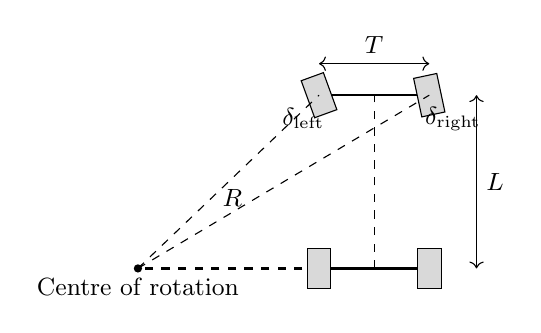
\begin{tikzpicture}[scale=1.0, every node/.style={font=\small}]
    \coordinate (RL) at (-0.7,0);
    \coordinate (RR) at (0.7,0);
    \coordinate (FL) at (-0.7,2.2);
    \coordinate (FR) at (0.7,2.2);
    \coordinate (C) at (-3.0,0);

    \draw[thick] (RL) -- (RR);
    \draw[thick] (FL) -- (FR);
    \draw[thick,dashed] (RL) -- (C);
    \draw[dashed] (0,0) -- (0,2.2);

    \draw[fill=gray!30] (RL) ++(-0.15,-0.25) rectangle ++(0.3,0.5);
    \draw[fill=gray!30] (RR) ++(-0.15,-0.25) rectangle ++(0.3,0.5);

    \begin{scope}[rotate around={20:(FL)}]
      \draw[fill=gray!30] (FL) ++(-0.15,-0.25) rectangle ++(0.3,0.5);
    \end{scope}
    \begin{scope}[rotate around={12:(FR)}]
      \draw[fill=gray!30] (FR) ++(-0.15,-0.25) rectangle ++(0.3,0.5);
    \end{scope}

    \fill (C) circle (1.5pt);
    \node[below] at (C) {Centre of rotation};

    \draw[dashed] (C) -- (FL);
    \draw[dashed] (C) -- (FR);

    \draw[<->] (1.3,0) -- (1.3,2.2) node[midway,right] {$L$};
    \draw[<->] (-0.7,2.6) -- (0.7,2.6) node[midway,above] {$T$};

    \node at (-0.9,1.9) {$\delta_{\text{left}}$};
    \node at (1.0,1.9) {$\delta_{\text{right}}$};
    \node at (-1.8,0.9) {$R$};
  \end{tikzpicture}
  \caption[Ackermann steering geometry]{Ackermann steering geometry (top-down view, not to scale): the two front wheels are steered to different angles $\delta_{\text{left}} > \delta_{\text{right}}$ (left turn shown) so that lines through both front wheels' rolling directions and the rear axle all intersect at a single centre of rotation. Wheelbase $L$ and track width $T$ are the parameters of Equations~\ref{eq:ackermann-left}--\ref{eq:ackermann-right}.}
  \label{fig:ackermann-geometry}
\end{figure}

\section{Simulation with Gazebo}
\label{sec:gazebo}

Gazebo is a physics-based 3D robot simulator, originally built around
a rigid-body dynamics engine, a small set of sensor models (odometry,
ray-proximity/laser range-finding and camera) and a modular
client/interface layer for injecting control logic into simulated
models without coupling that logic to the physics engine itself
\cite{koenig2004gazebo}.

Two later generations of Gazebo are relevant to this project's
history. Both are architecturally distinct from each other and both
extend the original model with a formal SDF-based plugin system and a
substantially wider sensor suite, including LiDAR and IMU sensor
models. Only the LiDAR model is actually used in this project's
simulation stack (see the IMU note in
Section~\ref{sec:qcar-platform}). \emph{Gazebo Classic} (versions up
to 11) integrates with ROS~2 through the separate
\texttt{gazebo\_ros} / \texttt{gazebo\_plugins} packages, while the
newer \emph{Gazebo Sim} (formerly Ignition Gazebo) integrates through
\texttt{ros\_gz\_sim} / \texttt{ros\_gz\_bridge}.

The two are not drop-in replacements for each other. Plugin
filenames, topic remapping mechanisms and world-file (SDF) syntax
for built-in physics/sensor systems all differ between them. A
package written against one will not load under the other without a
systematic conversion.

This project uses Gazebo Classic~11 with the \texttt{gazebo\_ros}
family of plugins, matching the ROS~2 Humble / Ubuntu 22.04 host
environment, in which Gazebo Sim's binaries are not available at
all.

The robot itself is described in the Unified Robot Description
Format (URDF), an XML dialect specifying the vehicle's kinematic
tree (links and joints), visual meshes and collision geometry. A
\texttt{<gazebo>} block within the URDF attaches simulation-only
elements: sensor definitions and the drive plugin
(\texttt{libgazebo\_ros\_ackermann\_drive.so}) that subscribes to
\texttt{/cmd\_vel} and converts commanded linear/angular velocity
into per-wheel drive and steering-hub joint efforts. It uses the
Ackermann geometry of Section~\ref{sec:ackermann-kinematics} for
this, auto-computed from the URDF's own joint and collision geometry
at spawn time rather than restated in a separate configuration file.

A recurring practical property of this plugin, directly relevant to
Chapter~\ref{ch:sim-stack}, is that its wheel-radius auto-detection
only supports primitive collision shapes (cylinders, spheres). A
mesh-shaped wheel collision silently yields a wheel radius of zero,
which propagates as a division-by-zero into the plugin's velocity
PID controller.

Simulated friction is likewise not automatic: both the wheel links
and the ground plane must be assigned explicit Coulomb friction
coefficients (SDF's \texttt{mu1}/\texttt{mu2}) or the simulated
vehicle exhibits perfect wheel slip with no resulting translation,
regardless of commanded wheel speed. Neither failure mode raises an
error. Both look, from the outside, like ``the robot is not
moving.'' Both are addressed in detail in
Section~\ref{sec:not-moving-bug}.

\subsection{The Plugin's PID Control Loop and the Physics Step}
\label{sec:gazebo-pid-loop}

The drive plugin does not run on its own timer. It registers a
callback on Gazebo's \texttt{WorldUpdateBegin} event, which fires
once per physics step of the rigid-body solver -- by default
\SI{1}{\milli\second} of simulated time per step, i.e.\
\SI{1000}{\hertz}, independent of and generally much faster than any
ROS~2 topic rate in the system.

On every physics step, regardless of whether a new
\texttt{/cmd\_vel} message has arrived, the callback re-reads the
rear wheel's current angular velocity from the physics engine. It
compares that reading against the most recently \emph{commanded}
linear velocity, converted to an equivalent target angular velocity
($\text{target\_linear} / \text{wheel\_radius}$) and passes the
resulting error through a discrete PID controller. The controller's
output is applied directly as a joint \emph{force} (torque), not a
velocity: this is a torque-controlled velocity-tracking loop, not a
kinematic teleport of the wheel to a commanded speed. The controller
update takes the classical form \cite{astrom2008feedback}

\begin{equation}
  u(t) = K_p\, e(t) + K_i \int_0^t e(\tau)\, \mathrm{d}\tau + K_d \frac{\mathrm{d}e(t)}{\mathrm{d}t},
  \qquad e(t) = \text{measured}(t) - \text{target}(t),
  \label{eq:pid}
\end{equation}

evaluated once per physics step, with the integral and derivative
terms accumulated or estimated over the actual, possibly
non-uniform, time elapsed since the previous step. The integral term
can optionally be clamped to a configured $[i_{\min}, i_{\max}]$
range, to prevent unbounded windup while the system is far from its
target.

Three independent instances of this controller run inside the
plugin: one for the rear-axle drive velocity and one each for the
left and right steering hubs, tracking the two Ackermann angles of
Equations~\ref{eq:ackermann-left}--\ref{eq:ackermann-right}
independently rather than as a single shared steering command. All
three sets of gains ($K_p$, $K_i$, $K_d$) are declared per-vehicle in
the URDF's \texttt{<gazebo>} plugin block. Section~\ref{sec:not-moving-bug}
documents in detail what happens when these gains are tuned for one
physical configuration (e.g.\ frictionless wheels) and then reused
unchanged after that configuration changes.

Equation~\ref{eq:pid} also explains precisely why the wheel-radius
defect above is destructive rather than merely inaccurate. With
$\text{wheel\_radius} = 0$, the target angular velocity
$\text{target\_linear}/\text{wheel\_radius}$ is not merely wrong --
it is unbounded for any nonzero commanded linear velocity. That
makes $e(t)$ itself unbounded, driving the PID controller to its
output saturation limit (or to a floating-point infinity/NaN)
regardless of how the three gains are tuned. No amount of gain
retuning can compensate for an error signal that is not a finite
number in the first place, which is why this class of bug survives
naive ``just tune the PID harder'' troubleshooting.

\begin{figure}[htbp]
  \centering
  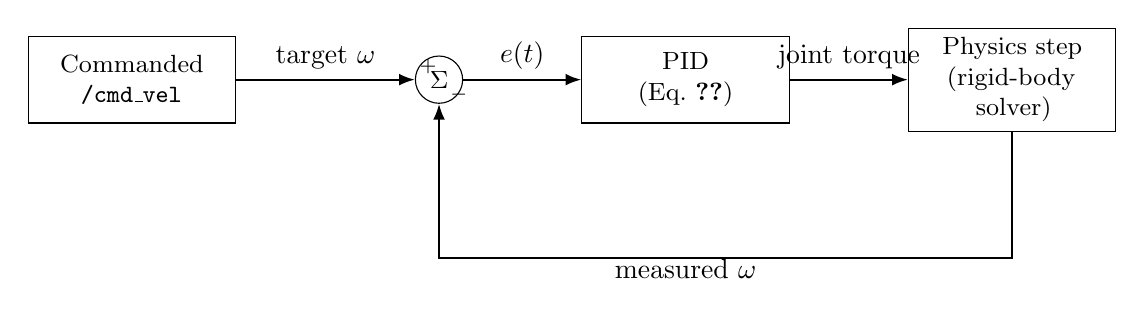
\begin{tikzpicture}[
      block/.style={draw, rectangle, minimum height=1.1cm, text width=2.4cm, align=center, font=\small},
      sum/.style={draw, circle, minimum size=0.6cm, font=\small, inner sep=0pt},
      arr/.style={-{Latex[length=2mm]}, thick},
      node distance=1.5cm
    ]
    \node[block] (cmd) at (0,0) {Commanded\\\texttt{/cmd\_vel}};
    \node[sum] (sum) at (3.9,0) {$\Sigma$};
    \node[block] (pid) [right=of sum] {PID\\(Eq.~\ref{eq:pid})};
    \node[block] (plant) [right=of pid] {Physics step\\(rigid-body solver)};

    \draw[arr] (cmd) -- (sum) node[midway,above] {target $\omega$};
    \draw[arr] (sum) -- (pid) node[midway,above] {$e(t)$};
    \draw[arr] (pid) -- (plant) node[midway,above] {joint torque};

    \draw[arr] (plant.south) -- ++(0,-1.6) -| (sum.south);
    \node[below] at ($(pid.south)+(0,-1.6)$) {measured $\omega$};

    \node at ($(sum.north west)+(0.08,-0.05)$) {\scriptsize $+$};
    \node at ($(sum.south)+(0.25,0.12)$) {\scriptsize $-$};
  \end{tikzpicture}
  \caption[The drive plugin's per-wheel PID control loop]{The drive plugin's per-wheel torque control loop, re-evaluated every Gazebo physics step (\SI{1}{\kilo\hertz}): a commanded velocity is converted to a target angular velocity, compared against the physics engine's own measured wheel angular velocity to form an error $e(t)$ and passed through Equation~\ref{eq:pid}'s PID controller, whose output is applied directly as a joint torque. Three independent instances of this loop run per vehicle (drive, left steering, right steering).}
  \label{fig:pid-loop}
\end{figure}

\subsection{Contact Friction via the Coulomb Model and Friction Cone}
\label{sec:friction-theory}

Gazebo Classic's default physics engine, the Open Dynamics Engine
(ODE), models contact friction at each collision point using a
Coulomb friction approximation \cite{oderelease}: the maximum
tangential (sliding) force a contact can sustain before slipping is
proportional to the normal (compressive) force pressing the two
surfaces together, with the constant of proportionality being the
friction coefficient $\mu$. ODE further allows this coefficient to be
specified separately along two orthogonal directions in the contact
plane (\texttt{mu1}/\texttt{mu2} in the URDF/SDF). A tyre could in
principle grip differently along its rolling direction than sideways
across it, though this project sets both equal -- isotropic
friction. ODE itself approximates the true (circular)
Coulomb friction cone in one of two ways: a default ``constant-force-limit''
mode, where $\mu$ is treated as an absolute force limit independent
of the actual normal force or a more physically accurate ``friction
pyramid'' approximation, enabled via the \texttt{dContactApprox1}
contact flag \cite{oderelease}. This project does not override
either setting. The URDF's \texttt{<gazebo>} friction blocks
(Listing~\ref{lst:wheel-collision-friction}) set only
\texttt{mu1}/\texttt{mu2}, leaving Gazebo Classic's own default
friction-approximation mode in effect. The isotropic $\mu=1.0$ value
chosen is what actually mattered for fixing the zero-friction bug
below, not which of the two approximation modes was active.

Critically, \textbf{ODE applies no friction at all to a contact whose
$\mu_1$/$\mu_2$ default to zero}. There is no implicit ``reasonable
default'' friction coefficient assumed for an unconfigured surface,
unlike, say, a default coefficient of restitution.

This is precisely why Section~\ref{sec:not-moving-bug}'s bug~2 (zero
wheel friction) produces literal, total 100\% slip rather than
merely reduced traction. With $\mu = 0$, the Coulomb limit on
tangential force is zero regardless of how hard the wheel presses
into the ground. No sliding friction force can develop at all, no
matter how fast the wheel itself spins, so no forward thrust on the
chassis can develop either.

\section{Simultaneous Localization and Mapping with Cartographer}
\label{sec:cartographer}

Simultaneous Localization and Mapping (SLAM) is the problem of
building a map of an unknown environment while concurrently
estimating the robot's pose within that same map, using only the
robot's own sensor stream and (optionally) odometry
\cite{cadena2016slam}. This thesis uses
Google's Cartographer \cite{hess2016cartographer}, a real-time 2D/3D
LiDAR SLAM system that performs local scan matching to build
submaps and a global pose-graph optimisation to detect and correct
loop closures. It is exposed to ROS~2 via the
\texttt{cartographer\_ros} package.

Cartographer can either fuse external odometry into its
scan-matching prediction or perform scan-matching-only pose
estimation (\texttt{use\_odometry: false}). In the latter case, it
also provides the full \texttt{map} $\rightarrow$ \texttt{odom}
$\rightarrow$ \texttt{base} transform (TF) chain itself
(\texttt{provide\_odom\_frame: true}), rather than expecting an
external odometry source to supply the \texttt{odom} $\rightarrow$
\texttt{base} portion.

This configuration choice was made for this project's mapping
pipeline and is detailed in Chapter~\ref{ch:hardware-bridge}. It
turned out to remove an entire class of TF-ownership conflict
between Cartographer and the vehicle's own drive-plugin odometry
that would otherwise arise, since ROS~2's TF system permits only one
broadcaster per transform edge at a time without producing
ambiguous, jittering results.

\section{The Nav2 Navigation Stack}
\label{sec:nav2}

Nav2 is the ROS~2 successor to the ROS~1 navigation stack, providing
a modular, plugin-based pipeline for autonomous point-to-point
navigation against a known (or concurrently built) map
\cite{macenski2020nav2}. Its major components, all used in this
thesis, are:

\begin{description}
  \item[Costmaps] Layered 2D occupancy grids
    \cite{elfes1989occupancy} (static map layer, obstacle/LiDAR
    layer, inflation layer) that represent both the known static
    environment and dynamically observed obstacles as traversability
    cost, separately for global path planning and local trajectory
    control.
  \item[AMCL (Adaptive Monte Carlo Localization)] A particle-filter
    localisation algorithm that maintains a probability distribution
    over the robot's pose as a weighted set of discrete pose
    hypotheses (particles), resampled according to how well each
    particle's predicted LiDAR scan matches the actual scan against
    the static map. This follows the Monte Carlo localisation method
    \cite{dellaert1999mcl}, presented here in the probabilistic
    framework used throughout this section \cite{thrun2000probrob}.
    AMCL's motion-model noise parameters (commonly denoted
    $\alpha_1$--$\alpha_5$) control how much particle spread is
    injected per unit of commanded motion. Chapter~\ref{ch:nav-integration}
    documents a real localisation failure mode and its correction,
    tied directly to these parameters.
  \item[Global planning] Nav2's \texttt{SmacPlannerHybrid} plugin,
    used in this project, plans a kinematically feasible path using a
    hybrid-state A* search with a Reeds-Shepp motion primitive set
    \cite{dolgov2008hybridastar}. A Reeds-Shepp curve is the shortest
    path between two poses for a car-like vehicle with a bounded
    turning radius that can move both forward and backward, built from
    straight-line segments and constant-curvature arcs -- unlike a
    Dubins curve, which assumes forward motion only and so cannot
    represent a reversing manoeuvre at all. This respects the vehicle's
    minimum turning radius (Table~\ref{tab:qcar-geometry}) and allows a
    reversing segment where one is genuinely required, rather than
    planning paths the physical vehicle cannot actually follow.
  \item[Local trajectory control: MPPI] Model Predictive Path
    Integral control \cite{williams2015mppi} is a sampling-based
    model-predictive control method. At each control cycle, a large
    number ($\mathcal{O}(1000)$) of candidate control sequences are
    simulated forward through a vehicle model over a fixed horizon.
    Each rollout is scored by a weighted sum of cost terms --
    \emph{critics} in Nav2's terminology, covering path alignment,
    path following, goal distance, obstacle cost and others. The
    executed control is then an importance-weighted average across
    all sampled rollouts, not the single lowest-cost trajectory.
    This avoids the need for a convex, analytically differentiable
    cost function or vehicle model, at the cost of requiring many
    parallel forward simulations per control cycle. Nav2's MPPI
    controller plugin supports custom critic plugins loaded
    alongside the stock set. Section~\ref{sec:mppi-critic} describes
    a custom critic developed as part of this project's navigation
    stack.
  \item[Behavior Trees] Nav2 orchestrates recovery behaviours (costmap
    clearing, spinning in place, waiting, backing up) and overall
    navigation logic via an externally configurable behaviour tree
    (BT) \cite{colledanchise2018bt}, rather than hard-coded state
    machine logic. This allows per-robot customisation of, for
    instance, which recovery actions are physically valid for a given
    platform. It is directly relevant to Section~\ref{sec:bt-fix},
    where the stock recovery tree's default in-place \texttt{Spin}
    action is shown to be physically unachievable for an
    Ackermann-steered vehicle.
\end{description}

\subsection{MPPI's Sampling, Scoring and Softmax Update in Detail}
\label{sec:mppi-math}

MPPI's central idea is to replace the search for a single optimal
control sequence with a weighted average over many randomly
perturbed candidates, where the weighting itself is derived from an
information-theoretic optimality argument rather than chosen
heuristically \cite{williams2015mppi}. Concretely,
given a current nominal control sequence
$\mathbf{u} = (u_0, \ldots, u_{T-1})$ over a horizon of $T$ steps,
the controller draws $K$ independent perturbed sequences

\begin{equation}
  u_t^{(k)} = u_t + \varepsilon_t^{(k)}, \qquad \varepsilon_t^{(k)} \sim \mathcal{N}(0, \Sigma), \quad k = 1, \ldots, K,
  \label{eq:mppi-sample}
\end{equation}

rolls each one forward through the vehicle model (the Ackermann
bicycle model of Section~\ref{sec:ackermann-kinematics}, in this
project's configuration) to obtain a full predicted trajectory
$\tau^{(k)}$ and evaluates a total cost $S(\tau^{(k)})$ for each. In
Nav2's implementation, this total cost is exactly the running sum
that every enabled critic plugin adds into via a single shared
per-trajectory accumulator, including the custom
\texttt{EarlyCommitCritic} of Section~\ref{sec:mppi-critic}.
Section~\ref{sec:mppi-critic}'s critic therefore contributes one
additive term among several to $S(\tau^{(k)})$, not a separate
decision stage. Trajectories are then combined into an updated
control sequence via an importance-sampling weighted average:

\begin{equation}
  w^{(k)} = \frac{\exp\!\left(-\frac{1}{\lambda}\left(S(\tau^{(k)}) - \rho\right)\right)}
                 {\sum_{j=1}^{K} \exp\!\left(-\frac{1}{\lambda}\left(S(\tau^{(j)}) - \rho\right)\right)},
  \qquad
  u_t^{\text{new}} = \sum_{k=1}^{K} w^{(k)}\, u_t^{(k)},
  \label{eq:mppi-weight}
\end{equation}

where $\rho = \min_k S(\tau^{(k)})$ is subtracted purely for
numerical stability, so the largest exponent evaluated is always
zero. $\lambda > 0$ is a temperature parameter controlling how
sharply the weighting favours the very lowest-cost rollouts: as
$\lambda \to 0$, Equation~\ref{eq:mppi-weight} approaches a hard
arg-min over the sampled trajectories, while larger $\lambda$
approaches a uniform average across all of them, largely ignoring
cost.

Only the first control $u_0^{\text{new}}$ of the updated sequence is
actually sent to the vehicle each control cycle. The whole horizon
is then shifted by one step and the process repeats. This is the
standard receding-horizon pattern shared with other model-predictive
control methods, but arrived at here via random sampling and a
softmax-like weighted average, rather than a gradient- or search-based
optimisation over a differentiable cost surface.

This is precisely why MPPI tolerates the sharply non-smooth,
hand-crafted critic terms used throughout Nav2, including a critic
like \texttt{EarlyCommitCritic} that is not differentiable in any
convenient closed form, without requiring them to be reformulated as
a smooth, gradient-friendly cost function first.

\begin{figure}[htbp]
  \centering
  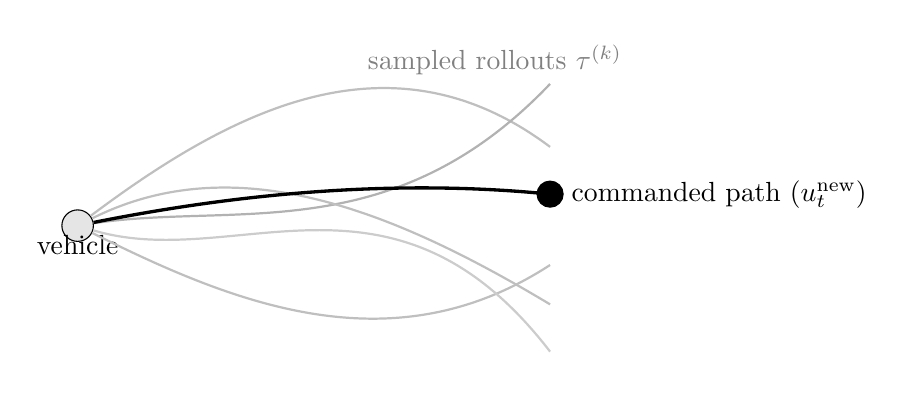
\begin{tikzpicture}[scale=1.0]
    \node[draw,circle,fill=gray!20,minimum size=0.4cm] (start) at (0,0) {};
    \node[below] at (start) {vehicle};

    \draw[gray!50, thick] (start) .. controls (2,1.5) and (4,2.5) .. (6,1.0);
    \draw[gray!50, thick] (start) .. controls (2,-1.0) and (4,-1.8) .. (6,-0.5);
    \draw[gray!60, thick] (start) .. controls (2,0.3) and (4,-0.3) .. (6,1.8);
    \draw[gray!40, thick] (start) .. controls (2,-0.6) and (4,1.0) .. (6,-1.6);
    \draw[gray!50, thick] (start) .. controls (2,1.0) and (4,0.2) .. (6,-1.0);

    \draw[very thick] (start) .. controls (2,0.4) and (4,0.6) .. (6,0.4);
    \node[draw,circle,fill=black,minimum size=0.15cm] at (6,0.4) {};
    \node[right] at (6.15,0.4) {commanded path ($u_t^{\text{new}}$)};

    \node[gray] at (5.3,2.1) {sampled rollouts $\tau^{(k)}$};
  \end{tikzpicture}
  \caption[MPPI's sampling-based control update]{MPPI's sampling-based control update: $K$ randomly perturbed control sequences are each rolled forward through the vehicle model into a candidate trajectory $\tau^{(k)}$ (grey), each scored by the total critic cost $S(\tau^{(k)})$; Equation~\ref{eq:mppi-weight}'s softmax weighting then combines all $K$ trajectories into one commanded control sequence (black). Lower-cost rollouts contribute more weight, but every sampled trajectory contributes something, unlike a hard arg-min over a discrete set of candidates.}
  \label{fig:mppi-concept}
\end{figure}

\subsection{AMCL's Particle Filter and Recovery Mechanism in Detail}
\label{sec:amcl-math}

AMCL maintains its belief about the robot's pose as a set of $N$
weighted particles $\{(x^{(i)}, w^{(i)})\}_{i=1}^{N}$, each a
concrete pose hypothesis, updated on every new odometry/LiDAR pair
through the standard Monte Carlo localisation prediction-update-resample
cycle \cite{thrun2000probrob}:

\begin{enumerate}
  \item \textbf{Prediction (motion model).} Each particle is
    propagated forward using the commanded/odometric motion since the
    last update, corrupted by noise whose magnitude is controlled by
    the $\alpha_1$--$\alpha_4$ parameters mentioned in the component
    list above (roughly: $\alpha_1$/$\alpha_2$ scale rotational noise
    from the odometry's rotational and translational components
    respectively, $\alpha_3$/$\alpha_4$ scale translational noise the
    same way). Larger values inject more particle spread per unit of
    commanded motion, modelling greater distrust in odometry.
  \item \textbf{Update (measurement model).} Each particle's weight
    is set proportional to the likelihood of the actual LiDAR scan
    given that particle's hypothesised pose and the static map,
    typically via a likelihood-field model that scores each scan
    endpoint by its proximity to the nearest mapped obstacle from that
    hypothesised pose.
  \item \textbf{Resampling.} A new particle set is drawn, with
    replacement, with probability proportional to weight. Particles
    consistent with the actual scan multiply, while inconsistent ones
    are discarded. The particle cloud then statistically converges
    toward the true pose over repeated cycles. AMCL's ``adaptive'' element
    (KLD-sampling) additionally varies $N$ itself between update
    cycles, using fewer particles once the distribution is already
    tightly converged and more while it remains spread out.
\end{enumerate}

\begin{figure}[htbp]
  \centering
  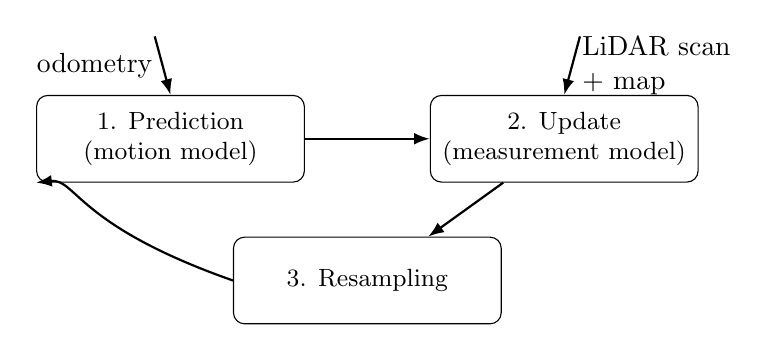
\begin{tikzpicture}[
      block/.style={draw, rectangle, rounded corners, minimum height=1.1cm, minimum width=3.4cm, align=center, font=\small},
      arr/.style={-{Latex[length=2mm]}, thick}
    ]
    \node[block] (predict) at (0,0) {1. Prediction\\(motion model)};
    \node[block] (update) at (5,0) {2. Update\\(measurement model)};
    \node[block] (resample) at (2.5,-1.8) {3. Resampling};

    \draw[arr] (predict) -- (update);
    \draw[arr] (update) -- (resample);
    \draw[arr] (resample.west) .. controls (-1.2,-1.1) and (-1.2,-0.5) .. (predict.south west);

    \draw[arr] (-0.2,1.3) -- (predict.north) node[midway,left,align=right] {odometry};
    \draw[arr] (5.2,1.3) -- (update.north) node[midway,right,align=left] {LiDAR scan\\+ map};
  \end{tikzpicture}
  \caption{The AMCL particle filter's prediction-update-resampling cycle, repeated on every new odometry/LiDAR pair (Section~\ref{sec:amcl-math}).}
  \label{fig:amcl-cycle}
\end{figure}

The parameters directly responsible for the freeze failure mode
documented in Section~\ref{sec:ruled-out} are a separate pair from
the four motion-model $\alpha$s above.
\texttt{recovery\_alpha\_slow}/\texttt{recovery\_alpha\_fast} govern
an \emph{augmented} MCL recovery mechanism: injecting randomly
sampled particles when recent localisation quality drops. This
general concept was evaluated directly against the alternative of
plain MCL, for exactly this kidnapped-robot/recovery scenario, in
\cite{thrun2001robustmcl}.

AMCL's specific implementation of the concept, read directly from
its own parameter documentation and used as configured throughout
this thesis, tracks two exponential moving averages of the particle
set's average weight: a slow long-run average $\bar{w}_{\text{slow}}$
and a fast short-run average $\bar{w}_{\text{fast}}$. Both are
updated after every measurement step, as

\begin{equation}
  \bar{w}_{\text{slow}} \mathrel{+}= \alpha_{\text{slow}}\left(\bar{w} - \bar{w}_{\text{slow}}\right), \qquad
  \bar{w}_{\text{fast}} \mathrel{+}= \alpha_{\text{fast}}\left(\bar{w} - \bar{w}_{\text{fast}}\right),
  \label{eq:amcl-recovery}
\end{equation}

where $\bar{w}$ is the current cycle's average particle weight.

During resampling, instead of drawing every new particle from the
existing weighted set, each new particle is drawn \emph{uniformly at
random from the entire map} with probability $\max\!\left(0,\ 1 -
\bar{w}_{\text{fast}}/\bar{w}_{\text{slow}}\right)$. Intuitively: if
recent particle quality ($\bar{w}_{\text{fast}}$) has dropped
noticeably below the longer-run baseline ($\bar{w}_{\text{slow}}$),
the filter injects fresh, unbiased hypotheses to help it recover
from a bad convergence or a ``kidnapped robot'' scenario, rather than
continuing to resample only from a particle set that may have
already converged to the wrong pose.

This project's simulation-tuned configuration originally inherited
$\alpha_{\text{slow}} = \alpha_{\text{fast}} = 0.0$. At that setting,
neither running average is ever updated from its initial value, so
the random-injection probability is permanently fixed rather than
responsive to real degradation in particle quality. A clean
simulation rarely needs this recovery path at all, but on real,
non-ideal sensor noise, the particle set can converge overconfidently
to an incorrect pose with no mechanism available to reintroduce
diversity. This is the permanent freeze Section~\ref{sec:ruled-out}
reports and fixes, by raising these two parameters off zero.

\section{The Quanser QCar Platform}
\label{sec:qcar-platform}

The physical platform underlying this thesis is the Quanser QCar:
the original platform, not the newer, distinct QCar~2 that Quanser's
documentation set also covers. It is a 1/10th-scale rear-wheel-drive,
Ackermann-steered research vehicle \cite{quanser2023qcar}.

Its onboard computer is an NVIDIA Jetson TX2 system-on-module,
running Ubuntu 18.04 LTS with 32\,GB eMMC storage and Python~3.6.9.
It ships with both ROS~1 Melodic and ROS~2 Dashing pre-installed
side by side, though neither is auto-sourced in the default shell
environment.

The platform additionally ships with an Intel RealSense D435 RGBD
camera, four 360\textdegree{} CSI cameras and an onboard IMU as
standard hardware. This thesis's navigation pipeline uses none of
these. It relies solely on the 2D LiDAR for mapping, localisation
and obstacle sensing, with pose estimation between LiDAR updates
coming from wheel-encoder-based odometry rather than the IMU.

The IMU is electrically present and exposed by QCar's HAL/PAL
library (\texttt{gyroscope/}\allowbreak\texttt{accelerometer} fields), but
nothing in this project's software stack reads it. Cartographer's
\texttt{use\_imu\_data} is left \texttt{false}. No IMU sensor
plugin is declared in the simulation's URDF either, so only the
LiDAR is discussed further.

\begin{figure}[htbp]
  \centering
  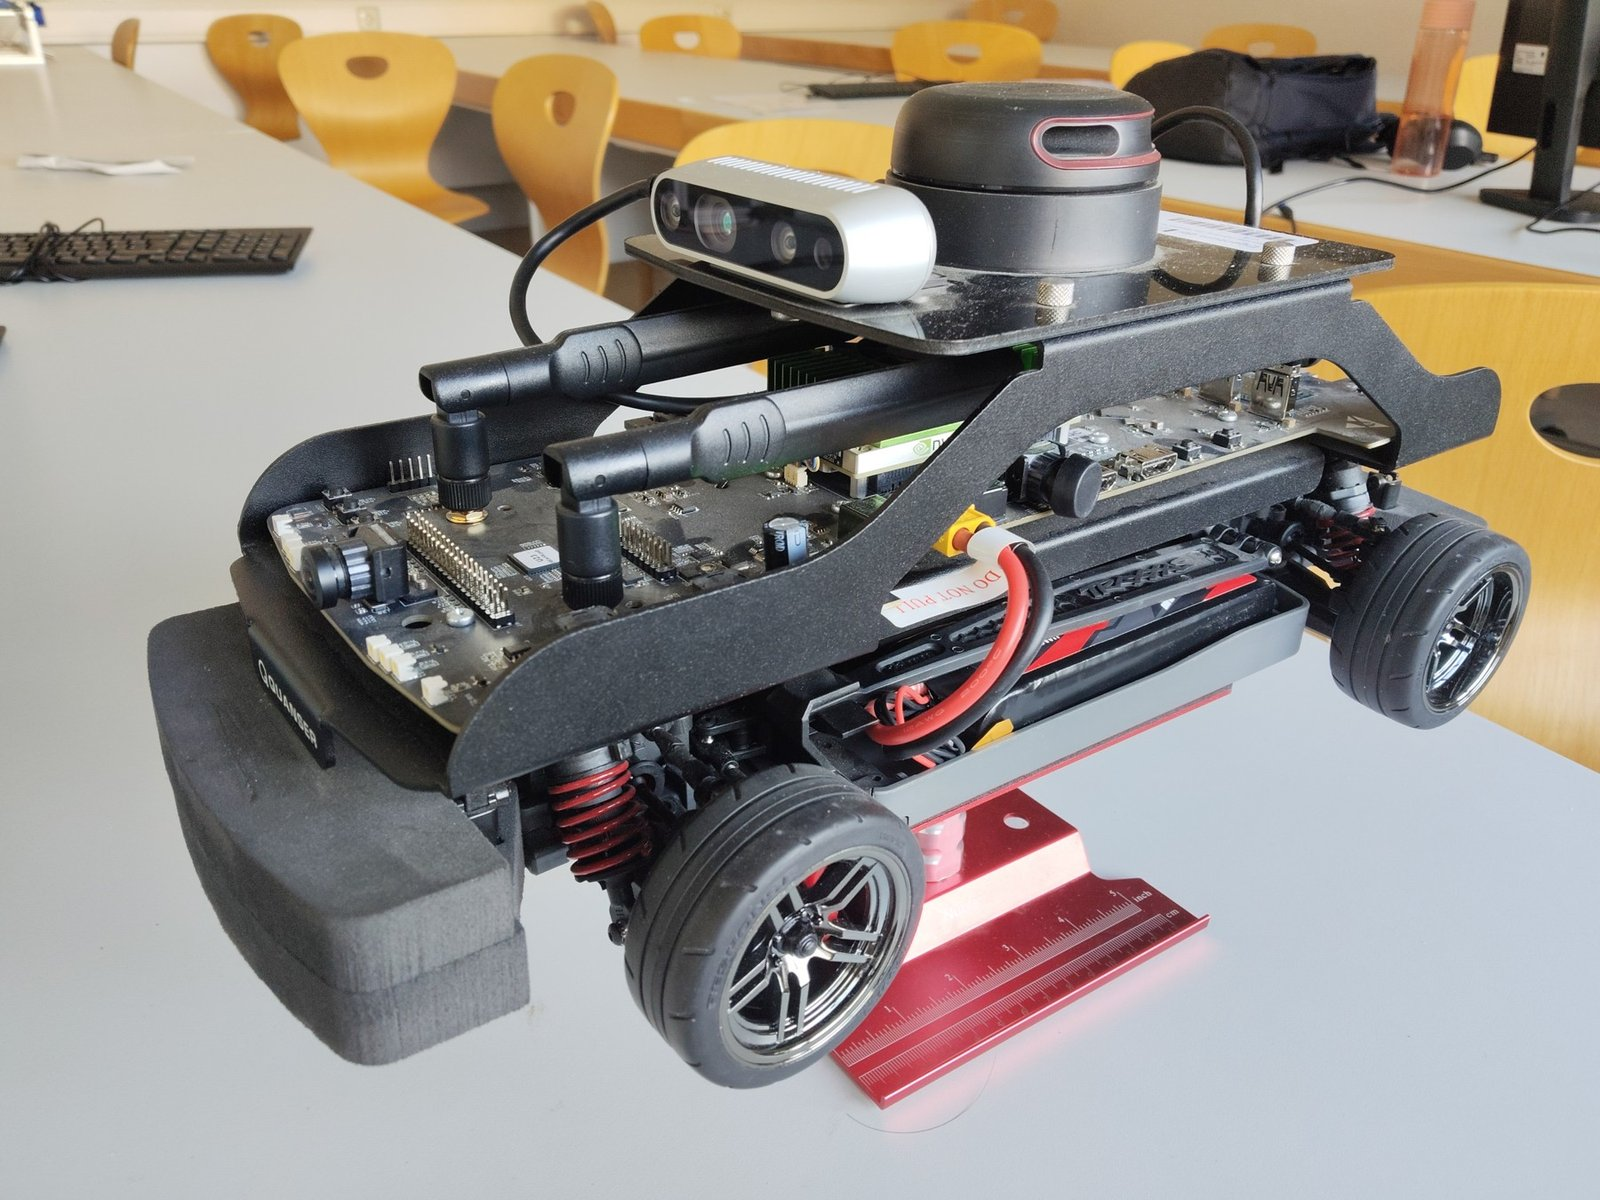
\includegraphics[width=0.75\textwidth]{figures/qcar-sensors-battery-photo.jpg}
  \caption{The Quanser QCar platform used throughout this thesis, raised off the ground.}
  \label{fig:qcar-sensors-battery-photo}
\end{figure}

Drive and steering actuation are exposed through Quanser's own
Hardware Abstraction Layer / Product Application Layer (HAL/PAL)
Python library, which wraps the vehicle's motor, servo, encoder and
battery-monitoring hardware behind a \texttt{QCar} object exposing
\texttt{read()}/\texttt{write()} calls. Two of its limits are enforced
at the field-programmable gate array (FPGA) level regardless of what
software commands \cite{quanser2023qcar}. The steering command range
is $\pm 0.5$~rad against a physical limit of $\pm 0.5236$~rad
($\pm\ang{30}$). An overcurrent protection state, triggered at
5\,A/8\,s, 10\,A/2\,s or 15\,A/0.5\,s, forces the vehicle into a
neutral mode until the underlying hardware-in-the-loop device is
restarted. Both limits are respected throughout every piece of
drive-control code presented in this thesis.

A third figure, commonly listed alongside these two, is not a
hardware-enforced limit at all. Quanser's own troubleshooting
documentation \emph{recommends} saturating commanded PWM duty cycle
to $\pm 30\%$ with a $100\%/\mathrm{s}$ rate limiter, specifically to
avoid a battery-brownout-induced shutdown
\cite{quanser2023troubleshooting} -- not something the HAL itself
clamps. This project's own drive-control code adopts that
recommendation (Section~\ref{sec:final-calibration}'s
\texttt{THROTTLE\_LIMIT}), but it is a software policy choice, not a
property of the vehicle the way the other two limits are.

A property of the HAL library specific to this platform and central
to one of this thesis's most significant findings
(Section~\ref{sec:readmode-bug}) is its two supported I/O modes. In
\emph{immediate I/O} (\texttt{readMode=0}), each call to
\texttt{read()} triggers a fresh hardware sample. In \emph{task-based
I/O} (\texttt{readMode=1}), a background acquisition task begins
sampling into a fixed-depth ring buffer at object construction time,
independently of when (or whether) the caller ever calls
\texttt{read()}. This distinction is not merely an implementation
detail. Chapter~\ref{ch:calibration} documents how it produced a
measurement artefact large enough and stable enough to be
repeatedly and reasonably misattributed to genuine vehicle physics
before its true cause was found.

\section{The Sim-to-Real Gap}
\label{sec:sim-to-real-concept}

The term \emph{sim-to-real gap} (or \emph{reality gap}) is most
extensively studied in the deep-reinforcement-learning literature,
where it refers to the degradation of a policy's performance when a
controller trained purely in simulation is transferred to a physical
robot \cite{zhao2020sim2real}. This thesis borrows the term for a
broader, classically-engineered sense not specific to any learned
policy: any systematic discrepancy between a robot's simulated and
physical behaviour under nominally identical software and commands.
Sources of this gap are commonly grouped into a few broad categories,
all of which recur, in concrete and specific form, across this
thesis's methodology chapters:

\begin{itemize}
  \item \textbf{Unmodelled or under-modelled physical effects} --
    e.g.\ static friction / stiction, actuator response lag or
    non-linear actuator-to-output mappings that a simulator either
    omits entirely or models only in idealised form. Chapter~\ref{ch:calibration}'s
    throttle calibration and friction-deadband findings are a direct
    instance of this category.
  \item \textbf{Sensor and estimation differences} -- simulated
    sensors are frequently noiseless or near-noiseless and
    perfectly time-synchronised with the simulation clock, whereas
    physical sensors carry real noise, real latency and, in a
    distributed system, real inter-process clock skew.
    Chapter~\ref{ch:hardware-bridge}'s clock-offset and LiDAR
    angle-convention fixes fall into this category.
  \item \textbf{Software/communication-layer differences} -- a
    simulated robot typically runs its entire software stack as
    co-located ROS~2 processes on one machine. A physical robot may
    be split across incompatible middleware versions, unreliable
    wireless links or, as found directly in this project, firmware-
   or driver-level buffering that a simulation has no equivalent of
    at all. Chapters~\ref{ch:hardware-bridge}
    and~\ref{ch:calibration} both document findings in this
    category.
\end{itemize}

A methodological point recurs throughout this thesis and is made
explicit here because it shapes every later chapter's approach:
these categories are not always distinguishable from the symptom
alone. A fixed-duration, speed-independent delay between a software
command and its physical effect is, from a black-box measurement
standpoint, equally consistent with several explanations. It could
be drivetrain coasting, a physical-effect explanation or a
command-delivery lag in the bridge software, a communication-layer
explanation. Or, as this thesis's own investigation ultimately
found, it could be a stale-data artefact in a sensor read path -- a
sensor/estimation-layer explanation that happens to mimic a physical
one almost exactly.

Distinguishing between these required, in every case documented in
this thesis, going beyond the symptom to a direct measurement or
source-level inspection of the specific layer under suspicion. This
is a theme Chapter~\ref{ch:calibration} returns to explicitly.

\chapter{Simulation Stack Development}
\label{ch:sim-stack}

% Guideline recommends 10-20 pages per methodology chapter.
% TODO: add figures - a URDF joint-tree diagram, a screenshot of the
% Gazebo model, and an odometry-drift plot from Sec. 3.6 would all
% strengthen this chapter with minimal extra writing.

This chapter documents the development of the simulation-side
navigation stack that Chapters~\ref{ch:hardware-bridge}
through~\ref{ch:nav-integration} later migrate onto physical
hardware. The stack went through two full drive-architecture
migrations before reaching the form used for hardware bridging
(Sections~\ref{sec:baseline-manual}--\ref{sec:second-migration}), and
along the way surfaced a middleware-level parser defect
(Section~\ref{sec:colon-bug}) and a four-part vehicle-dynamics bug
pattern that recurred, largely unchanged, across two sibling packages
(Section~\ref{sec:not-moving-bug}). The chapter closes with a
behaviour-tree fix specific to Ackermann-steered vehicles
(Section~\ref{sec:bt-fix}).

\section{Baseline: Manual Bicycle-Model Inversion}
\label{sec:baseline-manual}

The navigation stack's earliest drive architecture used two
independent \texttt{ros2\_control} \texttt{JointGroup} controllers
(\texttt{drive\_controller} for wheel velocity,
\texttt{steering\_controller} for hub position) driven by a
hand-written node, \texttt{cmd\_vel\_to\_drive.py}, that manually
inverted the bicycle-model relationship of
Equations~\ref{eq:bicycle-x}--\ref{eq:bicycle-theta} to compute a
per-wheel velocity and steering-hub angle from an incoming
\texttt{geometry\_msgs/Twist} on \texttt{/cmd\_vel}. This
architecture worked, but duplicated the Ackermann inverse-kinematics
logic that a purpose-built controller would otherwise provide, and --
more importantly for a navigation stack meant to reach physical
hardware -- could not support Nav2's recovery behaviours that require
reversing, since the manual node had no reverse-driving logic of its
own.

\section{First Migration: \texttt{ros2\_control}'s \texttt{AckermannSteeringController}}
\label{sec:first-migration}

The first architectural migration replaced both custom
\texttt{JointGroup} controllers and \texttt{cmd\_vel\_to\_drive.py}
with \texttt{ros2\_control}'s own
\texttt{ackermann\_steering\_controller} / \texttt{AckermannSteeringController}
plugin, configured via \texttt{config/qcar\_controllers.yaml}. This
controller performs the same Ackermann inverse kinematics internally,
and additionally publishes its own wheel-based odometry -- which
this project deliberately adopted as the vehicle's \texttt{/odom}
source in place of Gazebo's \texttt{gazebo\_ros\_p3d} ground-truth
plugin (the latter was kept running, but remapped to
\texttt{/ground\_truth/odom} for debugging comparison only). This was
a considered choice, not a default: ground-truth odometry is
trivially available in simulation but has no equivalent on the
physical robot, whose odometry can only ever be a real,
drift-prone dead-reckoning estimate (Section~\ref{sec:onboard-bridge-odom}).
Developing and tuning the navigation stack against the same
\emph{kind} of odometry it would have to work with on hardware, from
the start, avoided deferring that discrepancy to the eventual
hardware migration.

Because Nav2, AMCL, and \texttt{bt\_navigator} all hard-code an
expectation that odometry arrives on \texttt{/odom} and driving
commands are consumed from \texttt{/cmd\_vel}, and the new controller
instead exposes these under its own namespaced topics
(\texttt{\textasciitilde/odometry}, \texttt{\textasciitilde/reference\_unstamped}),
two \texttt{topic\_tools relay} nodes were added to the launch files
to bridge the naming mismatch without modifying Nav2 itself.

\subsection{A Wheel-Axis Bug Exposed by the Migration}
\label{sec:wheel-axis-bug}

The migration exposed a latent URDF defect that had been silently
compensated for by the old manual node and had therefore never
produced a visible symptom before. The rear-left drive wheel joint
(\texttt{base\_wheelrl\_joint}) had its \texttt{<origin>} yawed by
\ang{180} for correct mesh mirroring, but retained the \emph{same}
\texttt{<axis>} direction as the corresponding right-side joint --
which, combined with the yaw flip, silently inverted that wheel's
effective rotation sense relative to a positive commanded velocity.
The old \texttt{cmd\_vel\_to\_drive.py} had manually compensated for
this by commanding \texttt{[-speed, +speed]} to the left/right wheel
velocities respectively; the new controller had no such
compensation, and computed wheel odometry that did not match the
vehicle's real motion direction. The fix -- correcting the
\texttt{<axis>} declaration on the affected joint directly, rather
than perpetuating a sign-flip workaround downstream in every
consumer of that joint -- illustrates a pattern worth stating
explicitly: a URDF geometry defect that is silently absorbed by one
consumer's ad hoc compensation will resurface, often with a confusing
symptom, the moment that consumer is replaced.

Listing~\ref{lst:wheel-axis} shows the two rear drive-wheel joints as
they stand in the corrected URDF: the left joint's mesh-mirroring yaw
(\texttt{rpy="0 0 3.14"}) is paired with a negated \texttt{<axis>} so
that a positive commanded wheel velocity turns both wheels in the
same physical sense, whereas the right joint needs no such
compensation since its origin carries no mirroring rotation.

\begin{lstlisting}[language=XML,caption={Rear-left and rear-right drive-wheel joints (\texttt{urdf/qcar\_model.xacro}) -- the axis on the mirrored left joint is negated to compensate for its \ang{180} origin yaw.},label={lst:wheel-axis}]
<joint name="base_wheelrl_joint" type="continuous">
    <parent link="base" />
    <child link="wheelrl" />
    <origin rpy="0 0 3.14" xyz="-0.12765 0.05610 0.03338" />
    <!-- axis negated to compensate for the 180deg yaw above (mesh mirror) -
         without this the left wheel spins opposite the right wheel for the
         same signed velocity command -->
    <axis xyz="0 -1 0" />
</joint>

<joint name="base_wheelrr_joint" type="continuous">
    <parent link="base" />
    <child link="wheelrr" />
    <origin rpy="0 0 0" xyz="-0.12765 -0.05610 0.03338" />
    <axis xyz="0 1 0" />
</joint>
\end{lstlisting}

\paragraph{Why the sign flip happens: axes live in the joint's own, rotated frame.}
The mechanism behind this bug is a direct consequence of one URDF
convention that is easy to overlook: a joint's \texttt{<axis>} vector
is expressed in the joint's \emph{own} local frame -- the frame
produced by applying that same joint's \texttt{<origin>} rotation to
its parent link's frame -- not directly in the parent link's (here,
\texttt{base}'s) frame. The rear-right joint's origin carries no
rotation (\texttt{rpy="0 0 0"}), so its joint frame is identical to
\texttt{base}'s frame, and \texttt{axis="0 1 0"} means exactly
$+Y$ in the vehicle's own reference frame. The rear-left joint's
origin, in contrast, is yawed \ang{180} about $Z$
(\texttt{rpy="0 0 3.14"}) so its mesh renders mirrored on the correct
side of the chassis. A \ang{180} yaw about $Z$ maps a frame's own $X$
and $Y$ axes to their negatives while leaving $Z$ unchanged
($X \to -X$, $Y \to -Y$), so that joint's \emph{local} $+Y$ direction
already points along \emph{base}'s $-Y$ direction before the
\texttt{<axis>} element is even considered. Declaring
\texttt{axis="0 1 0"} on the rear-left joint -- the value that looks,
by simple inspection, like ``the same axis as the right wheel'' --
therefore actually commands rotation about \texttt{base}'s $-Y$, the
opposite physical sense from the right wheel's \texttt{base}-frame
$+Y$, for the identical signed joint velocity. Negating it to
\texttt{axis="0 -1 0"} (Listing~\ref{lst:wheel-axis}) cancels the
already-applied yaw, restoring both wheels to rotating about the same
\texttt{base}-frame axis for the same commanded sign -- the fix is
not ``pick whichever sign makes it drive forward'' by trial and
error, but a direct, derivable consequence of the joint's own origin
rotation, which is why it generalises immediately to any other
mirrored-mesh joint pair in this or a similar URDF.

\subsection{A URDF Parser Defect in \texttt{gazebo\_ros2\_control}}
\label{sec:colon-bug}

While adding explanatory comments to the URDF for the wheel-axis fix
above, \texttt{controller\_manager} began failing to start
altogether -- with all downstream symptoms that implies
(\texttt{joint\_state\_broadcaster} and the new controller never
spawning, \texttt{/odom} never appearing, and no \texttt{map} TF
being published either, since nothing in the chain that would
produce it ever started). The failure was silent: no controller
spawner logged an error explaining \emph{why} it timed out waiting
for \texttt{controller\_manager}.

Isolating the cause required a delta-debugging-style bisection of the
URDF file against the actual parsing code path, since multi-line
comments, apostrophes, and file length were all plausible-looking red
herrings that turned out not to matter. The root cause was found in
how \texttt{gazebo\_ros2\_control} starts its internally-managed
\texttt{controller\_manager} node: the plugin passes the entire
processed URDF as a single \texttt{--param
robot\_description:=<xml>} command-line-style argument, which
\texttt{rcl}'s parameter-override grammar parses looking for a
\texttt{node\_name:param\_name} pattern. That grammar treats
\emph{any} colon immediately followed by a space --
\texttt{": "} -- anywhere in the argument string as a potential
separator, including inside an XML comment that a human reader would
never consider part of the "real" content. A direct reproduction
using \texttt{rclpy}'s own argument parser confirmed the mechanism
precisely: \texttt{"hello: world"} fails to parse while
\texttt{"hello:world"} (no space) succeeds, and \texttt{package://}
URIs or \texttt{foo:=bar} remappings are unaffected since neither
places a bare space directly after a colon.

This is not specific to this project's URDF; it is a property of any
\texttt{gazebo\_ros2\_control}-based setup, and is recorded here as a
general finding: \textbf{a URDF or xacro file must never contain the
literal sequence colon-followed-by-space, including inside comments},
or \texttt{controller\_manager} fails to start with no diagnostic
pointing at the actual cause.

\section{Porting the Navigation Stack to ROS~2 Humble / Gazebo Classic}
\label{sec:humble-conversion}

A sibling package in this project's workspace had been authored
against ROS~2 Jazzy and the newer Gazebo Sim (Harmonic) simulator --
the \texttt{gz sim} binary family, \texttt{ros\_gz\_sim} /
\texttt{ros\_gz\_bridge} integration, and \texttt{gz-sim-*-system}
world plugins -- none of which are available on this project's
ROS~2 Humble / Ubuntu 22.04 / Gazebo Classic~11 host. Rather than
install a second, newer simulator stack alongside the one already
validated and working for the rest of this thesis's packages
(Section~\ref{sec:first-migration}), the package was converted to
Gazebo Classic, matching every other package in this project.
Table~\ref{tab:gz-sim-conversion} summarises the conversion, which
generalises directly to any future package encountered that was
authored against Gazebo Sim / Jazzy-era tutorials.

\begin{table}[htbp]
  \centering
  \caption{Gazebo Sim (Jazzy) to Gazebo Classic (Humble) translation table.}
  \label{tab:gz-sim-conversion}
  \small
  \begin{tabular}{@{}p{4.2cm}p{4.2cm}p{5.5cm}@{}}
    \toprule
    Gazebo Sim (source) & Gazebo Classic (target) & Notes \\
    \midrule
    \texttt{ros\_gz\_sim} / \texttt{ros\_gz\_bridge} (package.xml) & \texttt{gazebo\_ros} / \texttt{gazebo\_plugins} & \\
    \texttt{gpu\_lidar} sensor + gz-sim system plugin & \texttt{type="ray"} + \texttt{\seqsplit{libgazebo\_ros\_ray\_sensor.so}} & \\
    gz-sim \texttt{imu} sensor & classic \texttt{imu} + \texttt{\seqsplit{libgazebo\_ros\_imu\_sensor.so}} & \\
    \texttt{\seqsplit{gz-sim-joint-state-publisher-system}} & removed entirely & Not needed; the drive plugin's own \texttt{publish\_wheel\_tf} broadcasts wheel/steering TF directly \\
    \texttt{\seqsplit{gz-sim-ackermann-steering-system}} & \texttt{\seqsplit{libgazebo\_ros\_ackermann\_drive.so}} & Classic plugin auto-computes wheelbase/track/radius from URDF geometry; the gz-sim system required stating them explicitly \\
    5$\times$ \texttt{<plugin filename="gz-sim-*-system">} (world SDF) & deleted entirely & Classic's \texttt{gzserver} has physics, scene broadcast, and sensors built into its core, not opt-in systems \\
    \texttt{gz sim} + \texttt{ros\_gz\_sim create} spawn + \texttt{ros\_gz\_bridge} node & \texttt{gazebo}/\texttt{gzserver} + \texttt{gazebo\_ros spawn\_entity.py} & No bridge node needed; classic plugins publish onto ROS~2 topics directly \\
    \texttt{GZ\_SIM\_RESOURCE\_PATH} env-var for mesh resolution & not needed & \texttt{gazebo\_ros} registers its own \texttt{package://} resolver \\
    \bottomrule
  \end{tabular}
\end{table}

One element of the original file required \emph{no} change: the
\texttt{<gazebo reference="link">\allowbreak<material>Gazebo/X</material>\allowbreak</gazebo>}
material-script blocks are classic-Gazebo-native syntax that happened
to already be present and compatible, a reminder that a systematic
conversion still benefits from checking each element rather than
assuming every gz-sim-authored construct needs translating.

\section{Second Migration: The Direct Drive Plugin}
\label{sec:second-migration}

The navigation stack's final drive architecture -- the one this
thesis's hardware bridge (Chapter~\ref{ch:hardware-bridge}) targets
-- drops \texttt{ros2\_control} entirely in favour of driving the
robot through \texttt{libgazebo\_ros\_ackermann\_drive.so}\allowbreak{} directly,
declared in a \texttt{<gazebo>} block in the URDF rather than through
a separate controller-manager configuration file, matching the
approach already adopted for the sibling package during the Humble
conversion above. This plugin subscribes to \texttt{/cmd\_vel} and
publishes \texttt{/odom} and the \texttt{odom} $\rightarrow$
\texttt{base} TF transform directly, again auto-computing wheelbase,
track width, and wheel radius from URDF joint and collision geometry
at spawn time -- removing an entire category of configuration
drift risk where a controller's stated geometry parameters could
silently fall out of sync with the URDF's actual geometry, which had
been possible (if not observed) under the first migration's
\texttt{ros2\_control} YAML-based configuration. This is the
architecture described in Section~\ref{sec:gazebo}'s account of the
drive plugin, and the one whose real-world calibration
Chapter~\ref{ch:calibration} presents.

\subsection{A Quiet Regression: Odometry Reverts to Ground Truth}
\label{sec:odom-regression}

This migration has one consequence worth stating explicitly, because
it is easy to overlook and was not caught at the time: it silently
reversed the odometry-source decision made in
Section~\ref{sec:first-migration}. Reading
\texttt{gazebo\_ros\_ackermann\_drive}'s own
\texttt{UpdateOdometryWorld()} implementation directly shows that its
\texttt{/odom} is computed from \texttt{model\_->WorldPose()} and
\texttt{model\_->WorldLinearVel()} -- the physics engine's own exact,
noise-free simulated pose and velocity for the whole vehicle body --
not an integration of individual wheel-joint velocities or steering
angles at all. In other words, the final simulation-side drive
architecture publishes \texttt{/odom} that is, mechanically, no
different from what \texttt{gazebo\_ros\_p3d} (Section~\ref{sec:first-migration})
would have provided: perfect, driftless ground truth, despite carrying
the same topic name and message type the first migration deliberately
chose \emph{instead of} ground truth.

This is not a bug in the sense the rest of this chapter uses the
word -- the plugin behaves exactly as its own source dictates, and
nothing in this project's testing depended on \texttt{/odom} actually
drifting in simulation. It is, however, a genuine and previously
unrecorded discrepancy between this thesis's stated intent (train
against the same \emph{kind} of odometry the physical robot will
have) and what the final simulation configuration actually exercises,
and it is worth stating plainly rather than leaving the earlier
claim uncorrected: \textbf{only the physical QCar's own odometry
(Chapter~\ref{ch:hardware-bridge}, Section~\ref{sec:onboard-bridge-odom})
is genuine encoder-based dead reckoning in this project; the
simulation's final \texttt{/odom} is ground truth, exactly like the
\texttt{gazebo\_ros\_p3d} source it was originally meant to replace}.
Framed in terms of Section~\ref{sec:sim-to-real-concept}'s sim-to-real
gap taxonomy, this means the localisation/odometry accuracy gap
between simulation and hardware in this project is not purely an
empirically discovered discrepancy -- it is, in part, structurally
guaranteed by this architecture, since the simulated AMCL/Nav2 stack
is given a perfect motion estimate that its real-hardware counterpart
can never have. Any future comparison of localisation accuracy
between simulation and hardware should account for this rather than
treating the two \texttt{/odom} streams as like for like.

\section{The ``Robot Not Moving Forward'' Bug Pattern}
\label{sec:not-moving-bug}

Both the sibling package's Humble conversion (Section~\ref{sec:humble-conversion})
and this project's own second migration (Section~\ref{sec:second-migration})
independently produced the same surface symptom immediately
afterward: the simulated vehicle did not drive forward under a
sustained \texttt{/cmd\_vel} command. In both cases, this single
symptom turned out to be caused by a stack of independent bugs, each
one masking the next until the previous was fixed -- a pattern
significant enough, and confirmed to recur closely enough between
the two packages, to warrant treating as a general defect signature
for this plugin/vehicle combination rather than two unrelated
incidents. Table~\ref{tab:not-moving-bugs} summarises all bugs found
across both occurrences.

\begin{table}[htbp]
  \centering
  \caption{The recurring ``not moving forward'' bug pattern, as found in both affected packages.}
  \label{tab:not-moving-bugs}
  \small
  \begin{tabular}{@{}p{0.6cm}p{5.3cm}p{7cm}@{}}
    \toprule
    \# & Bug & Symptom / mechanism \\
    \midrule
    1 & Wheel \texttt{<collision>} was the visual STL mesh, not a primitive shape & The plugin's radius auto-detection only supports cylinder/sphere collisions; a mesh collision silently returns radius 0, so \texttt{target\_linear / wheel\_radius} becomes infinite, poisoning the velocity PID regardless of gain. Fixed by keeping the STL for \texttt{<visual>} but using an explicit \texttt{<cylinder radius="0.036" length="0.0245"/>} for \texttt{<collision>}. \\
    2 & Zero Coulomb friction on the wheel links & Even with a correct wheel radius, the wheel spins at exactly the commanded angular velocity forever while the chassis never translates -- 100\% slip. Fixed with \texttt{<mu1>1.0</mu1><mu2>1.0</mu2>} on every wheel link. \\
    3 & Absurd ground-plane friction (\texttt{mu=100}, \texttt{mu2=50}) & Once wheel friction is fixed, this combination produces a real physics instability/NaN blow-up on contact. Fixed by lowering to a realistic \texttt{mu=1}, \texttt{mu2=1}. \\
    4 & Razor-thin wheel/ground clearance (only $\sim$0.38\,mm geometric overlap at the original 0.033\,m collision radius) & Enough overlap to rest on the ground without falling through, but not enough consistent contact-normal force to generate real traction even at correct friction -- chassis twist stayed near zero despite full wheel spin. Fixed by padding the collision cylinder radius to 0.036\,m (+3\,mm), which alone flipped the vehicle from ``spins in place'' to sustained forward motion. \\
    \bottomrule
  \end{tabular}
\end{table}

Listing~\ref{lst:wheel-collision-friction} shows the corrected form of
one rear wheel link and its friction declaration, combining the fixes
for bugs~1 and~2 from Table~\ref{tab:not-moving-bugs}: an explicit
cylinder \texttt{<collision>} geometry (the \texttt{<visual>} mesh,
omitted here, is unaffected and keeps using the STL), and a separate
\texttt{<gazebo reference="...">} block assigning Coulomb friction
coefficients to that same link -- URDF has no wheel-friction concept
of its own, so this Gazebo-specific extension is the only place that
value is set at all.

\begin{lstlisting}[language=XML,caption={Wheel collision cylinder and friction (\texttt{urdf/qcar\_model.xacro}) -- fixes for bugs 1 and 2 in Table~\ref{tab:not-moving-bugs}.},label={lst:wheel-collision-friction}]
<link name="wheelrl">
    <collision>
        <origin rpy="1.5708 0 0" xyz="0 0 0" />
        <geometry>
            <cylinder radius="0.036" length="0.0245" />
        </geometry>
    </collision>
    <!-- <visual> (STL mesh) and <inertial> omitted here, unaffected -->
</link>

<!-- wheel-ground friction - without this the wheels spin freely with 100%
     slip and the chassis never translates, regardless of PID gains -->
<gazebo reference="wheelrl">
    <mu1>1.0</mu1>
    <mu2>1.0</mu2>
</gazebo>
\end{lstlisting}

\paragraph{Mechanism: how bugs 1 and 2 poison the control loop and physics, in numbers.}
Section~\ref{sec:gazebo-pid-loop} and Section~\ref{sec:friction-theory}
give the general theory bugs~1 and~2 exercise; concretely, for this
vehicle, a commanded \SI{0.3}{\meter\per\second} with a mesh-shaped
(bug~1, radius $\to 0$) rear-wheel collision computes a target angular
velocity of $0.3 / 0 \to \infty$ rad/s in
Equation~\ref{eq:pid}'s error term -- not a large but finite number
that a differently-tuned PID could still track, but a value with no
finite representation at all, driving the linear-velocity PID's
output straight to its saturation limit on the very first physics
step regardless of gain. With the corrected \SI{0.036}{\meter} radius
(Listing~\ref{lst:wheel-collision-friction}) that same command instead
computes a finite target of $0.3 / 0.036 \approx \SI{8.33}{\radian\per\second}$,
a well-posed, trackable error signal. Bug~2 (zero friction) then
governs whether that correctly-spinning wheel produces any chassis
motion at all: with $\mu_1 = \mu_2 = 0$, Section~\ref{sec:friction-theory}'s
Coulomb limit permits zero tangential contact force regardless of how
much normal force the vehicle's weight presses the wheel into the
ground with, so the wheel can spin at exactly the commanded
\SI{8.33}{\radian\per\second} indefinitely while contributing zero
net force to the chassis -- the two bugs therefore fail at two
different, independently necessary conditions (a well-posed control
error, and a nonzero force limit to actually convert correct wheel
spin into chassis thrust), which is why fixing either one alone still
left the vehicle stationary and only fixing both together produced
motion.

The first occurrence of this pattern also included a preceding, more
basic defect specific to that package: its mesh URIs
(\texttt{package://.../models/qcar/QCarBody.stl}-style paths) pointed
at a directory layout copy-pasted from this project's own package
rather than the sibling's actual \texttt{meshes/} layout and file
names, so the robot had \emph{no} collision geometry at all and fell
through the simulated ground plane -- confirmed directly via
\texttt{/odom} tracking a $z$-position reaching approximately
$-38{,}000$\,m. This is worth recording as a separate, more
fundamental lesson: Gazebo Classic's URDF-to-SDF loader silently
rewrites \texttt{package://} mesh URIs to \texttt{model://}, which
only resolves via the \texttt{GAZEBO\_MODEL\_PATH} environment
variable -- and since neither package's \texttt{package.xml} exports
the \texttt{<gazebo\_ros gazebo\_model\_path=.../>} tag required for
that resolution, correcting the path string alone would not have
been sufficient. The fix instead used xacro's \texttt{\$(find)}
substitution to build \texttt{file://} URIs directly, which bypass
package-path resolution entirely.

The second occurrence additionally required a numerical-stability
fix not initially anticipated: wheel rotational inertia values that
were physically correct for a solid disk of the wheel's real mass and
radius, but small enough in absolute terms to interact badly with the
plugin's 100\,Hz PID control loop, producing an
\texttt{Ogre::AxisAlignedBox::setExtents} assertion crash a few
seconds into driving. Bumping wheel inertia roughly 20$\times$
(\texttt{ixx=izz=0.0012}, \texttt{iyy=0.0022}) together with lowering
the steering and linear-velocity PID gains resolved the crash; this
value combination, once found working in the first occurrence, was
reused directly in the second and confirmed stable there as well.

A further gain-tuning finding, specific to the second occurrence and
worth stating as a general caution for reusing PID values across
otherwise-identical vehicle configurations: a steering PID gain
verified stable and accurate on a \emph{frictionless} wheel
configuration produced a real turning radius roughly $6\times$ larger
than commanded once realistic wheel friction (bug~2 above) was added,
because the same low gain that was previously sufficient (with no
resistive torque to overcome) could no longer turn the front hubs
against a now-gripping, rolling tyre. The fix -- raising
\texttt{left/right\_steering\_pid\_gain} from \texttt{0.02} to
\texttt{3.0} -- was verified directly via TF lookups on the
steering-hub joints during a commanded 1.0\,m-radius turn, confirming
hub angles converging to the correct $\sim$\ang{15}--\ang{18}
Ackermann inner/outer split, and via a circle fit to the resulting
odometry trace, which recovered a turning radius of 0.87\,m against
the 1.0\,m commanded -- a reasonable margin given the real-vs-ideal
gap between the single-track model of
Section~\ref{sec:ackermann-kinematics} and the vehicle's true
four-wheel geometry.

\subsection{Diagnostic Method}
\label{sec:diagnostic-method}

A methodological point generalises from both occurrences of this bug
pattern: none of these four bugs are visible from \texttt{ros2 topic
list} or a static inspection of the URDF alone. A simulated robot
that appears correctly configured can simultaneously be in freefall,
frozen inside a crashed-but-still-running \texttt{gzserver} process,
or driving its wheels at 100\% slip with zero real chassis motion --
and none of these states are distinguishable without directly
comparing \texttt{/odom} position over several seconds of sustained
commanded motion, cross-checked against the Gazebo server log for
silent \texttt{[Err]}/assertion lines. This became this project's
standard verification method for any subsequent URDF or physics
change to the simulation stack.

\section{A Behaviour-Tree Fix for Ackermann Recovery}
\label{sec:bt-fix}

\paragraph{How a behaviour tree actually executes.}
A behaviour tree is evaluated by repeatedly ``ticking'' it from the
root: each tick propagates down the tree and every node it reaches
returns one of \texttt{SUCCESS}, \texttt{FAILURE}, or
\texttt{RUNNING} (still in progress, re-tick next cycle) back up to
its parent, and how a parent node interprets its children's results
depends entirely on that parent's type. A \texttt{RoundRobin} node --
the one this section's fix concerns -- ticks exactly one of its
children per activation (advancing to the next child, wrapping back
to the first, only once the currently-selected child itself returns
\texttt{SUCCESS} or \texttt{FAILURE} rather than \texttt{RUNNING}),
cycling through its full child list one at a time across repeated
recovery attempts rather than trying all of them on a single
activation. A \texttt{ReactiveFallback} (the parent of
\texttt{RecoveryActions} in Listing~\ref{lst:bt-recovery}) instead
re-ticks its children from the first one every single tick, moving on
to the next only if the current one fails -- the two control-flow
types are not interchangeable, and Nav2's stock recovery subtree pairs
them deliberately: the outer \texttt{ReactiveFallback} re-checks
whether a goal update has arrived (via the \texttt{GoalUpdated}
condition node) before committing to whichever recovery action the
inner \texttt{RoundRobin} has advanced to.

A separate, functional (rather than purely physics-level) issue
appeared once the vehicle was reliably driving: Nav2's default
recovery behaviour tree round-robins through
\texttt{[ClearCostmaps, Spin(1.57\,rad), Wait(5\,s), BackUp(0.3\,m)]}
whenever the active controller reports it cannot make further
progress. The \texttt{Spin} recovery commands a pure in-place
rotation -- physically impossible for an Ackermann-steered vehicle,
whose steering angle has no effect while linear velocity is zero, so
the vehicle simply cannot rotate without also translating. Roughly
one in three recovery attempts was therefore a guaranteed no-op that
burned its full timeout without attempting any corrective motion.

The fix was to remove \texttt{<Spin>} from the recovery action list
in local copies of Nav2's stock behaviour-tree XML files
(\texttt{navigate\_to\_pose\_w\_replanning\_and\_recovery.xml} and
its through-poses equivalent), wired into the launch configuration
via a \texttt{RewrittenYaml} substitution. This required one
non-obvious step: \texttt{RewrittenYaml} only overwrites
\emph{existing} leaf keys in a YAML file, it does not add new ones,
so the parameter keys pointing at these custom BT file paths
(\texttt{default\_nav\_to\_pose\_bt\_xml} /
\texttt{default\_nav\_through\_poses\_bt\_xml}) had to already exist
as placeholder entries in \texttt{nav2\_params.yaml} before the
launch-time substitution could take effect.

Listing~\ref{lst:bt-recovery} shows the resulting recovery fallback
from the local behaviour-tree copy: a \texttt{RoundRobin} of clearing
both costmaps, waiting, and backing up -- with no \texttt{<Spin>}
node present at all, compared to the stock tree's four-way rotation
through \texttt{[ClearCostmaps, Spin, Wait, BackUp]}.

\begin{lstlisting}[language=XML,caption={Recovery actions in the local behaviour-tree copy (\texttt{config/nav2/behavior\_trees/navigate\_to\_pose\_w\_replanning\_and\_recovery.xml}) -- no \texttt{<Spin>} node, unlike the Nav2 stock tree.},label={lst:bt-recovery}]
<ReactiveFallback name="RecoveryFallback">
  <GoalUpdated/>
  <RoundRobin name="RecoveryActions">
    <Sequence name="ClearingActions">
      <ClearEntireCostmap name="ClearLocalCostmap-Subtree"
        service_name="local_costmap/clear_entirely_local_costmap"/>
      <ClearEntireCostmap name="ClearGlobalCostmap-Subtree"
        service_name="global_costmap/clear_entirely_global_costmap"/>
    </Sequence>
    <Wait wait_duration="5"/>
    <BackUp backup_dist="0.30" backup_speed="0.05"/>
  </RoundRobin>
</ReactiveFallback>
\end{lstlisting}

Because \texttt{RoundRobin} advances exactly one position per
activation, dropping \texttt{Spin} from a four-child list to this
three-child list is not merely ``the useless action happens less
often'' -- it removes the guaranteed no-op activation entirely, so
every single recovery activation now attempts a physically achievable
action, and the cycle back to any one specific action (e.g.\ back to
\texttt{BackUp} after it was last tried) also completes one activation
sooner than it did with four children in the rotation.

\section{Summary of the Simulation-Stack Architecture}
\label{sec:sim-stack-summary}

By the end of this chapter's work, the simulation-side navigation
stack consists of: a URDF-described vehicle driven directly by
\texttt{libgazebo\_ros\_ackermann\_drive.so} (Section~\ref{sec:second-migration}),
publishing ground-truth-derived \texttt{/odom} (Section~\ref{sec:odom-regression}
-- a quiet regression from the genuine dead-reckoning odometry the
first migration, Section~\ref{sec:first-migration}, had deliberately
adopted), with corrected wheel collision geometry, friction, and inertia
(Section~\ref{sec:not-moving-bug}), tuned PID gains for both drive
and steering, and a custom Ackermann-aware recovery behaviour tree
(Section~\ref{sec:bt-fix}). This is the configuration
Chapter~\ref{ch:hardware-bridge} treats as the reference to be
matched -- as closely as the physical robot's own constraints allow
-- when bridging to hardware.

\chapter{Real-Hardware Bridge Architecture}
\label{ch:hardware-bridge}

This chapter presents the architecture built to connect the
simulation-validated navigation stack of Chapter~\ref{ch:sim-stack}
to the physical QCar. Section~\ref{sec:rmw-incompatibility}
establishes why native ROS~2 communication with the robot's onboard
compute is not available, which motivates the TCP/JSON bridge
architecture of Section~\ref{sec:bridge-architecture}. The remaining
sections document the sensor and actuator correctness issues found
while bringing that bridge up to the same fidelity as the simulation
stack: LiDAR angle convention (Section~\ref{sec:lidar-angle}),
odometry (Section~\ref{sec:onboard-bridge-odom}), steering trim
(Section~\ref{sec:steering-trim}) and inter-machine clock
synchronisation (Section~\ref{sec:clock-offset}).

\section{Why Native ROS~2 Communication With the QCar Is Not Available}
\label{sec:rmw-incompatibility}

Two separate constraints rule out installing ROS~2 Humble directly
on the QCar's own compute. Either one alone would have forced the
bridge architecture of Section~\ref{sec:bridge-architecture}.
Together, they leave no realistic native alternative.

\paragraph{Storage.}
As described in Section~\ref{sec:qcar-platform}, the Jetson TX2's
32\,GB eMMC \cite{quanser2023qcar} already carries Ubuntu 18.04, ROS~1 Melodic, ROS~2
Dashing and Quanser's own HAL/PAL software. A second, full ROS~2
Humble installation needs its own client libraries, its own DDS
implementation and driver code to bridge ROS~2 to the HAL/PAL
layer. Fitting all of that into what remained of the 32\,GB was
judged unlikely, based on the typical size of a ROS~2 Humble
install. This constraint does not depend on whether Dashing and
Humble can otherwise talk to each other. Fixing DDS compatibility
would not, by itself, free up disk space.

\paragraph{The ROS~2 Dashing / Humble DDS Incompatibility.}
Independently of storage, this incompatibility was tested directly
rather than assumed. The QCar's onboard Jetson TX2 ships with ROS~2
Dashing (released 2019) pre-installed, while this project's
navigation stack targets ROS~2 Humble (released 2022). Section~\ref{sec:ros2-model}
established that ROS~2 nodes communicate via DDS participants that
must share a compatible discovery and wire protocol to find each
other at all. The working hypothesis at the start of this thesis's
hardware phase was that this would be a soft compatibility problem:
degraded performance, perhaps, but not a hard failure.

A minimal ROS~2 publisher (\texttt{demo\_nodes\_cpp talker}) on the
QCar and a minimal subscriber (\texttt{demo\_nodes\_py listener}) on
the development PC, both configured with the same
\texttt{ROS\_DOMAIN\_ID}, never established communication across
three repeated attempts. The talker was independently confirmed to
be actively publishing each time. The network layer itself was
systematically ruled out before concluding this was a
middleware-level problem. Raw UDP unicast passed cleanly in both
directions, including on the exact Fast~DDS discovery port for the
domain in use. No firewall was active on either host. An
explicit unicast-peers Fast~DDS XML profile, which bypasses
multicast-based discovery entirely, still failed to achieve
discovery. This isolates the failure to the DDS protocol
implementation itself: a genuine Fast~DDS protocol-version
incompatibility between the versions bundled with ROS~2 Dashing and
ROS~2 Humble respectively. Each RTPS message identifies the protocol
version its sender implements \cite{omg2014rtps}. Two peers
implementing different versions can fail to complete discovery even
when the underlying network path is sound. This is not a network,
firewall, or configuration problem that could be worked around
within ROS~2 itself.

This result rules out one further option that the storage constraint
alone would not: running a Humble-compatible container on the QCar
instead of a second native install. A Humble Docker container was
considered early on. It only partially sidesteps the storage
question: a container image adds its own storage overhead rather
than removing it. Nor does it address the protocol-version
incompatibility at the DDS transport layer at all.
The Dashing side of the link is fixed by what physically runs on the
vehicle's ROS~2 partition and cannot itself be upgraded without
departing from the vendor-supported software image.

\section{Bridge Architecture Overview}
\label{sec:bridge-architecture}

\begin{figure}[htbp]
  \centering
  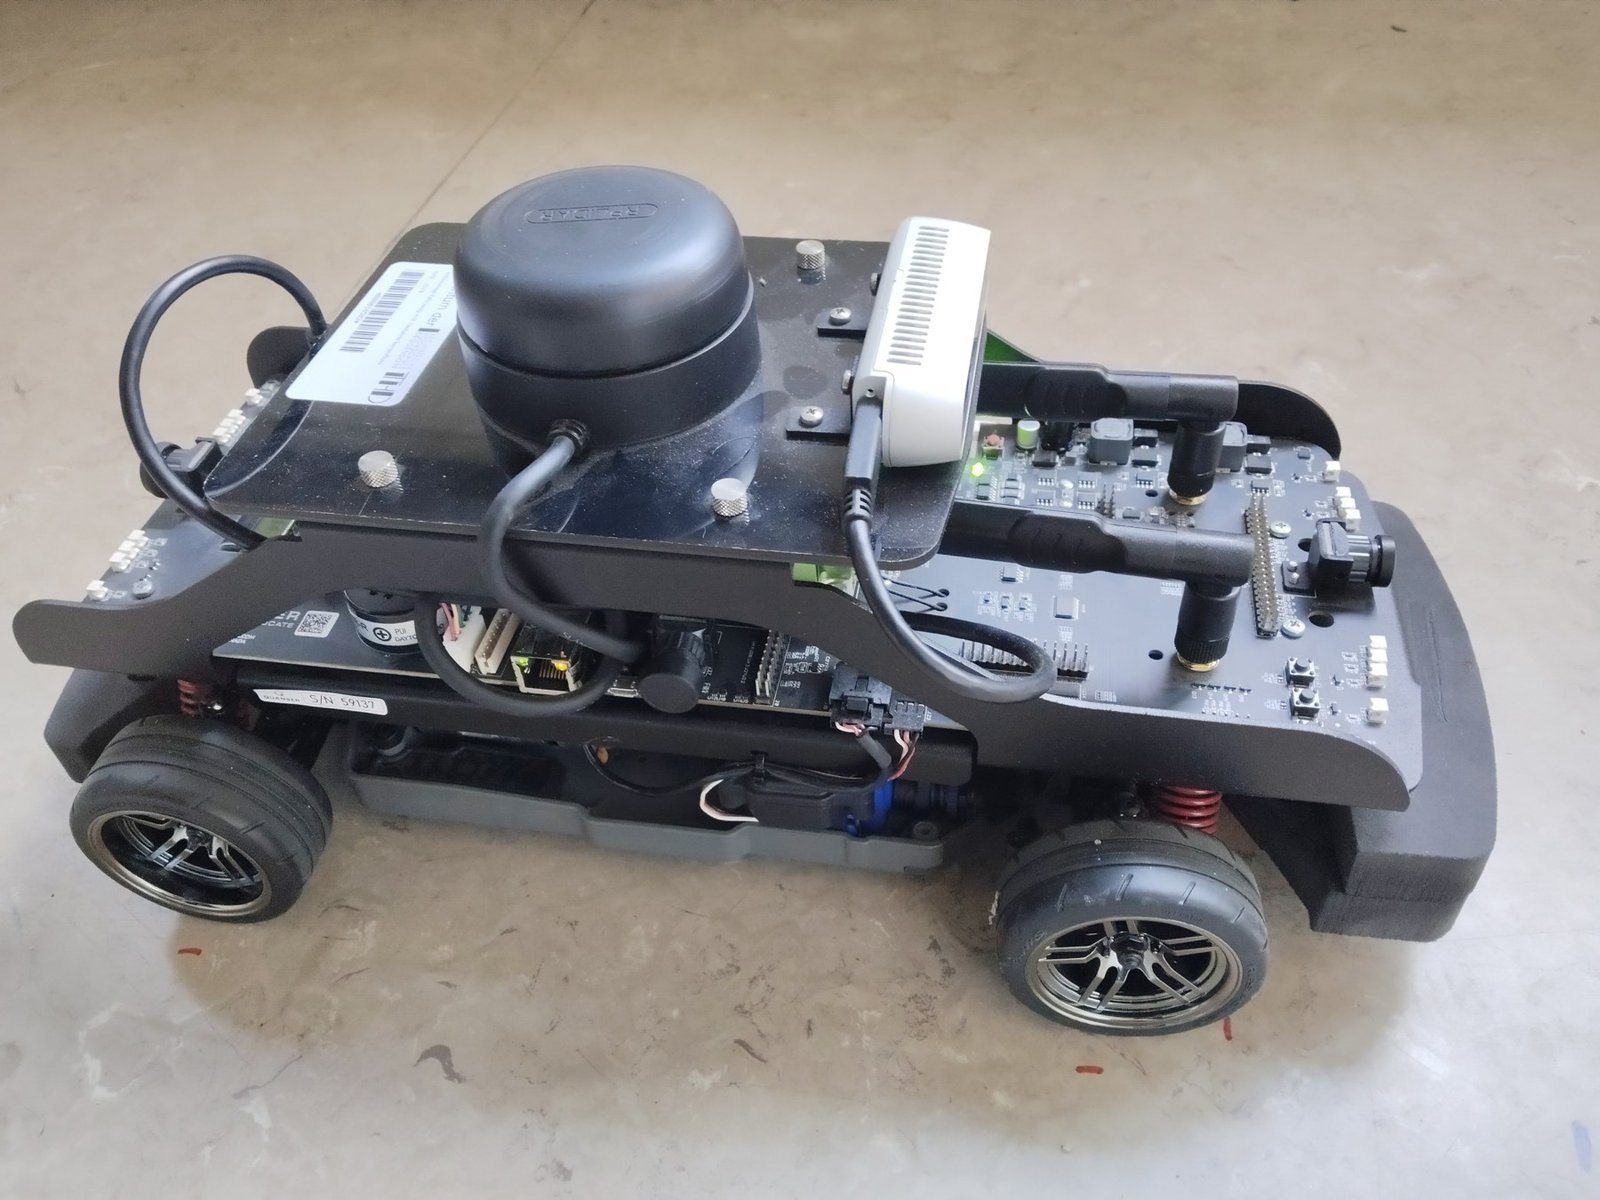
\includegraphics[width=0.75\textwidth]{figures/qcar-compute-sideview-photo.jpg}
  \caption[Side view of the QCar's onboard compute stack]{A side view of the physical QCar showing the onboard
    compute and sensing stack that this bridge architecture runs on:
    the RPLiDAR unit, the Jetson TX2 carrier board (with its wireless
    antennas and USB peripherals) and the wireless router used for
    the development PC's network link, all mounted above the chassis
    and drivetrain.}
  \label{fig:qcar-compute-sideview-photo}
\end{figure}

The architecture built in response uses no ROS~2 at all on the
QCar's own compute. Two plain Python processes run directly on the
Jetson TX2 (no \texttt{colcon} build, invoked as
\texttt{python3 <script>.py}):

\begin{itemize}
  \item \texttt{qcar\_bridge.py} -- a TCP server (port 5555) wrapping
    the Quanser HAL/PAL \texttt{QCar} object (Section~\ref{sec:qcar-platform}):
    receives newline-delimited JSON drive/steering commands and
    responds with odometry JSON over the same full-duplex connection.
  \item \texttt{qcar\_lidar\_node.py} -- a second TCP server (port
    5556) wrapping the LiDAR driver, streaming scan data as
    newline-delimited JSON.
\end{itemize}

On the development PC, a single node, \texttt{qcar\_relay\_node.py},
is the sole point of contact between ROS~2 and this TCP/JSON
protocol. It subscribes to \texttt{/cmd\_vel} and forwards commands
into the motor socket. The same node also publishes \texttt{sensor\_msgs/LaserScan}
on \texttt{/scan} and \texttt{nav\_msgs/Odometry} plus the
\texttt{odom} $\rightarrow$ \texttt{base} TF on \texttt{/odom}, from
data received back over both sockets. Every other node in the
navigation stack -- Nav2, AMCL, Cartographer, RViz -- interacts with
this relay node exactly as it would with the simulation's own drive
plugin. This requires no awareness that the underlying vehicle is real
hardware reached over a bespoke protocol rather than a co-located
Gazebo simulation.

Listing~\ref{lst:bridge-recv-loop} shows the command-receiving side of
this protocol inside \texttt{qcar\_bridge.py}'s main loop: incoming
TCP bytes are accumulated into a buffer and split on newlines. Each
complete line is then parsed as one JSON object, while a malformed
line is logged and discarded rather than allowed to crash the control loop.
This is deliberately fail-soft, since this loop is also driving the
physical motor and must keep running even if one message is corrupt.

\begin{lstlisting}[language=Python,caption={Newline-delimited JSON command parsing inside \texttt{qcar\_bridge.py}'s main loop.},label={lst:bridge-recv-loop}]
chunk = conn.recv(4096)
if chunk == b'':
    print('dev PC relay disconnected')
    break
buf += chunk
while b'\n' in buf:
    line, buf = buf.split(b'\n', 1)
    if not line.strip():
        continue
    try:
        cmd = json.loads(line)
        target_linear = float(cmd['linear_x'])
        angular_z = float(cmd['angular_z'])
        target_steering = compute_steering(target_linear, angular_z)
        last_cmd_time = time.time()
    except (ValueError, KeyError, TypeError):
        print('bad command line, ignoring:', line)
\end{lstlisting}

\paragraph{Why TCP, why newline-delimited JSON and why one socket per direction.}
Three protocol design choices underlie Listing~\ref{lst:bridge-recv-loop}
and are worth making explicit, since each addresses a specific
failure mode rather than being an arbitrary convenience. \textbf{TCP rather than UDP}: TCP guarantees in-order, complete
delivery of every byte sent (retransmitting silently on packet loss)
at the cost of unbounded, variable latency under loss, whereas UDP
offers low, predictable latency but silently drops or reorders
packets under loss with no delivery guarantee at all
\cite{rfc793tcp,rfc768udp}. For velocity
and steering commands, a stale duplicate or a dropped byte silently
corrupting the JSON stream is a worse failure than an occasional
extra tens of milliseconds of latency -- latency that the
\texttt{CMD\_TIMEOUT} watchdog in Section~\ref{sec:onboard-bridge-odom}
already treats as a safety condition regardless of its cause. TCP's
reliability guarantee won out over UDP's
lower-latency-but-lossy profile.

\textbf{Newline-delimited JSON rather than a fixed-length or
length-prefixed binary framing}: TCP is a byte stream with no
built-in concept of message boundaries, so \emph{some} framing scheme
is unavoidable. A length-prefixed binary format would be marginally
more compact, but a plain ASCII delimiter is trivially inspectable
with a bare \texttt{nc}/\texttt{telnet} session during debugging.
This was a real, exercised advantage throughout this project's
development, not a theoretical one. A plain delimiter also requires
no shared binary schema to keep in sync between the QCar-side Python
and dev-PC-side Python.

This is also why \texttt{buf} accumulates across \texttt{recv()}
calls, rather than assuming one \texttt{recv()} returns exactly one
message. TCP's byte-stream semantics make no guarantee that message
boundaries align with any particular \texttt{recv()} call's return:
a message can legitimately arrive split across two calls, or two
messages can arrive concatenated in one call.
Listing~\ref{lst:bridge-recv-loop}'s \texttt{while b'\textbackslash n' in buf}
loop handles both cases uniformly, by always operating on whatever
has accumulated so far.

\textbf{One full-duplex socket carrying both directions},
rather than two separate one-way sockets for commands and odometry:
a single TCP connection is inherently bidirectional, since each
endpoint can read and write independently on the same socket.
Section~\ref{sec:onboard-bridge-odom}'s later addition of odometry
sent back to the relay required no new listening port or
connection -- only using a direction of the existing socket that
had, until then, been opened but left unread.

Figure~\ref{fig:bridge-architecture} shows the complete command and
sensor data path across both machines and both TCP sockets, matching
exactly the components and topics named above.

\begin{figure}[htbp]
  \centering
  \resizebox{\textwidth}{!}{%
  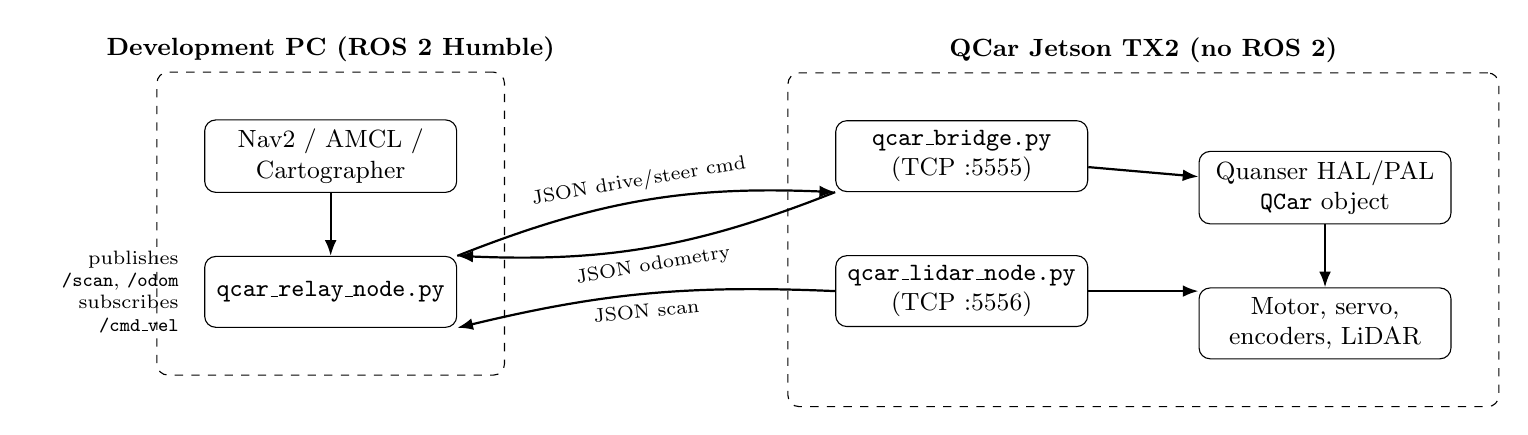
\begin{tikzpicture}[
      node distance=8mm and 14mm,
      box/.style={draw, rounded corners, align=center, minimum height=9mm,
        minimum width=32mm, font=\small},
      hostbox/.style={draw, dashed, inner sep=6mm, rounded corners},
      lbl/.style={font=\scriptsize, align=center},
      arr/.style={-{Latex[length=2mm]}, thick}
    ]

    % --- Development PC (ROS 2 Humble side) ---
    \node[box] (nav2) {Nav2 / AMCL /\\Cartographer};
    \node[box, below=of nav2] (relay) {\texttt{qcar\_relay\_node.py}};
    \node[lbl, left=2mm of relay, align=right, text width=18mm]
      {publishes\\\texttt{/scan}, \texttt{/odom}\\subscribes\\\texttt{/cmd\_vel}};

    \node[hostbox, fit=(nav2)(relay), label={[font=\small\bfseries]above:Development PC (ROS~2 Humble)}] (pcbox) {};

    % --- QCar Jetson TX2 (no ROS 2) ---
    \node[box, right=48mm of nav2] (bridge) {\texttt{qcar\_bridge.py}\\(TCP :5555)};
    \node[box, below=of bridge] (lidarnode) {\texttt{qcar\_lidar\_node.py}\\(TCP :5556)};
    \node[box, right=of bridge, yshift=-4mm] (hal) {Quanser HAL/PAL\\\texttt{QCar} object};
    \node[box, below=of hal] (motor) {Motor, servo,\\encoders, LiDAR};

    \node[hostbox, fit=(bridge)(lidarnode)(hal)(motor), label={[font=\small\bfseries]above:QCar Jetson TX2 (no ROS~2)}] (qcarbox) {};

    % --- Vertical flow inside each host ---
    \draw[arr] (nav2) -- (relay);
    \draw[arr] (bridge) -- (hal);
    \draw[arr] (lidarnode.east) -- (hal.west |- lidarnode.east);
    \draw[arr] (hal) -- (motor);

    % --- Cross-machine TCP/JSON links ---
    \draw[arr] (relay.north east) to[bend left=12]
      node[lbl, above, sloped]{JSON drive/steer cmd}
      (bridge.south west);
    \draw[arr] (bridge.south west) to[bend left=12]
      node[lbl, below, sloped]{JSON odometry}
      (relay.north east);
    \draw[arr] (lidarnode.west) to[bend right=8]
      node[lbl, below, sloped]{JSON scan}
      (relay.south east);

  \end{tikzpicture}%
  }
  \caption[Command/sensor data path: Nav2 to physical actuators]{Command and sensor data path from the Nav2 stack to the
    physical actuators and back. Both cross-machine links are
    newline-delimited JSON over TCP (ports 5555 and 5556); no ROS~2
    process runs on the QCar's own compute at any point in this
    path.}
  \label{fig:bridge-architecture}
\end{figure}

Both onboard TCP servers were built to handle \texttt{SIGTERM}
identically to \texttt{SIGINT} -- a deliberate correctness fix, not
a default. Python does not automatically translate a plain
\texttt{pkill}'s default \texttt{SIGTERM} into a caught, clean-exit
signal the way it does for \texttt{SIGINT} (Ctrl-C). An earlier
plain \texttt{pkill} against the LiDAR process left the physical
LiDAR unit spinning after the owning process had already exited --
both a battery drain and a safety concern for anyone near the
vehicle. Section~\ref{sec:safe-shutdown} presents the resulting
documented shutdown procedure in full.

\section{LiDAR Angle-Convention Correction}
\label{sec:lidar-angle}

The first sensor-correctness issue found while bringing up
visualisation of the bridged data (\texttt{robot\_state\_publisher} +
\texttt{joint\_state\_publisher} + RViz, no Gazebo) was a LiDAR
angle-binning defect in \texttt{qcar\_lidar\_node.py}: obstacles
rendered in RViz did not appear at their true bearing relative to the
rendered robot model. This required \emph{two} stacked, independent
corrections, not one -- a clockwise-to-counter-clockwise direction
flip \emph{and} a $+\ang{90}$ rotational offset between the LiDAR's
zero-reference bearing and the vehicle's own forward direction. The
first attempted fix (direction only) produced a result that was
itself the tell that a second error remained. It exactly mirrored
the original error about the vehicle's forward axis, rather than
correcting it -- the expected signature of fixing only a sign error
while a separate rotational offset error is still present. The
final, verified-correct transform is

\begin{equation}
  \theta_{\text{target}} = \operatorname{wrap}_{(-\pi,\,\pi]}\!\left(-\theta_{\text{lidar}} + \frac{\pi}{2}\right), \label{eq:lidar-angle-fix}
\end{equation}

This transform was verified against a real obstacle at a known
bearing (the vehicle's physical right side). The check used the
rendered robot model's own orientation in RViz, not the screen's raw
left/right, since screen left/right depends on the RViz camera's own
facing direction and is not a reliable reference on its own.

Listing~\ref{lst:lidar-angle-code} shows Equation~\ref{eq:lidar-angle-fix}
as implemented in \texttt{qcar\_lidar\_node.py}: each raw
\texttt{(angle, distance)} sample from the HAL is transformed, wrapped
into $(-\pi,\pi]$ via \texttt{atan2} and binned onto the fixed
360-sample grid a ROS~2 \texttt{LaserScan} message requires. The HAL
does not guarantee its raw samples already arrive pre-gridded in
order, so this binning step is necessary independently of the angle
correction itself.

\begin{lstlisting}[language=Python,caption={LiDAR angle correction and grid binning (\texttt{qcar\_lidar\_node.py}).},label={lst:lidar-angle-code}]
increment = (2.0 * math.pi) / NUM_MEASUREMENTS
ranges = [float('inf')] * NUM_MEASUREMENTS
for angle, dist in zip(lidar.angles, lidar.distances):
    target = -angle + math.pi / 2
    normalized = math.atan2(math.sin(target), math.cos(target))
    idx = int(round((normalized + math.pi) / increment)) % NUM_MEASUREMENTS
    if RANGE_MIN <= dist <= RANGE_MAX:
        ranges[idx] = float(dist)
\end{lstlisting}

\paragraph{Worked example: why a direction flip alone is not enough.}
Equation~\ref{eq:lidar-angle-fix}'s two-part correction is easiest to
see by tracing a few canonical raw LiDAR angles
$\theta_{\text{lidar}}$ through the transform
$\theta_{\text{target}} = \operatorname{wrap}(-\theta_{\text{lidar}} + \pi/2)$
in Table~\ref{tab:lidar-worked-example}. A \emph{direction-flip-only}
correction ($\theta_{\text{target}} = -\theta_{\text{lidar}}$, no
$+\pi/2$ term) would map the same four raw angles to
$0, -\pi/2, \pi, \pi/2$ respectively -- every value rotated exactly
\ang{90} short of the fully corrected column. This is precisely the
signature Section~\ref{sec:lidar-angle} describes: a direction-only
fix mirrors the error about the vehicle's forward axis rather than
removing it. Negating the angle alone corrects the sense of
increasing angle (clockwise vs.\ counter-clockwise), without also
correcting \emph{where zero itself points} -- two logically
independent properties of an angular convention. This is exactly why
this bug needed two independent corrections, not one.

\begin{table}[htbp]
  \centering
  \caption{Illustrative raw-to-corrected LiDAR angle mapping (Equation~\ref{eq:lidar-angle-fix}).}
  \label{tab:lidar-worked-example}
  \begin{tabular}{@{}lcccc@{}}
    \toprule
    $\theta_{\text{lidar}}$ (raw) & $0$ & $\pi/2$ & $\pi$ & $-\pi/2$ \\
    \midrule
    $\theta_{\text{target}}$ (corrected) & $\pi/2$ & $0$ & $-\pi/2$ & $\pi$ \\
    \bottomrule
  \end{tabular}
\end{table}

\section{Wheel Odometry over the Bridge}
\label{sec:onboard-bridge-odom}

Mapping (Cartographer, Section~\ref{sec:cartographer}) was
successfully brought up on real hardware using scan-matching alone,
with \texttt{use\_odometry: false} / \texttt{provide\_odom\_frame:
true} in the Cartographer configuration -- meaning the initial bridge
implementation required no odometry extension at all for mapping to
work end-to-end. Localisation (AMCL) does not share this property. Unlike
Cartographer's self-contained scan matching, AMCL looks up a
live \texttt{odom} $\rightarrow$ \texttt{base} TF at every scan
callback as its motion-model input. As a result, the wheel-odometry
extension originally scoped only for the mapping phase became a hard
requirement once navigation (Nav2/AMCL) was brought up.

\texttt{qcar\_bridge.py} was extended with an \texttt{Odometry} class
implementing the same bicycle-model dead-reckoning integration as
Equations~\ref{eq:bicycle-x}--\ref{eq:bicycle-theta}. The resulting
odometry is sent back to the relay over the same already-full-duplex
TCP connection the drive commands arrive on; the reverse direction of
this connection had previously been opened but its data discarded.
\texttt{qcar\_relay\_node.py} parses this stream and publishes both
\texttt{/odom} and the corresponding TF. Tested in isolation before
layering Nav2 on top, the resulting odometry published at
approximately 45\,Hz. A 3-second commanded straight-line drive at
\SI{0.3}{\meter\per\second} produced $x \approx \SI{1.25}{\meter}$,
$v \approx \SI{0.37}{\meter\per\second}$, $y \approx 0$ -- consistent
with straight-line motion at close to the commanded speed. This
confirmed the odometry was working before the full navigation stack
was brought up on top of it.

Listing~\ref{lst:odometry-class} shows the \texttt{Odometry} class in
full. \texttt{update()} is called once per control-loop cycle with
the raw encoder count and the current commanded steering angle and
directly implements the bicycle-model relationship of
Equations~\ref{eq:bicycle-x}--\ref{eq:bicycle-theta}. Encoder-count
deltas become a travelled distance via the fixed
\texttt{METERS\_PER\_COUNT} conversion, from which velocity and yaw
rate follow; $x$, $y$ and yaw are then integrated forward exactly as
in the continuous-time model.

\begin{lstlisting}[language=Python,caption={Bicycle-model dead-reckoning odometry (\texttt{qcar\_bridge.py}).},label={lst:odometry-class}]
class Odometry:
    def __init__(self):
        self.x = 0.0
        self.y = 0.0
        self.yaw = 0.0
        self.last_encoder = None

    def update(self, encoder_counts, steering, dt):
        if self.last_encoder is None:
            self.last_encoder = encoder_counts
        delta_counts = encoder_counts - self.last_encoder
        self.last_encoder = encoder_counts

        distance = delta_counts * METERS_PER_COUNT
        v = distance / dt
        yaw_rate = v * math.tan(steering) / WHEELBASE

        self.yaw += yaw_rate * dt
        self.x += distance * math.cos(self.yaw)
        self.y += distance * math.sin(self.yaw)

        return {'x': self.x, 'y': self.y, 'yaw': self.yaw,
                'v': v, 'yaw_rate': yaw_rate}
\end{lstlisting}

\paragraph{From raw encoder counts to metres.}
\texttt{METERS\_PER\_COUNT} (documented in \texttt{qcar\_bridge.py} as
$\frac{0.01977}{2880}$) is itself a small derived constant, not a
directly measured one. 2880 is the number of raw encoder counts per
one full revolution of the motor shaft, as documented in the Quanser
HAL manual \cite{quanser2023qcar} for this drive motor/encoder
pairing. \SI{0.01977}{\meter} is the linear distance one rear-wheel
revolution advances the vehicle -- the wheel's rolling circumference,
folding in the fixed gear ratio between motor shaft and wheel. Their
ratio converts a raw encoder delta directly into a travelled distance
in one multiplication, with no separate gear-ratio or
wheel-circumference term needed at the call site.

\paragraph{The integration is forward Euler, not an exact arc.}
Line-by-line, \texttt{update()} performs a standard forward-Euler
discretisation of Equations~\ref{eq:bicycle-x}--\ref{eq:bicycle-theta}.
It advances \texttt{self.yaw} by \texttt{yaw\_rate * dt} \emph{first},
then immediately uses that already-updated yaw to project the
travelled \texttt{distance} onto $x$ and $y$ via
$\cos(\text{yaw})$/$\sin(\text{yaw})$. This effectively assumes the
vehicle's heading was already at its new value for the entirety of
this cycle's straight-line displacement, rather than integrating the
true curved arc the vehicle followed while turning during the
interval.

This is a standard, deliberate simplification, matching how
Chapter~\ref{ch:sim-stack}'s simulation-side plugin also integrates
its own motion incrementally rather than analytically per step. Its
error shrinks toward zero as the control loop's period \texttt{dt}
shrinks, but it is not exact for any nonzero \texttt{yaw\_rate * dt}.
At this project's \SI{50}{\hertz} control rate
(Section~\ref{sec:bridge-architecture}), \texttt{dt} is small enough
that the resulting error is negligible next to this thesis's other,
much larger sources of odometry inaccuracy, such as steering trim
and throttle calibration. It is still worth naming explicitly as a
non-zero, if small, contributor to dead-reckoning drift over a long
enough drive.

\section{Steering-Trim Calibration}
\label{sec:steering-trim}

A small but consistent steering bias was present on this specific
chassis: the vehicle drifted laterally under a nominally straight,
zero-steering command. The physical steering linkage
could not be adjusted to correct it mechanically. The fix was
implemented in software instead, as a constant offset
(\texttt{STEERING\_TRIM}, an early estimate of \SI{-0.08}{\radian},
later refined to \SI{-0.087}{\radian} in
Section~\ref{sec:steering-gain} below) applied only at the point the
steering command is written to the servo. Calibration proceeded in
two stages: an initial static test (motor off, holding candidate
angles and judging visually against a reference, preserved as
\texttt{calibrate\_steering.py} for future re-calibration) narrowed
the value to roughly the right range. A series of real
straight-line driving tests (drive a known distance, measure the
resulting lateral offset, compute
$\delta_{\text{trim}} = \arctan(\text{offset}/\text{distance})$)
refined it further. This data carried real measurement noise. Lateral offset depends on
the vehicle's initial aim at the start of each test run, not purely
on trim, so the calibration deliberately did not over-fit a precise
value from only two data points. A
consistent directional nudge toward zero observed drift converged
faster in practice than attempting a precise interpolation.

This first-pass value was accepted once a \SI{4.4}{\meter} test drive
showed no reported drift. It is described as ``almost accurate,'' a
deliberate acceptance of a small residual rather than a claim of
exact zero. As the next section shows, it was in fact only half of
the real correction this vehicle needed.

\subsection{Steering Gain as a Second, Independent Nonlinearity}
\label{sec:steering-gain}

The trim calibration above corrects only the steering command's
\emph{offset} -- what the vehicle does at a commanded angle of zero.
It says nothing about whether a nonzero commanded angle produces the
correct amount of real wheel deflection. For a long period of
this project nobody had verified that separately. The gap surfaced
directly during Nav2 integration (Chapter~\ref{ch:nav-integration}):
I reported that autonomous navigation on real
hardware was ``not turning as well as sim,'' a complaint that a pure
offset error cannot explain, since an offset only shifts the
zero-point and leaves proportionality untouched.

\paragraph{Steering-gain test.} With a fresh battery fitted and
the test speed raised to \SI{0.4}{\meter\per\second}, confirmed via
logged velocity to sit safely above the stiction floor, a seven-point
sweep of commanded steering angles was driven, each a fresh
\SI{1}{\meter} arc from a consistent physical start pose.
\texttt{STEERING\_TRIM} was held at zero throughout, so the commanded
value was exactly what reached \texttt{car.write()}. The real wheel angle implied by
each measured lateral deviation was back-solved from the same
circular-arc geometry as the trim calibration above
($R = L/\tan\delta$, $y = R(1-\cos(s/R))$, wheelbase
$L=\SI{0.25725}{\meter}$), using bisection rather than a closed-form
inverse since the forward relationship is transcendental in $\delta$.
Table~\ref{tab:steering-gain-sweep} presents the results.

\begin{table}[htbp]
  \centering
  \caption{Commanded steering angle versus implied real wheel angle (\texttt{STEERING\_TRIM}=0).}
  \label{tab:steering-gain-sweep}
  \begin{tabular}{@{}cc@{}}
    \toprule
    Commanded angle (rad) & Implied real angle (rad) \\
    \midrule
    $0.00$ & $+0.112$ \\
    $-0.05$ & $+0.052$ \\
    $-0.08$ & $+0.018$ \\
    $-0.085$ & $+0.005$ \\
    $-0.09$ & $0.000$ \\
    $-0.10$ & $-0.021$ \\
    $-0.12$ & $-0.062$ \\
    \bottomrule
  \end{tabular}
\end{table}

\begin{figure}[htbp]
  \centering
  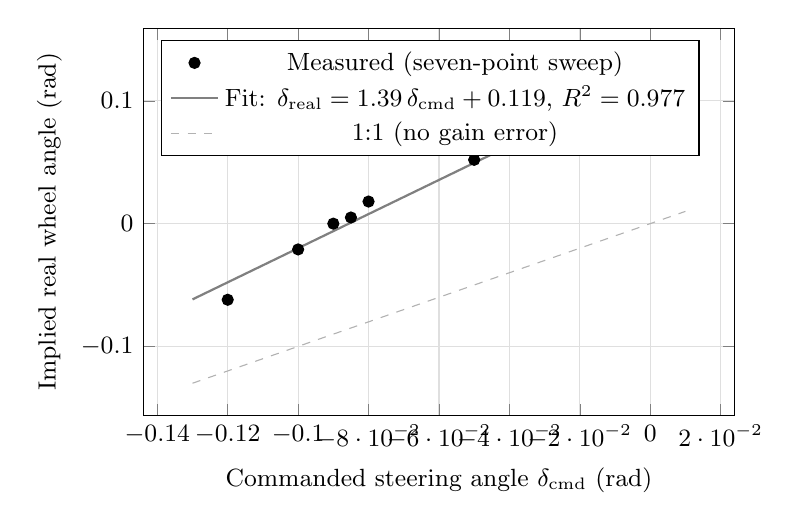
\begin{tikzpicture}
    \begin{axis}[
        width=0.75\textwidth, height=6.5cm,
        xlabel={Commanded steering angle $\delta_{\text{cmd}}$ (rad)},
        ylabel={Implied real wheel angle (rad)},
        grid=major, grid style={gray!25},
        legend pos=north west, legend style={font=\small},
        label style={font=\small}, tick label style={font=\small}
      ]
      \addplot[only marks, mark=*, mark size=2pt, color=black]
        coordinates {(0.00,0.112) (-0.05,0.052) (-0.08,0.018)
          (-0.085,0.005) (-0.09,0.000) (-0.10,-0.021) (-0.12,-0.062)};
      \addlegendentry{Measured (seven-point sweep)}
      \addplot[domain=-0.13:0.01, samples=2, thick, color=gray]
        {1.39*x + 0.119};
      \addlegendentry{Fit: $\delta_{\text{real}}=1.39\,\delta_{\text{cmd}}+0.119$, $R^2=0.977$}
      \addplot[domain=-0.13:0.01, samples=2, dashed, color=gray!60]
        {1.00*x};
      \addlegendentry{1:1 (no gain error)}
    \end{axis}
  \end{tikzpicture}
  \caption[Commanded vs.\ implied real steering angle]{Commanded versus implied real steering angle
    (Table~\ref{tab:steering-gain-sweep}), with the fitted regression
    line against the 1:1 relationship a gain-free kinematic model
    would predict. The fitted slope of 1.39 is the multiplicative gain
    error itself; the vertical offset between the two lines at
    $\delta_{\text{cmd}}=0$ separately reflects the zero-point trim
    before it was corrected.}
  \label{fig:steering-gain-fit}
\end{figure}

The relationship is clean, monotonic and shows no sign flips or
stalls. A least-squares linear fit,
$\delta_{\text{real}} = m \, \delta_{\text{cmd}} + c$, gives
$m = 1.39$, $c = \SI{0.119}{\radian}$, $R^2 = 0.977$ (the two
largest-magnitude commands sit slightly above the fitted line, a mild
hint of additional curvature at large angles not investigated
further). Two conclusions follow directly. The true zero-point
trim is $\delta_{\text{cmd}} = -0.09$, not the $-0.08$ found by the
coarser static test above, pinned by direct interpolation between
the $-0.085$ (implied $+0.005$) and $-0.09$ (implied $0.000$) rows.
Independently of the trim value entirely, the real wheel
also turns approximately 39\% \emph{further} than the kinematic model's
commanded angle implies for any non-zero command. This is a genuine
multiplicative gain error, not an offset and one that a pure trim
correction cannot fix. This gain error is a strong candidate explanation for the
original complaint that motivated the investigation. Nav2's planner
and MPPI controller both assume the kinematic model of
Section~\ref{sec:true-ackermann} maps 1:1 onto real wheel angle. A
vehicle that over-rotates by 39\% for every commanded turn would
visibly overshoot turns and cut corners tighter than planned,
exactly the symptom reported.

\paragraph{Fix and validation.} A documentation check first confirmed
that no factory steering calibration exists to consult. The Quanser
hardware manual \cite{quanser2023qcar} documents only the raw servo
command range and the physical maximum wheel angle
(Table~\ref{tab:app-safety-limits}). The HAL's own
\texttt{steeringBias} construction parameter was confirmed left at
its default of zero in \texttt{qcar\_bridge.py} -- nothing at the
firmware level was fighting or duplicating the software correction.
\texttt{STEERING\_GAIN = 1.39} (Listing~\ref{lst:trim-split}'s
\texttt{apply\_trim()}, which pre-divides the kinematic angle by this
constant before adding \texttt{STEERING\_TRIM}) was set directly from
this regression. The trim itself was then refined further, from three
repeated trials each at commanded $-0.08$, $-0.085$ and $-0.09$ (to
average out human placement and measurement noise): the zero-crossing
of the three averaged measurements gave a final
\texttt{STEERING\_TRIM = -0.087}. A dedicated validation drive commanded a real kinematic turn of
\SI{0.15}{\radian} over a \SI{1}{\meter} arc at
\SI{0.4}{\meter\per\second}, predicting \SI{28.5}{\centi\meter} of
lateral deflection. The measured deflection was \SI{27}{\centi\meter},
a residual error of $\approx$5.6\%, down from $\approx$39\% with no
gain correction at all. The fix was subsequently
confirmed in genuine closed-loop use. After re-running autonomous
Nav2 navigation on the physical vehicle post-deployment, my
direct assessment was that turning behaviour had visibly
improved. This is consistent with the gain error having been the
dominant cause of the original complaint rather than merely a
contributing factor.

As with the throttle calibration constants of
Section~\ref{sec:final-calibration}, both \texttt{STEERING\_GAIN} and
\texttt{STEERING\_TRIM} are per-unit values, expected to differ on a
different physical chassis. The empirical sweep-and-regression
\emph{method} used to find them is the transferable result, not the
specific numbers. One operational caution from this investigation is
also worth recording: testing a previously untested steering-angle
magnitude can produce more real curvature than expected. Available
clearance should be confirmed in the new command's actual curve
direction before testing it, not only in directions already validated
at smaller magnitudes.

\subsection{A Trim-Placement Bug and the ``Apply at the Actuator Boundary'' Principle}
\label{sec:trim-boundary-principle}

The first implementation of this trim contained a real bug worth
recording as a general principle for any per-unit hardware
calibration constant, not only this one. It folded the trim into the
\emph{same} steering value used both for the real servo command
\emph{and} for the odometry dead-reckoning calculation in
Section~\ref{sec:onboard-bridge-odom}. The entire purpose of
the trim is to make the real wheels read approximately zero deflection
despite a nonzero servo command. Feeding that same trimmed value into
odometry made the dead-reckoning model believe the wheels were
deflected by the trim amount, even while the vehicle was in reality
driving dead straight. A live test briefly exposed this directly: a
straight-line drive of approximately \SI{2.8}{\meter} produced a
fictitious $y \approx \SI{-1.72}{\meter}$ in the odometry output, a
spurious $\sim$\ang{30} curve that did not correspond to any real
vehicle motion.

The fix separated \texttt{compute\_steering()} (returns the
untrimmed, kinematic steering angle, used for odometry) from a new
\texttt{apply\_trim()} (computes the real servo command, called only
immediately before the HAL write), shown together in
Listing~\ref{lst:trim-split}. \texttt{target\_steering} is
\texttt{compute\_steering()}'s untrimmed return value. It is also what
Listing~\ref{lst:odometry-class}'s \texttt{odom.update()} call is
given. \texttt{apply\_trim()} is invoked only once, at the
\texttt{car.write()} call site itself.

\begin{lstlisting}[language=Python,caption={The kinematic-steering / servo-trim split (\texttt{qcar\_bridge.py}).},label={lst:trim-split}]
def compute_steering(linear_x, angular_z):
    # Returns the KINEMATIC (untrimmed) angle - used for odometry.
    # STEERING_TRIM must NOT be folded in here (see prose above).
    if abs(linear_x) < 1e-2:
        steer = 0.0
    else:
        steer = math.atan(WHEELBASE * angular_z / linear_x)
    return max(-MAX_STEER_CMD, min(MAX_STEER_CMD, steer))


def apply_trim(kinematic_steering):
    # Converts a real/kinematic steering angle into the servo command
    # that achieves it on this vehicle - call only right before
    # car.write(), never upstream of odometry or anything else that
    # treats its input as the true physical wheel angle.
    return max(-MAX_STEER_CMD,
               min(MAX_STEER_CMD,
                   kinematic_steering / STEERING_GAIN + STEERING_TRIM))
\end{lstlisting}

Re-verified with the same drive
command, the odometry then correctly read $y \approx 0$. The general
principle this illustrates is stated here explicitly, because it is
expected to generalise to any future per-unit hardware calibration
constant on this or a similar platform: a calibration constant
compensating for a specific actuator's physical imperfection should
be applied \emph{as late as possible, immediately at the actuator
boundary}. It should never be applied upstream of any computation,
such as odometry, that treats its input as an accurate, ground-truth
kinematic quantity.

\section{Clock Synchronisation and the Receipt-vs-Capture Timestamp Bug}
\label{sec:clock-offset}

The first real navigation-goal test I ran, once mapping,
localisation and the fixes above were all in place, surfaced a new
symptom: sudden AMCL localisation jumps and visible path deviation
on both straight and curved segments. The description of what was actually observed was
distinctive: LiDAR scan shape stays internally coherent, but the
entire scan rigidly shifts and appears to track the robot's motion,
``like the skeleton of the map is moving.'' That, together with an
explicit instinct that this might be a transform-related issue
rather than a tuning problem, pointed toward a \emph{timing} rather
than a spatial or gain-tuning cause -- and this proved correct.

\texttt{/scan} (port 5556) and \texttt{/odom} (port 5555) are two
independent TCP streams, each subject to its own, uncorrelated
network jitter -- this link had already been measured showing
\SIrange{87}{300}{\milli\second} of variable latency.
\texttt{qcar\_relay\_node.py} had been stamping both incoming
streams with \texttt{self.get\_clock().now()} at the moment of TCP
\emph{receipt} on the development PC, rather than at the moment of
sensor \emph{capture} on the QCar. Because the two streams' receipt
times are decorrelated, a late-arriving scan could be paired against
an odometry sample purely by receipt-time coincidence. In real
physical time, that odometry sample could already be stale by a
different, independent amount. This produces exactly the observed symptom: a
LiDAR scan that is internally self-consistent but rigidly offset
relative to the map, tracking the robot's own recent motion.

The fix required both machines' clocks to be related, not merely
each stream's own internal timing corrected. A round-trip-corrected
NTP-style offset measurement (five clustered trials of
$\text{offset} = t_{\text{remote}} - (t_1+t_2)/2$ around an SSH
\texttt{date} call) found a genuine $\sim$\SI{0.50}{\second} clock
offset between the two machines -- a naive sequential comparison
without the round-trip correction would have overstated this by also
counting SSH connection-setup time as clock skew.

\paragraph{Why the round-trip correction is needed.}
A naive measurement works like this: record a local timestamp $t_1$,
SSH into the QCar and read its clock to get $t_{\text{remote}}$, then
compute $t_{\text{remote}} - t_1$. This conflates two effects that a
single one-way measurement cannot separate. One is the genuine clock offset
between the two machines. The other is the real, nonzero time the
SSH round trip itself takes to establish a connection and execute
the remote command, which inflates the apparent gap in one direction
only.

The correction used here follows the same symmetric-delay assumption
underlying NTP itself \cite{rfc5905ntp}: record a second local timestamp $t_2$
immediately after the remote reply arrives. Treat the remote
reading as having been taken at the network's best available
estimate of the corresponding local instant -- the midpoint
$(t_1+t_2)/2$. This assumes the outbound and return legs of the
round trip take approximately equal time, which is reasonable for a
short, otherwise idle local-network SSH round trip, but would not be
for a highly asymmetric link. Averaging five such trials, rather
than trusting a single one, further reduces the influence of any one
trial's round-trip time deviating unusually from that
symmetric-delay assumption.

This offset was deliberately \emph{not} corrected via a system-level
NTP/chrony configuration, since the QCar is shared laboratory
hardware. A persistent system configuration pointing it at one
researcher's personal development machine as a time reference is
not appropriate to leave on shared infrastructure. Instead,
\texttt{qcar\_bridge.py} and \texttt{qcar\_lidar\_node.py} were
changed to stamp every message with their own local
\texttt{time.time()} at the moment of capture, added as a
\texttt{'t'} field in the JSON payload. \texttt{qcar\_relay\_node.py}
gained a \texttt{qcar\_clock\_offset} parameter and a
\texttt{qcar\_time\_to\_stamp()} helper that converts a QCar-local
capture timestamp into its development-PC-clock equivalent, applied
consistently to both the \texttt{/odom}+TF and \texttt{/scan}
publication paths. Listing~\ref{lst:clock-offset-code} shows the
conversion.

\begin{lstlisting}[language=Python,caption={Converting a QCar-local capture timestamp to the development PC's clock (\texttt{qcar\_relay\_node.py}).},label={lst:clock-offset-code}]
def qcar_time_to_stamp(qcar_time, qcar_clock_offset):
    '''Converts a QCar-clock time.time() reading into a
    builtin_interfaces/Time on this machine's clock, correcting for
    the measured offset between the two machines' independent,
    unsynchronized clocks.'''
    corrected = qcar_time - qcar_clock_offset
    sec = int(corrected)
    nanosec = int(round((corrected - sec) * 1e9))
    return Time(sec=sec, nanosec=nanosec)
\end{lstlisting}

\begin{table}[htbp]
  \centering
  \caption{Diagnostic measurements underlying the clock-offset fix.}
  \label{tab:clock-offset}
  \begin{tabular}{@{}ll@{}}
    \toprule
    Quantity & Value \\
    \midrule
    Network latency (TCP link, both ports) & \SIrange{87}{300}{\milli\second} (variable) \\
    Measured clock offset (round-trip corrected, initial session) & $\approx \SI{0.50}{\second}$ \\
    Measured clock offset (persistent-connection method, final session) & $\approx \SI{0.019}{\second}$ \\
    \texttt{qcar\_clock\_offset} launch parameter (final verified session) & \texttt{0.019} \\
    \bottomrule
  \end{tabular}
\end{table}

\paragraph{A measurement artifact found in a later session.} A
subsequent hardware session revisited this offset and found the
round-trip correction above still carries a hidden bias when each of
the five trials opens its own fresh SSH connection. Repeating the
measurement that day gave a wide, noisy spread (mean
\SI{0.93}{\second}, range \SI{0.28}{\second}--\SI{1.58}{\second})
rather than a tight, repeatable figure. Clock drift accumulates
gradually and could not explain a spread this wide within one
sitting. The actual cause was SSH's own per-connection handshake:
opening a brand-new connection for every trial front-loads that
handshake delay onto the outbound leg only, which breaks the
equal-outbound/return-delay assumption the round-trip correction
itself depends on.

Re-measuring over a single, persistent SSH connection
(\texttt{ControlMaster} multiplexing, no fresh handshake per sample)
removed this asymmetry directly. The result converged tightly to
\SI{0.019}{\second} across eleven of twelve samples, roughly two
orders of magnitude smaller than the \SI{0.50}{\second} figure
originally measured. The diagnosis and fix earlier in this section
remain correct in substance: an uncorrected receipt-timestamp
mismatch of this kind genuinely produces the display artefact
described here. Only the specific magnitude measured at the time was
inflated by the fresh-connection method's own hidden asymmetry, not
by a flaw in the receipt-vs-capture diagnosis itself.
\texttt{qcar\_clock\_offset = 0.019} is the value used in this
project's final hardware configuration.

\section{Safe Shutdown Procedure}
\label{sec:safe-shutdown}

Because two of the four processes in this bridge run directly on
physical hardware with no supervising ROS~2 lifecycle to fall back
on, this project established and documented a fixed shutdown
sequence, using \texttt{SIGINT} exclusively rather than a plain
\texttt{pkill} (per the signal-handling fix in
Section~\ref{sec:bridge-architecture}):
(1)~stop \texttt{qcar\_relay\_node.py} on the development PC;
(2)~stop the visualisation launch process group (RViz may itself
segfault on exit, a known, harmless Qt/OpenGL quirk on this system --
worth confirming it has actually exited rather than assuming);
(3)~stop \texttt{qcar\_lidar\_node.py} on the QCar;
(4)~stop \texttt{qcar\_bridge.py} on the QCar (requires \texttt{sudo}).
This project's own operational experience found it is not sufficient
to trust that the sequence \emph{was run}. On one occasion, the
motor bridge was still listening on its TCP port after I
believed it had been stopped. The documented procedure therefore
explicitly includes confirming both TCP ports (5555, 5556) are
released on the QCar (\texttt{ss -tlnp}) before considering the
vehicle idle.

\section{Summary}
\label{sec:hardware-bridge-summary}

This chapter's bridge architecture makes the physical QCar appear,
from the perspective of every ROS~2 node in the navigation stack, as
an ordinary \texttt{/cmd\_vel}-in, \texttt{/odom}/\texttt{/scan}-out
robot -- despite the underlying reality of two incompatible ROS~2
distributions connected by a bespoke TCP/JSON protocol. Getting the
data flowing across that bridge to a fidelity usable by AMCL and
Nav2, however, required four further, independently discovered
corrections (LiDAR angle convention, wheel odometry, steering trim
and inter-machine clock synchronisation) beyond simply moving bytes
across the link. Chapter~\ref{ch:calibration} continues directly from
here, addressing the one remaining discrepancy this chapter's fixes
do not touch: the relationship between a commanded velocity and the
vehicle's actual physical speed.

\chapter{System Identification and Calibration}
\label{ch:calibration}

% TODO: this is the thesis's strongest evidentiary chapter - consider
% pulling the six-point sweep and the readMode before/after table into
% actual plotted figures (velocity-vs-time traces) rather than tables
% only, if you still have the raw CSV/rosbag data from the sessions
% referenced here.

This chapter documents the longest and most consequential
investigation of the project. A real-hardware symptom emerged in
which the vehicle, commanded to travel a fixed distance and then
stop, consistently travelled substantially further before actually
coming to rest, in the worst observed case roughly three times as far.
What began as a search for a physical explanation (drivetrain
coasting) ended in the discovery of a stale-data artefact in the
vendor hardware abstraction layer described in
Section~\ref{sec:qcar-platform}. The true physical residual turned out
to be small once that artefact was removed. The chapter also
documents a control-design attempt that was tested on physical
hardware without adequate prior validation and produced a genuine,
dangerous oscillation. It is included here in full because it is as
methodologically important as the investigation's eventual successful
resolution.

\section{Problem Statement}
\label{sec:stop-distance-problem}

With the bridge of Chapter~\ref{ch:hardware-bridge} operational, a
simple closed-loop test was used throughout this investigation: drive
the vehicle at a fixed commanded speed toward a target distance,
using odometry to detect when the target is crossed and stop.
Repeated trials showed the vehicle travelling substantially further
than the commanded target before settling, with the overshoot
growing, not shrinking, across repeated sessions under otherwise
similar conditions. This was an early indication that the effect was
systematic and reproducible rather than simple measurement noise.

\section{Ruling Out Simpler Explanations}
\label{sec:ruled-out}

Several plausible causes were tested directly and eliminated before
the investigation's eventual resolution:

\begin{itemize}
  \item \textbf{AMCL/localisation.} The original suspect. Investigating
    it produced one genuine, separately valid fix. This raised AMCL's
    \texttt{recovery\_alpha\_fast}/\texttt{recovery\_alpha\_slow} from
    \texttt{0.0} to \texttt{0.1}/\texttt{0.001}, since a value of
    \texttt{0.0} allows the particle filter to freeze permanently once
    it (incorrectly) converges to zero uncertainty under real sensor
    noise. This failure mode is not exposed by a clean simulation
    environment. This fix was kept, but it does not explain the
    stop-distance symptom, which persisted after it was applied.
  \item \textbf{Command-delivery delay.} Measured directly on the
    QCar's own local clock (eliminating any network-latency
    contribution) at approximately \SI{0.2}{\second} from decision to
    applied throttle. This is normal and not large enough to explain
    metre-scale overshoot at the tested speeds.
  \item \textbf{A backlog of stale \texttt{/cmd\_vel} commands.}
    Hypothesised as queuing behind a blocking socket \texttt{send}
    call in the relay's single-threaded executor. Two increasingly
    careful fixes were built and deployed: a staleness timestamp
    check, then a full non-blocking sender-thread architecture. Both
    were tested directly on hardware. \textbf{Neither made any
    measurable difference}, ruling this out as the cause.
  \item \textbf{Logging/print buffering artefacts.} The timing of
    QCar-local debug samples during the ``coast'' period was a steady
    \SIrange{20}{35}{\milli\second} throughout, not a rapid burst
    consistent with a draining backlog -- ruled out.
\end{itemize}

\section{Active Braking as a Control-Design Attempt and a Safety Incident}
\label{sec:active-braking}

With the above ruled out, the leading hypothesis shifted to genuine
drivetrain (motor and gearbox) rotational inertia keeping the wheels
turning for a period after commanded throttle reached zero. This was
a physically plausible mechanism and one apparently consistent with
QCar-local encoder readings that showed real velocity persisting for
several seconds after a stop was commanded.

A corrective control law was implemented directly in
\texttt{qcar\_bridge.py}: a reverse-throttle brake pulse proportional
to the residual measured velocity, intended to actively cancel the
coasting motion. \textbf{This was deployed directly to physical
hardware without first being traced through by hand or tested in
simulation.} On its first test, it produced a genuine, dangerous
oscillation: the vehicle lurched forward and backward repeatedly,
reaching \SI{-0.88}{\meter\per\second} in reverse and still
accelerating. It had to be stopped manually via an SSH-issued kill
command mid-test. The root cause, in hindsight, is a textbook control
failure mode. A continuous proportional reaction to \emph{any}
nonzero residual velocity, including reverse velocity, with no
deadband and no explicit disarm condition, means every correction's
own overshoot looks to the controller like a fresh error requiring
correction. The result is an undamped hunting loop with no
mechanism to settle.

Since both attempts were reverted, no implementation of this control
law survives in the repository to quote directly. Listing~\ref{lst:active-braking-comment}
instead reproduces the comment left in its place in
\texttt{qcar\_bridge.py}, at the site the code once occupied. This is
the project's own permanent record of what was tried, why it failed
and why it must not be blindly re-attempted.

\begin{lstlisting}[language=Python,caption={Comment documenting the rejected active-braking design, left in place of the reverted code (\texttt{qcar\_bridge.py}).},label={lst:active-braking-comment}]
# Tried active braking (brief reverse-throttle pulse proportional to
# residual speed when a stop is commanded) to counter drivetrain coast -
# REJECTED, not just untuned. It's a proportional loop on velocity sign
# with no deadband and one-cycle-stale (~20ms) feedback: if the pulse
# overshoots past zero into real reverse motion, the next cycle reads a
# negative v and "corrects" with a forward push, which can itself
# overshoot - a genuine undamped hunting oscillation, not a bad gain
# value. Confirmed on hardware (twice - it was reverted once already
# before this comment, then re-tried and reproduced the same result):
# car visibly lurched forward/back repeatedly and fast, had to be
# killed manually. Do not re-add this without a real deadband/
# hysteresis or a one-shot (non-continuous) brake pulse design -
# retuning BRAKE_GAIN alone will not fix it.
\end{lstlisting}

\paragraph{A minimal model of why this design cannot be stable.}
The instability the comment above describes can be shown formally
with a deliberately simplified discrete-time model that keeps only
the mechanism responsible, not the full nonlinear vehicle dynamics.
Let $v_k$ be the residual measured velocity at control cycle $k$.
Let the brake law command a throttle proportional to that residual
with gain $K$: $u_k = -K v_k$. If the vehicle's velocity responds to
one cycle's throttle command with an effective per-cycle gain $a$
(lumping motor response, control period and vehicle mass into a
single constant and ignoring natural friction/drag for this minimal
model), the resulting closed-loop update is

\begin{equation}
  v_{k+1} = v_k + a\,u_k = v_k(1 - aK).
  \label{eq:brake-instability}
\end{equation}

This is a first-order linear recurrence. Its behaviour is
governed entirely by the magnitude of $(1 - aK)$. The residual
velocity decays toward zero only if $|1 - aK| < 1$, i.e.\
$0 < aK < 2$; it oscillates in sign every cycle if $aK > 1$.
Critically, that oscillation \emph{grows} in magnitude, without
bound, whenever $aK > 2$, since each successive $v_k$ is then
multiplied by a factor more negative than $-1$. This single
inequality is the formal statement of exactly what the source comment
describes qualitatively: a correction that overshoots past zero into
real reverse motion, prompting a next-cycle correction in the
opposite direction that itself overshoots by more. It also shows
directly why \emph{no} amount of retuning $K$ alone guarantees safety
here. $a$, the vehicle's true, real per-cycle response to a given
throttle command, was never independently measured before this
control law was deployed, so there was no way to have verified
$aK < 2$ in advance from the gain value alone.

A one-shot design avoids re-arming after the first correction, but
Equation~\ref{eq:brake-instability}'s single-step overshoot condition
does not require re-arming to manifest. If the very first correction
alone satisfies $aK > 2$, it already produces a reverse velocity
larger in magnitude than the original residual it was meant to
cancel. This is consistent with the one-shot retest reproducing the
same oscillation, rather than being protected by its disarm
condition. It is precisely the kind
of hand-traceable instability check Section~\ref{sec:methodology-overview}'s
standing rule asks for \emph{before} hardware deployment, not after.

A revised, ``one-shot'' design was implemented: braking fires exactly
once per drive-to-stop transition and permanently disarms the
instant measured velocity crosses zero, rather than re-arming from
residual drift. It \textbf{reproduced the same oscillation on
retest}. Given the repeated safety failure, this control approach was
abandoned entirely rather than iterated on further. Both modified
files were reverted to their exact pre-investigation state, verified
byte-identical to the known-good version by hash comparison. The
failure was documented directly in a source-code comment so that it
is not blindly re-attempted in a future session.

This incident is the clearest instance in this project of the general
principle stated in Section~\ref{sec:methodology-overview}. A
reactive feedback controller acting on a live sensor reading, on a
system already confirmed to have real actuator lag and inertia,
should be traced through by hand for an overshoot scenario or tested
in simulation first, before it is ever sent to physical hardware.
``The control theory seems sound'' was not, on its own,
sufficient justification here. This project treats that as a
standing rule for any future reactive control logic on this
platform, not merely a lesson learned in retrospect.

\section{Sim-versus-Real Comparison}
\label{sec:sim-vs-real}

Following a methodology suggested by my academic
supervisor, the identical closed-loop stop-distance test (drive $N$
metres at a fixed speed, stop the instant odometry crosses the
target) was reproduced in both the physical robot and the Gazebo
simulation of Chapter~\ref{ch:sim-stack}, using the same launch stack
with only the drive target switched from simulated to real hardware.

A six-point sweep across three target distances
(\SIlist{1.0;1.5;2.0}{\meter}) and three commanded speeds
(\SIlist{0.20;0.25;0.30}{\meter\per\second}) found real
hardware overshoot in the range \SIrange{0.58}{2.12}{\meter} across
two sessions roughly one hour apart. \emph{Every} tested condition
was worse in the second session, by a broadly consistent margin. This
is evidence of real, reproducible drift, plausibly battery voltage or
floor/tyre condition, rather than measurement noise.

The matched simulation sweep, over the same six conditions, showed
overshoot of only \SIrange{0.044}{0.067}{\meter} --
\SIrange{10}{30}{}$\times$ smaller and only weakly sensitive to
speed. This is in contrast to the real hardware overshoot, which
scaled roughly with the cube of speed. A dedicated, isolated
comparison at \SI{2}{\meter} / \SI{0.3}{\meter\per\second} sharpened
this further. The simulated vehicle settled at \SI{2.067}{\meter}
(an extra \SI{0.067}{\meter}), while the real vehicle settled at
\SI{3.91}{\meter} (an extra \SI{1.90}{\meter}). This is a
$\sim$28$\times$ difference for an identical software command. This
result strongly supports a real-hardware-specific controller/dynamics
cause, rather than something inherent to the stop-command approach
itself. It directly motivated the calibration work in the remainder
of this chapter.

\section{Throttle Calibration}
\label{sec:throttle-calibration}

\subsection{The Uncalibrated Gain Hypothesis}
\label{sec:throttle-gain-hypothesis}

\texttt{qcar\_bridge.py}'s mapping from \texttt{cmd\_vel}'s
\texttt{linear.x} (in \si{\meter\per\second}) to the HAL's PWM duty
cycle had, since early in the project, used a placeholder gain
(\texttt{THROTTLE\_GAIN = 1/3}), explicitly documented in its own
source comment as uncalibrated. Direct measurement from the sweep
data above confirmed this mattered. Commanding
\SI{0.3}{\meter\per\second} produced a real, QCar-local
encoder-measured cruise velocity averaging
$\approx$\SI{0.8}{\meter\per\second}, roughly $2.6$--$2.7\times$ the
commanded speed, consistent across two independent measurements.
Since coasting distance from momentum scales with the square of
velocity, this alone predicts roughly a $6.9\times$ larger coast
distance than a genuine \SI{0.3}{\meter\per\second} stop would
produce. This is a substantial fraction of the sim-vs-real gap found
above and a reminder that the sim-vs-real comparison in
Section~\ref{sec:sim-vs-real} was not, at that point, comparing truly
matched real speeds.

\subsection{A First Calibration Attempt That Discovered a Deadband, Then Reverted}
\label{sec:deadband-discovery}

A dedicated measurement tool, \texttt{check\_stop\_latency.py}, was
built to measure cruise velocity and stop latency in a single run. An
initial correction lowered \texttt{THROTTLE\_GAIN} by dividing by
the previously measured $2.67\times$ ratio. Deployed to hardware, it
immediately surfaced a second, independent, hard non-linearity. At
the old gain, a commanded \SI{0.25}{\meter\per\second} ($\sim$8\%
duty) sat completely motionless for $\approx$\SI{2.1}{\second}
before suddenly starting to move. This delay was later traced
(Section~\ref{sec:readmode-bug}) to a HAL buffering artefact rather
than a friction effect. \SIlist{0.20;0.15}{\meter\per\second}
($\sim$6.7\%/5\% duty) never moved at all across
\SIrange{8}{10}{\second} of commanding.

This second behaviour is zero motion regardless of how long the duty
is held. It is a genuine, independent physical deadband property of
the vehicle, not a linear gain error. It interacts badly with a
naive linear-gain correction: the lowered gain restored accurate
cruise-speed tracking at higher commanded speeds, but pushed the
duty cycle for normal teleoperation speeds below the deadband
threshold entirely, making the vehicle stop responding to real
driving commands. The gain correction was reverted
the same day to restore usable teleoperation.

\paragraph{This is a different friction phenomenon from Section~\ref{sec:friction-theory}'s -- and, in part, not friction at all.}
It is worth being precise about which effects are actually responsible
here, since this thesis initially conflated two genuinely distinct
physical phenomena with a third, unrelated software artefact, all
under similar friction-flavoured language. Section~\ref{sec:friction-theory}'s
Coulomb tyre-ground friction (the simulation's \texttt{mu1}/\texttt{mu2})
governs whether a spinning wheel's rotation converts into forward
chassis thrust at all and is essentially instantaneous. It has no
notion of a wheel being ``stuck'' and is unrelated to everything
below. The deadband characterised here is a different phenomenon
internal to the real drivetrain itself (motor brushes, gearbox mesh,
bearing seats): \emph{static} friction (often called stiction) resists
the onset of relative motion between two surfaces up to some breakaway
force threshold, while \emph{kinetic} friction, which applies once
motion has actually begun, is often measurably lower than that static
threshold for the same surface pair. A commanded duty cycle below the
static threshold produces zero motion no matter how long it is held,
since the applied torque never exceeds the force needed to break
static friction in the first place. This zero/non-zero threshold is
genuinely real and remains present after every fix in this chapter
(Section~\ref{sec:readmode-validation}).

What is \emph{not} a friction effect, despite initially being
described as one here, is the multi-second delay observed
\emph{before} that breakaway. Section~\ref{sec:readmode-bug} shows
this $\approx$\SI{2}{\second} figure is fixed regardless of duty,
speed, or how much torque is applied, something a genuine
breakaway-force process would not produce. It traces the delay
instead to a buffered sensor read in the vendor HAL.

Once duty is raised past the real static threshold, the \emph{lower}
kinetic friction then applies to an already-moving system, so the
same duty cycle that only barely broke static friction can
accelerate substantially further than expected once moving. This
asymmetry, unlike the delay, is a genuine, still-valid physical
effect. It is the stick-slip signature Section~\ref{sec:final-calibration}
identifies directly in the duty-sweep data. Table~\ref{tab:duty-sweep}'s
\texttt{0.085} row \emph{runs away} to a sustained higher
cruise speed rather than settling, a continuing behavioural
difference rather than a one-off timing offset.

This reframes the calibration problem: gain and deadband are not
independent. Any solution must jointly (a) track commanded speed
accurately at normal operating speeds and (b) keep every one of
those same commands above the static-friction threshold. A single
linear multiplier applied to the whole range cannot do both: scaling
the gain down to fix (a) simultaneously worsens (b), for exactly the
commands that were already only barely clearing the threshold.

\subsection{Final Calibration via an Empirical Duty Sweep}
\label{sec:final-calibration}

Given that finding, the calibration approach was reframed entirely:
rather than extrapolating a linear gain from one or two data points,
\texttt{THROTTLE\_GAIN} was forced to zero and a dedicated,
lighter-weight tool (\texttt{drive\_and\_log.py}) was used to sweep
fixed PWM duty values directly, with the vehicle on the ground under
real load throughout. Table~\ref{tab:duty-sweep} summarises the
resulting duty-response curve.

\begin{table}[htbp]
  \centering
  \caption{Fixed-duty sweep results (QCar on the ground, real load).}
  \label{tab:duty-sweep}
  \begin{tabular}{@{}p{2cm}p{12.5cm}@{}}
    \toprule
    Duty & Observed behaviour \\
    \midrule
    0.050 & No motion at all (confirmed twice, up to \SI{27.5}{\second} of commanding) \\
    0.060--0.061 & Reliable breakaway after an initial $\approx$\SIrange{2.0}{2.1}{\second} start-up delay (later traced to a HAL buffering artefact, Section~\ref{sec:readmode-bug}, not friction); settles to a stable, non-runaway cruise of $\approx$\SIrange{0.24}{0.33}{\meter\per\second} \\
    0.065 & $\approx$\SI{0.39}{\meter\per\second} \\
    0.085 & \textbf{Runs away} to $\approx$\SIrange{0.85}{0.9}{\meter\per\second} -- a stick-slip signature (static friction exceeds kinetic friction, so once moving, the same duty produces far more net accelerating force), confirmed by watching the full velocity trace climb continuously rather than plateau \\
    \bottomrule
  \end{tabular}
\end{table}

A caution surfaced during this sweep and worth recording explicitly:
the motion/no-motion threshold near duty $\approx 0.06$ is genuinely
noisy, not a hard deterministic cut-off. A re-test with duty
adjusted by only $+0.0013$ (\texttt{0.0533} vs.\ \texttt{0.052})
flipped a command from ``27\,s of zero motion'' to reliably covering
the full target distance. This floor appears to drift somewhat both
within and across sessions (plausibly floor contact, resting wheel
position, temperature, or battery voltage). No single threshold
measurement from this sweep should be treated as an exact, permanent
constant.

The deployed calibration combines a deadband floor with a linear gain
above it, fit from the duty=0.061/\SI{0.33}{\meter\per\second} and
duty=0.065/\SI{0.39}{\meter\per\second} points and validated
separately:

\begin{align}
  \text{duty} &= \text{THROTTLE\_DEADBAND} + \text{THROTTLE\_GAIN} \cdot |v_{\text{cmd}}|, \notag\\
  \text{THROTTLE\_DEADBAND} &= 0.04,\quad \text{THROTTLE\_GAIN} = 0.0667.
  \label{eq:throttle-calibration}
\end{align}

Listing~\ref{lst:throttle-formula} shows Equation~\ref{eq:throttle-calibration}
as implemented in \texttt{qcar\_bridge.py}'s control loop, together
with the rate limiter that caps how fast \texttt{current\_throttle}
(the value actually written to the HAL) may change per cycle. This is
a separate safeguard from the deadband/gain calibration itself,
present throughout this chapter's testing to keep duty-cycle steps
within the documented \SI{100}{\percent\per\second} hardware limit
(Appendix~\ref{app:safety-limits}).

\begin{lstlisting}[language=Python,caption={Duty-cycle command computation and rate limiting (\texttt{qcar\_bridge.py}).},label={lst:throttle-formula}]
if abs(target_linear) < 1e-3:
    desired_throttle = 0.0
else:
    desired_throttle = math.copysign(
        THROTTLE_DEADBAND + THROTTLE_GAIN * abs(target_linear), target_linear)
desired_throttle = max(-THROTTLE_LIMIT, min(THROTTLE_LIMIT, desired_throttle))
max_step = THROTTLE_RATE_LIMIT * dt
delta = max(-max_step, min(max_step, desired_throttle - current_throttle))
current_throttle += delta
\end{lstlisting}

Table~\ref{tab:calibration-validation} presents the resulting
end-to-end validation across four commanded speeds, each from a
dedicated \SI{2}{\meter} drive-and-stop test with cruise velocity
measured directly from \texttt{/odom}.

\begin{table}[htbp]
  \centering
  \caption{Throttle calibration validation (Equation~\ref{eq:throttle-calibration}).}
  \label{tab:calibration-validation}
  \begin{tabular}{@{}lccc@{}}
    \toprule
    Commanded speed & Measured cruise speed & Ratio & Note \\
    \midrule
    \SI{0.2}{\meter\per\second} & unreliable ($\approx$0.24 or no motion) & -- & At the deadband edge \\
    \SI{0.3}{\meter\per\second} & \SI{0.31}{\meter\per\second} & 1.05 & \\
    \SI{0.4}{\meter\per\second} & \SI{0.42}{\meter\per\second} & 1.05 & \\
    \SI{0.5}{\meter\per\second} & \SI{0.50}{\meter\per\second} & 1.00 & \\
    \bottomrule
  \end{tabular}
\end{table}

This is a substantial improvement over the original uncalibrated
gain's $2.6$--$2.7\times$ overshoot: commanded speeds of
\SIrange{0.3}{0.5}{\meter\per\second} now track within
$\approx$5\%. Below $\approx$\SIrange{0.25}{0.3}{\meter\per\second},
open-loop duty control against real floor/battery/temperature-dependent
friction is inherently unreliable. This is treated as a hard
physical limit of the open-loop approach at the tested operating
conditions, not a remaining tuning gap. Reliable
sub-\SI{0.25}{\meter\per\second} creep would require closed-loop
velocity feedback from the encoder, rather than a fixed duty
mapping.

\subsection{A Stray-Process False Positive}
\label{sec:stray-process}

While iterating on this calibration, a separate, purely diagnostic
false alarm is worth recording as a general debugging caution. A
prior \texttt{check\_stop\_latency.py} test process, left running in
the background rather than exiting automatically once its measurement
completed, continued publishing \texttt{linear.x=0.0} on
\texttt{/cmd\_vel} at 20\,Hz, silently racing against a separately
launched teleoperation node publishing on the same topic. The
resulting symptom was the vehicle briefly registering a throttle
command and then immediately reverting to zero within one control
cycle. It looked exactly like a gain, deadband, or logic bug and was
initially investigated as one. ROS~2 does not warn about multiple
publishers on the same topic; it simply interleaves messages, with
whichever publisher's message arrives last in a given control cycle
taking effect. The actual fix was operational, not code: kill the
stray process. This project subsequently adopted two standing
practices as a result: checking \texttt{pgrep -af} for
topic-related script names (or \texttt{ros2 topic info /cmd\_vel
--verbose} for publisher count) before deep-diving into a
control-logic theory whenever real behaviour contradicts an issued
command; and designing one-shot diagnostic nodes to exit
automatically once their measurement is complete, rather than
spinning indefinitely.

\section{The Hardware Abstraction-Layer Buffering Defect}
\label{sec:readmode-bug}

The original stop-distance symptom this chapter opened with is a
multi-second coast after a stop command, with substantial extra
distance. Even after the throttle calibration of
Section~\ref{sec:final-calibration} made commanded and real cruise
speed match closely, that symptom was still present, apparently
unaffected by the gain fix. This section documents how that residual
was ultimately traced to a defect in the vendor hardware abstraction
layer itself, not the vehicle's physical dynamics at all. This is
the project's single most significant finding, both for its
magnitude and for the methodological lesson in how long an incorrect
physical explanation can survive against evidence that, in
hindsight, directly contradicted it.

\subsection{An Initial, Incomplete Diagnosis}
\label{sec:coast-shape-analysis}

A closer look at the raw coast-phase velocity trace from one of the
calibration validation runs (\SI{0.5}{\meter\per\second}) showed the
coast was \emph{not} a smooth decay. Velocity remained essentially
flat, if anything slightly \emph{elevated} relative to the preceding
cruise average, for the first $\approx$\SI{2.0}{\second} after
``stop'' was commanded. It then crashed sharply to zero in the final
\SIrange{0.3}{0.4}{\second}. This flat-plateau-then-cliff shape
is inconsistent with passive drivetrain momentum/friction coasting
(which predicts continuous, gradual decay starting immediately once
power is cut) and instead resembles the real motor continuing to be
\emph{actively driven} for roughly two seconds after the stop command
was issued. A review of the Quanser HAL documentation
\cite{quanser2023qcar} found no
mention of any drive-motor ramp, filter, or time constant that would
explain a two-second lag of this kind -- only a separate, documented
\SI{0.16}{\second} steering-servo time constant, unrelated to the
drive motor. This shifted the leading hypothesis toward a
command-delivery lag in the project's own bridge software, rather
than physical coasting. This was a genuine change of theory,
captured here because it turned out to still be one step short of
the actual cause. A
diagnostic instrumentation pass (logging commanded velocity, the
bridge's own internally-ramped throttle value and real encoder
velocity together, all on the QCar's local clock to eliminate network
timing) was begun but interrupted by the test vehicle's battery
running out mid-session and resumed in a later session on a charged
battery.

\subsection{Disproving Two Hypotheses and the Argument That Found the Real Cause}
\label{sec:readmode-discovery}

The resumed diagnostic trace showed the bridge's own internal
throttle value reaching exactly zero within \SI{52}{\milli\second} of
the stop command, while the encoder-reported velocity stayed elevated
for roughly two more seconds. This correctly ruled out the project's
own throttle-ramping logic as the cause. As understood in hindsight,
though, it did \emph{not} actually rule out a measurement or
reporting defect in the encoder-velocity reading itself, since the
two values are produced through entirely separate code paths. This
distinction was missed on the first pass through the data.

At this point the person operating the vehicle directly and
repeatedly disputed the emerging conclusion. Teleoperating the QCar
from a genuine standstill, the vehicle visibly starts and stops moving
\emph{instantly} in response to a command. This flatly contradicts the
$\approx$2-second delay the automated test script was measuring. Two
further hypotheses were tested and disproven with direct hardware data
before the actual cause was found:

\begin{itemize}
  \item \textbf{Duty-magnitude dependence} (a higher commanded speed
    produces more torque and a faster breakaway): tested at
    \SI{0.7}{\meter\per\second} (duty 0.087, well above the normally
    tested \SIrange{0.052}{0.075} range) -- the start-up delay was
    still \SI{2.092}{\second}, statistically identical to the
    low-speed tests. Disproven.
  \item \textbf{``\texttt{v} is a stale reading, not real motion.''}
    Disproven by the structure of the \texttt{Odometry} class's own
    update code. The reported velocity \texttt{v} and the accumulated
    position \texttt{x} are computed from the exact same
    \texttt{distance} variable within the same loop iteration. If
    \texttt{v} were falsely indicating motion, the accumulated position
    would have to freeze at the same instant. It demonstrably did
    not: distance kept growing smoothly and matched the vehicle's real,
    physically measured settled position.
\end{itemize}

The argument that ultimately identified the true cause was not a
further measurement, but a piece of physical reasoning I raised
directly: \emph{an encoder is a real-time
sensor -- it cannot have a built-in two-second lag by itself.} This
was correct. It redirected the investigation to a question the
prior analysis had not actually asked: not whether the
\texttt{Odometry} class was internally self-consistent (it was), but
whether the value it was consuming as its own input, the raw
\texttt{car.motorEncoder[0]} read, was itself stale before the
\texttt{Odometry} class ever saw it. This prompted reading the vendor
HAL's own Python source directly, rather than continuing to reason
about it indirectly from documentation or from the \texttt{Odometry}
class's own behaviour.

\subsection{The Root Cause, a Ring-Buffer I/O Mode}
\label{sec:readmode-rootcause}

The root cause, found in the vendor HAL source
(\texttt{pal/products/qcar.py}) on the QCar itself, is exactly the
\texttt{readMode} distinction introduced in
Section~\ref{sec:qcar-platform}. \texttt{qcar\_bridge.py} constructed
its \texttt{QCar} object with \texttt{readMode=1} (task-based I/O).
This starts a background acquisition task \emph{at object
construction time}, before the bridge's listening TCP socket has even
opened. It fills a ring buffer of \texttt{frequency}$\times 2$
samples (at this project's \SI{50}{\hertz} read rate, exactly 100
samples, i.e.\ \SI{2.0}{\second}) with overwrite-on-overflow
behaviour. Each call to \texttt{car.read()} dequeues one buffered
sample. Because \texttt{car.read()} is not actually called until a
relay client connects, which can take many seconds after the bridge
process starts, the buffer fills and cycles during that idle gap.
Once reads begin at a consumption rate matching the production rate
exactly, the read stream is permanently stuck approximately 100
samples (\SI{2.0}{\second}) behind real time, because the backlog
never has an opportunity to drain.

\paragraph{Formalising the lag: why it is exactly the buffer depth, forever.}
Figure~\ref{fig:ringbuffer-lag} illustrates the mechanism derived
below. Let the background task write into the ring buffer at a fixed
production index $p$, incrementing by one every $1/f$ seconds
($f = \SI{50}{\hertz}$ here). Let \texttt{car.read()} calls
advance a separate consumption index $c$, each call returning the
sample at position $c \bmod B$ (buffer capacity $B = 100$) and then
incrementing $c$. Production begins at object construction, $t = 0$;
consumption begins only once a relay client connects, at
$t = T_{\text{idle}}$. During $[0, T_{\text{idle}}]$, $p$ advances
alone (production with no consumption at all), so by the time
consumption starts, $p = f \cdot T_{\text{idle}}$ while $c = 0$.
This is a gap of $f \cdot T_{\text{idle}}$ samples between them. If
$T_{\text{idle}} > B/f$ (true here, since a relay connecting takes
several seconds while $B/f = \SI{2.0}{\second}$), the overwrite-on-overflow
buffer has already wrapped around at least once by
$T_{\text{idle}}$. This means the oldest sample still available to
read is not the very first one produced, but the one produced exactly
$B$ samples before $p$'s current value. The very first
\texttt{car.read()} call, at $t = T_{\text{idle}}$, therefore
necessarily returns a sample captured at $t = T_{\text{idle}} - B/f$, a lag of
exactly $B/f = \SI{2.0}{\second}$, regardless of how much larger than
$B/f$ the idle gap $T_{\text{idle}}$ itself was. Production and
consumption both advance at the identical rate $f$ from that point
onward (one \texttt{car.read()} per control-loop cycle, matching the
background task's own sampling rate). Because of that, the gap
between $p$ and $c$ (and therefore the lag between ``now'' and
whatever sample is being read) stays fixed at exactly $B$ samples
indefinitely. Neither index ever gains on the other, so the backlog
that accumulated during the idle gap is carried forward forever
rather than draining over time. This is precisely why the lag proved
so exactly reproducible (always $B/f = \SI{2.0}{\second}$, never more
and never less, regardless of how long the QCar sat idle before a
relay connected) and why it never improved on its own the longer the
system ran.

\begin{figure}[htbp]
  \centering
  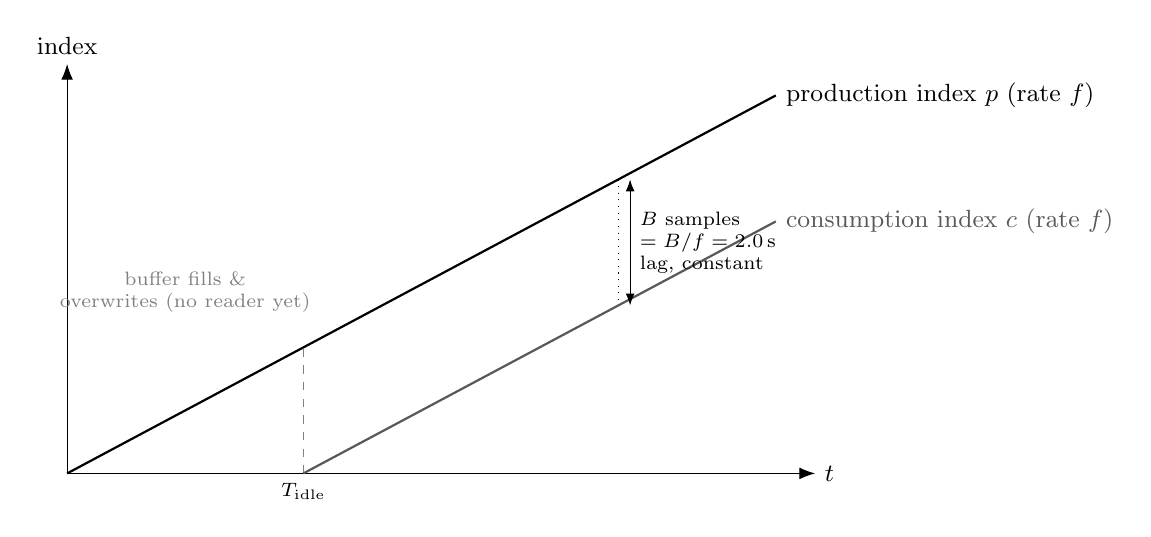
\begin{tikzpicture}[scale=1.0]
    % Axes
    \draw[-{Latex[length=2mm]}] (0,0) -- (9.5,0) node[right, font=\small] {$t$};
    \draw[-{Latex[length=2mm]}] (0,0) -- (0,5.2) node[above, font=\small] {index};

    % Production line p(t): starts at t=0, slope f, runs the whole width
    \draw[thick] (0,0) -- (9,4.8) node[right, font=\small] {production index $p$ (rate $f$)};

    % Idle gap marker on the t-axis
    \draw[dashed, gray] (3,0) -- (3,1.6);
    \node[below, font=\scriptsize] at (3,0) {$T_{\text{idle}}$};

    % Consumption line c(t): starts at t=T_idle (x=3), same slope, offset down by B (i.e. lag of B/f in time)
    \draw[thick, color=gray!70!black] (3,0) -- (9,3.2) node[right, font=\small, color=gray!70!black] {consumption index $c$ (rate $f$)};

    % Vertical gap annotation at t=7
    \draw[dotted] (7,{4.8*7/9}) -- (7,{3.2*(7-3)/6});
    \draw[{Latex[length=1.5mm]}-{Latex[length=1.5mm]}] (7.15,{4.8*7/9}) -- (7.15,{3.2*(7-3)/6})
      node[midway, right, font=\scriptsize, align=left] {$B$ samples\\$=B/f=\SI{2.0}{\second}$\\lag, constant};

    % Mark buffer wrap point
    \node[font=\scriptsize, gray, align=center] at (1.5,2.3) {buffer fills \&\\overwrites (no reader yet)};
  \end{tikzpicture}
  \caption[Ring-buffer production/consumption lag over time]{Production index $p$ (background acquisition task, running
    from $t=0$) versus consumption index $c$ (\texttt{car.read()}
    calls, starting only once a relay connects at $t=T_{\text{idle}}$).
    Both advance at the same rate $f$ once consumption begins, so the
    gap present at $t=T_{\text{idle}}$, exactly the buffer depth $B$
    once the buffer has wrapped, never closes.}
  \label{fig:ringbuffer-lag}
\end{figure}

This single mechanism explains every property of the symptom observed
across this entire chapter: the near-exact \SI{2.0}{\second} to
\SI{2.1}{\second} figure (matching the buffer's mathematically exact
2.0\,s capacity), its remarkable stability across sessions, vehicle
speeds and physical conditions (a fixed buffer depth is indifferent
to any of these) and its symmetric appearance on both the start side
(the start-up delay of Section~\ref{sec:deadband-discovery}) and the
stop side (the ``coast''), since both are read through the same
buffered path.

\textbf{Fix:} \texttt{qcar\_bridge.py} now constructs the \texttt{QCar}
object as shown in Listing~\ref{lst:readmode-fix} -- immediate I/O,
reading current hardware state directly with no background task or
buffer involved at all.

\begin{lstlisting}[language=Python,caption={The one-line HAL construction change that fixed the buffering defect (\texttt{qcar\_bridge.py}).},label={lst:readmode-fix}]
# readMode=0 (immediate I/O) - was 1 (task-based I/O), which runs a
# background acquisition task into a 100-sample ring buffer
# (frequency*2) from the moment this object is constructed,
# independent of when car.read() actually starts being called. Since
# this object is created before the listening socket even opens, and
# car.read() isn't called until a relay connects, the buffer fills and
# starts overwriting during that gap - once reads begin at the matched
# 50Hz rate, they get permanently stuck ~100 samples (~2.0s) behind
# real-time, since the backlog never drains. Immediate I/O reads
# current hardware state directly, no task/buffer involved.
car = QCar(readMode=0, frequency=READ_RATE)
\end{lstlisting}

\subsection{Validation}
\label{sec:readmode-validation}

The full calibration test suite from Section~\ref{sec:final-calibration}
was re-run in its entirety on a freshly charged battery, with the
duty formula (Equation~\ref{eq:throttle-calibration}) unchanged, to
isolate the effect of this single fix. Table~\ref{tab:readmode-fix}
presents the results.

\begin{table}[htbp]
  \centering
  \caption{Effect of the \texttt{readMode=0} fix on start-up delay, extra distance and stop latency.}
  \label{tab:readmode-fix}
  \begin{tabular}{@{}lccc@{}}
    \toprule
    Test & Start-up delay & Extra distance & Stop latency \\
    & (before $\to$ after) & (before $\to$ after) & (before $\to$ after) \\
    \midrule
    \SI{2}{\meter} @ \SI{0.3}{\meter\per\second} & \SIrange{2.09}{0.117}{\second} & \SIrange{0.520}{0.114}{\meter} & \SIrange{2.37}{0.598}{\second} \\
    \SI{2}{\meter} @ \SI{0.4}{\meter\per\second} & \SIrange{2.14}{0.001}{\second} & \SIrange{0.790}{0.114}{\meter} & \SIrange{2.40}{0.501}{\second} \\
    \SI{2}{\meter} @ \SI{0.5}{\meter\per\second} & \SIrange{2.14}{0.116}{\second} & \SIrange{0.923}{0.154}{\meter} & \SIrange{2.55}{0.550}{\second} \\
    \SI{1}{\meter} @ \SI{0.3}{\meter\per\second} & \SIrange{2.14}{0.120}{\second} & \SIrange{0.641}{0.118}{\meter} & \SIrange{2.44}{0.572}{\second} \\
    \SI{3}{\meter} @ \SI{0.3}{\meter\per\second} & \SIrange{2.08}{0.088}{\second} & \SIrange{0.583}{0.104}{\meter} & \SIrange{2.35}{0.509}{\second} \\
    \bottomrule
  \end{tabular}
\end{table}

Start-up delay collapses to \SIrange{0.001}{0.12}{\second} -- an
essentially instantaneous breakaway response, matching direct
observation of the vehicle. Extra distance becomes small and roughly
constant, $\approx$\SIrange{0.10}{0.15}{\meter}, regardless of speed
or target distance, rather than scaling with cruise speed as
previously found. This confirms that the earlier ``extra distance
scales with speed'' relationship was itself an artefact of a
fixed-\emph{duration} buffering delay applied to different real
velocities, not a genuine vehicle property.

Both the extra-distance and stop-latency figures in
Table~\ref{tab:readmode-fix} are encoder-derived, from wheel rotation
counts via \texttt{/odom}, as Section~\ref{sec:readmode-discovery}
establishes. At each of the tested distances, the encoder-reported
travel was independently cross-checked against tape-measured floor
markings and manual stopwatch timing of the commanded-stop-to-physical-stop
interval. The two agreed. This confirms the encoder as an
accurate proxy for real physical distance and timing, rather than a
further source of measurement error.

The small residual that remains after this fix is real and is fully
accounted for by ordinary physics, rather than being a further open
mystery. Dividing extra distance by stop latency, an implied average
coast velocity, yields \SIrange{54}{61}{\percent} of cruise velocity
in four of the five tests. This is consistent with an ordinary,
roughly linear velocity decay to zero over the stop-latency window (a
perfectly linear decay predicts exactly 50\%). The one outlier
(\SI{2}{\meter} @ \SI{0.3}{\meter\per\second}, 108\%) is attributable
to a data-analysis artefact (the ``cruise average'' window for that
specific test likely had not reached a true steady state, now that
the run has much less runway once start-up delay is near-instant)
rather than a physical inconsistency.

\SI{0.2}{\meter\per\second} remains genuinely unreliable even after
this fix, sometimes failing to move the vehicle at all. This is the
real, independent static-friction deadband characterised in
Section~\ref{sec:deadband-discovery} and is unrelated to the
buffering defect resolved here.

\section{Summary}
\label{sec:calibration-summary}

This chapter's investigation began with a symptom: travelling
roughly three times the commanded stop distance. This symptom had at
least three superficially plausible explanations: localisation error,
command-delivery delay and physical drivetrain coasting. It ended
by identifying two genuinely independent, compounding causes. One
was an uncalibrated, non-linear throttle-to-speed mapping
(Section~\ref{sec:throttle-calibration}). The other was a
fixed-duration sensor-read buffering artefact in the vendor hardware
abstraction layer (Section~\ref{sec:readmode-bug}) that had, for a
period of this project, been reasonably but incorrectly attributed
to genuine vehicle physics.

Neither cause was found by reasoning from documentation or first
principles alone. Both required direct, targeted measurement on the
physical robot. The second was found only after I raised a direct
physical argument that prompted reading the vendor's
own source code, rather than continuing to trust an internally
self-consistent, but incompletely verified, software abstraction.
Chapter~\ref{ch:nav-integration} builds on this
chapter's calibrated, buffering-free bridge to bring up and validate
full closed-loop Nav2 navigation on the physical vehicle.

\chapter{Navigation Integration and Validation}
\label{ch:nav-integration}

% TODO: this chapter's final section (6.5) reports a QUALITATIVE
% end-to-end result ("working almost perfectly") without a fresh
% quantitative monitor_goal_timing.py re-run post-readMode-fix. If you
% can still get lab time on the QCar, re-running that tool and
% dropping the numbers into Table 6.2 (currently a TODO) would close
% the one open loop in this thesis's results and make Ch. 7 stronger.

This chapter describes bringing the full Nav2 navigation stack up
against the physical QCar, building on the bridge of
Chapter~\ref{ch:hardware-bridge} and the calibration of
Chapter~\ref{ch:calibration}. Section~\ref{sec:nav2-porting} covers
porting the simulation-tuned Nav2 configuration to hardware.
Section~\ref{sec:mppi-critic} describes a custom MPPI critic plugin
developed for this vehicle. Section~\ref{sec:phased-integration}
reports the phased bring-up used to de-risk the integration.
Section~\ref{sec:display-lag} presents a detailed timing
investigation into an apparent localisation-display artefact, and
Section~\ref{sec:final-validation} reports the resulting end-to-end
validation.

\section{Porting the Nav2 Configuration to Hardware}
\label{sec:nav2-porting}

The Nav2 parameter set developed and tuned in simulation
(Chapter~\ref{ch:sim-stack}) required a small, mechanical set of
changes to run against physical hardware rather than Gazebo: every
occurrence of \texttt{use\_sim\_time} (13 in total, across the
costmap, planner, controller, and AMCL parameter blocks) was switched
from \texttt{true} to \texttt{false}, since the physical robot has no
simulation clock to synchronise against. Both mapping and navigation
launch files were given a real-hardware branch, gated on
\texttt{launch\_sim}, alongside the existing Gazebo branch, with
real hardware as the default and simulation opt-in
(\texttt{launch\_sim:=true}) -- a deliberate inversion of which mode
is the default, made once hardware became the project's active
development target, while keeping the simulation path fully intact
for future regression testing rather than removing it.

The AMCL \texttt{recovery\_alpha\_fast}/\texttt{recovery\_alpha\_slow}
fix from Section~\ref{sec:ruled-out} was carried forward
proactively into the hardware configuration at this point, rather
than left to be independently rediscovered against hardware, since
the underlying cause -- Section~\ref{sec:amcl-math}'s augmented-MCL
random-particle-injection mechanism being permanently disabled at
$\alpha_{\text{slow}} = \alpha_{\text{fast}} = 0$, leaving the filter
with no way to recover from an overconfident convergence once real
sensor noise (which a clean simulation rarely exercises) triggers one
-- is a property of AMCL's own resampling algorithm, not specific to
any one deployment target.

\section{Custom MPPI Critic: \texttt{EarlyCommitCritic}}
\label{sec:mppi-critic}

Early navigation testing showed a specific weakness in the stock MPPI
critic set (Section~\ref{sec:nav2}) for this vehicle: the standard
path-following critics evaluate a sampled trajectory's alignment and
progress against the path as a whole, which can leave the controller
driving further into an approaching curve before it begins reacting
to it, rather than beginning the turn as early as physically sensible
-- a behaviour more forgiving for a differential-drive robot's tight
turning radius than for an Ackermann-steered vehicle with the
finite minimum turning radius of Table~\ref{tab:qcar-geometry}.

A custom MPPI critic plugin, \texttt{EarlyCommitCritic}, was
developed and built into the navigation package to address this: it
scores only the first \texttt{early\_time\_steps} of each sampled
trajectory rollout against the bearing to a near-term path point,
with no distance or angle gating, so that MPPI is pushed to begin
turning toward the path immediately rather than waiting until deeper
into the curve. It is gated by an \texttt{active\_path\_points}
parameter so that it stops influencing the controller once the
vehicle has made genuine progress along the route, avoiding
interference with the stock critics' normal path-tracking behaviour
during straight segments. A later direction-awareness refinement
extended the critic to handle reversing and K-turn path segments
correctly, where a naive ``always turn toward the next point''
bearing calculation would otherwise fight the vehicle's intended
direction of travel.

Building this plugin required matching \texttt{xtensor}/\texttt{xsimd}
compile definitions exactly against Nav2's own MPPI controller build
-- a mismatch here does not produce a compile-time error, but a
silent ABI incompatibility that crashes the navigation container on
the first control cycle that touches vectorised critic math, making
it a notably unforgiving class of build-configuration bug to diagnose
from its symptom alone.

Listing~\ref{lst:early-commit-critic} shows the critic's
\texttt{score()} method in full. It computes the bearing from each
sampled trajectory's own starting position to a near-term path target
(\texttt{offset\_from\_furthest} points ahead of the furthest point
the robot has already reached), then, for only the first
\texttt{early\_time\_steps} of that trajectory, accumulates the
angular distance between the trajectory's actual yaw and that
bearing -- scoring every sampled rollout independently, not just the
robot's single current pose. The early return on
\texttt{active\_path\_points} is what confines this to the start of a
path, and the \texttt{forward\_preference\_}-gated minimum of the
forward- and reverse-bearing angular distances is the
direction-awareness refinement mentioned above, letting a trajectory
be scored against whichever of the bearing or its reverse it is
actually closer to, rather than penalising a legitimate reversing
manoeuvre.

\begin{lstlisting}[language=C++,caption={\texttt{EarlyCommitCritic::score()} (\texttt{src/critics/early\_commit\_critic.cpp}).},label={lst:early-commit-critic}]
void EarlyCommitCritic::score(CriticData & data)
{
  if (!enabled_ || data.path.x.shape(0) < 2) { return; }
  utils::setPathFurthestPointIfNotSet(data);

  // Only relevant at the start of a path - once the robot has made
  // real progress, let the normal path/goal critics take over.
  if (*data.furthest_reached_path_point >= active_path_points_) { return; }

  const size_t path_size = data.path.x.shape(0) - 1;
  const size_t offseted_idx = std::min(
    *data.furthest_reached_path_point + offset_from_furthest_, path_size);
  const float target_x = data.path.x(offseted_idx);
  const float target_y = data.path.y(offseted_idx);

  const size_t time_steps = data.trajectories.x.shape(1);
  const size_t early_steps = std::min(early_time_steps_, time_steps);
  if (early_steps == 0) { return; }

  const xt::xtensor<float, 1> x0 = xt::view(data.trajectories.x, xt::all(), 0);
  const xt::xtensor<float, 1> y0 = xt::view(data.trajectories.y, xt::all(), 0);
  const xt::xtensor<float, 1> bearing = xt::atan2(target_y - y0, target_x - x0);
  const xt::xtensor<float, 1> reverse_bearing = bearing + static_cast<float>(M_PI);

  xt::xtensor<float, 1> sum_diff = xt::zeros<float>({data.trajectories.x.shape(0)});
  for (size_t t = 0; t < early_steps; ++t) {
    const xt::xtensor<float, 1> yaw_t = xt::view(data.trajectories.yaws, xt::all(), t);
    const xt::xtensor<float, 1> fwd_diff =
      xt::abs(utils::shortest_angular_distance(yaw_t, bearing));
    if (forward_preference_) {
      sum_diff += fwd_diff;
    } else {
      const xt::xtensor<float, 1> rev_diff =
        xt::abs(utils::shortest_angular_distance(yaw_t, reverse_bearing));
      sum_diff += xt::minimum(fwd_diff, rev_diff);
    }
  }
  const xt::xtensor<float, 1> cost = sum_diff / static_cast<float>(early_steps);
  data.costs += xt::pow(cost * weight_, power_);
}
\end{lstlisting}

\paragraph{How this cost actually changes which trajectory wins.}
Connecting this directly to Section~\ref{sec:mppi-math}'s softmax
weighting (Equation~\ref{eq:mppi-weight}): \texttt{data.costs} is the
same per-trajectory accumulator every enabled critic adds into, so
this critic's contribution
$\left(\overline{\Delta\theta} \cdot \texttt{weight\_}\right)^{\texttt{power\_}}$
(the early-steps-averaged angular difference $\overline{\Delta\theta}$
from the listing's \texttt{cost} variable, scaled and exponentiated by
its own configured weight and power) is simply summed alongside the
stock critics' own contributions into $S(\tau^{(k)})$ before
Equation~\ref{eq:mppi-weight}'s exponential weighting is applied.
Concretely: of two sampled trajectories approaching the same curve,
one that begins turning toward the near-term path point immediately
accrues a small $\overline{\Delta\theta}$ over its first
\texttt{early\_time\_steps}, while one that continues driving straight
before reacting accrues a much larger one -- inflating that second
trajectory's total cost $S(\tau^{(k)})$, which Equation~\ref{eq:mppi-weight}
translates into an \emph{exponentially} smaller importance weight
$w^{(k)}$ relative to the early-turning trajectory. Because the
executed control is the weight-averaged sum over all $K$ sampled
trajectories, systematically suppressing the weight of every
late-turning sample -- rather than merely marking one specific
trajectory as disqualified -- is what actually shifts the controller's
averaged output toward beginning the turn earlier, without ever
needing to identify or select a single ``best'' trajectory explicitly.

\section{Phased Hardware Integration}
\label{sec:phased-integration}

Given the number of independent subsystems involved (TCP bridge,
odometry, SLAM, localisation, planning, control), integration
proceeded in three deliberately staged phases rather than attempting
the full stack at once, so that a failure at any stage could be
attributed to a bounded set of newly-added components rather than the
entire system:

\begin{description}
  \item[Phase 1 -- Teleoperation.] Bridge (Chapter~\ref{ch:hardware-bridge})
    plus manual \texttt{/cmd\_vel} teleoperation only, with no
    odometry, mapping, or navigation involved. Confirmed the motor and
    steering command path worked correctly end-to-end before any more
    complex subsystem was layered on top.
  \item[Phase 2 -- SLAM.] Cartographer mapping
    (Section~\ref{sec:cartographer}) added on top of Phase~1,
    confirmed to require no odometry extension at all given the
    \texttt{use\_odometry: false} configuration described in
    Section~\ref{sec:cartographer}. A real, growing occupancy grid was
    built by driving the vehicle around a bounded space under
    teleoperation and saved via \texttt{nav2\_map\_server}'s
    \texttt{map\_saver\_cli} -- this saved map is the one used for all
    subsequent localisation and navigation testing.
  \item[Phase 3 -- Navigation.] The full Nav2 stack (AMCL, planning,
    MPPI control) added on top of Phase~2's saved map, requiring the
    wheel-odometry extension of Section~\ref{sec:onboard-bridge-odom}
    (deferred from Phase~2, where it had not been necessary) and the
    steering-trim (Section~\ref{sec:steering-trim}) and throttle
    calibration (Section~\ref{sec:throttle-calibration}) work, since
    dead-reckoning odometry and AMCL localisation are only as accurate
    as the vehicle model producing them.
\end{description}

The full stack's initial bring-up -- motor bridge, LiDAR node, relay
node, and the ported Nav2 launch configuration -- came up cleanly on
the first attempt against the saved Phase~2 map: both Nav2 lifecycle
managers reported their managed nodes active, all seven configured
MPPI critics (the stock six plus \texttt{EarlyCommitCritic}) loaded
matching the intended configuration, and the costmap auto-sized
correctly to the saved map's dimensions, with no crash loop. A real
navigation goal was deliberately not sent during this first bring-up,
since dead-reckoning odometry -- and therefore everything built on
top of it, including AMCL and planning -- is only as trustworthy as
the still-unresolved steering-trim calibration at that point in the
project's timeline; that calibration (Section~\ref{sec:steering-trim})
was completed before the first real goal was attempted.

\section{A K-Turn Freeze at Reversal Cusps: Diagnosis and a Custom Smoother}
\label{sec:cusp-freeze}

Beyond the display-latency and calibration issues of the preceding
sections, real-hardware testing in tight spaces surfaced a distinct
and more serious navigation problem: a goal requiring the vehicle to
turn around produced, in the operator's words, ``a chaotic curve, then
reverse with opposite curve, then forward curve'' -- a visibly
hesitant, multi-second freeze at the direction change -- rather than a
clean, continuous K-turn. This section documents the diagnosis,
several fix attempts that failed instructively, and a custom smoother
plugin that resolved it, validated in both simulation and on the
physical vehicle.

\subsection{Reproduction}
\label{sec:cusp-repro}

To investigate safely and repeatably, a narrow dead-end corridor
(approximately \SI{2.4}{\meter} wide, \SI{2}{\meter} deep) was added to
the simulation map by re-mapping the Gazebo world of
Chapter~\ref{ch:sim-stack} and saving a fresh occupancy grid via
\texttt{map\_saver\_cli}, then sending a \texttt{NavigateToPose} goal
deep inside it with a reversed final heading -- a target that forces a
K-turn in a space too tight to complete it in one continuous arc.
Two logging tools were built for this investigation:
one recording every \texttt{/plan} message (not only the first, so
that every replan issued during a recovery cycle gets its own
sequence-numbered trace), \texttt{/odom}, and \texttt{/cmd\_vel} to
timestamped CSVs, and a companion analysis script computing total
manoeuvre duration, position-stagnation windows (freeze detection),
and true steering-direction-reversal counts directly from those CSVs.

\subsection{Diagnosis: The Planner Is Correct, the Controller Is Not}
\label{sec:cusp-diagnosis}

Reconstructing the vehicle's true chassis heading through the
manoeuvre (motion direction minus \ang{180} after the cusp, verified
against a independent bicycle-model simulation of a three-point turn)
confirmed that \texttt{SmacPlannerHybrid} was producing a kinematically
correct global plan: heading rotates smoothly and monotonically
through the single Reeds--Shepp cusp the plan contains, exactly the
``flip steering side to continue rotating the same way'' geometry a
real K-turn requires. The freeze is not a planning defect at all --
it is entirely in \emph{execution}.

The root cause lies in \texttt{nav2\_mppi\_controller}'s path-handling
logic (\texttt{path\_handler.cpp}, Humble branch): MPPI is only ever
shown the global plan truncated up to the cusp pose until a function
called \texttt{isWithinInversionTolerances()} reports that the vehicle
has reached that pose within \emph{both} a position tolerance and a
heading tolerance simultaneously -- until then, none of the path
beyond the cusp exists as far as the controller's own path-following
critics are concerned, so nothing in the cost function encourages
progress through it. This is structurally the same failure mode as a
final-goal reorientation freeze found and fixed earlier in this
project's tuning history, outside the scope of this thesis's own
narrative: a goal requiring a large final heading change would stall
in the same way, for the same reason, and was resolved simply by
raising \texttt{GoalAngleCritic}'s cost weight (from 3.0 to 10.0) so
the controller is pushed to complete the final heading precisely. No
equivalent encouragement exists for an \emph{intermediate} cusp pose,
which is exactly where this freeze occurs.

\subsection{Three Plausible Fixes, All Reverted}
\label{sec:cusp-fixes-failed}

Three direct attempts to relax this gating condition were each tested
against the reproduction and reverted, all pointing to the same
underlying lesson:

\begin{itemize}
  \item \textbf{Widening \texttt{isWithinInversionTolerances()}'s own
    position and heading tolerances} (from \SI{0.2}{\meter}/\SI{0.4}{\radian}
    to \SI{0.4}{\meter}/\SI{0.7}{\radian}) made things worse: the
    controller now reported the cusp ``reached'' too loosely, and the
    resulting premature reveal of the post-cusp path triggered
    six or more \texttt{progress\_checker} aborts before the vehicle
    had even physically reached the cusp.
  \item \textbf{Faster stuck-detection} (lowering
    \texttt{progress\_checker}'s movement-time allowance from
    \SI{30}{\second} to \SI{8}{\second}) fired aborts every
    \SIrange{8}{13}{\second} -- faster than the manoeuvre could
    genuinely complete -- and once triggered a \texttt{BackUp}
    recovery action that itself failed outright for lack of room in
    the corridor.
  \item \textbf{A first-version path-smoother} that re-projected the
    path onto a straight line for a fixed distance after each cusp,
    then jumped instantly back to the original curve, performed worse
    still (never completing within a \SI{108}{\second} window): the
    plugin's own logic worked exactly as designed, but the hard
    discontinuity it introduced at the blend boundary was itself a new
    obstacle for the controller.
\end{itemize}

All three attempts shared a common thread that became the guiding
principle for the eventual fix: \emph{the freeze needs real,
uninterrupted time and space to resolve on its own; interrupting it,
however that interruption is triggered, consistently made the
manoeuvre worse, never better.}

\subsection{A Reverse-Only, Gradually Blended Smoother}
\label{sec:cusp-smoother-v2}

A second design, \texttt{CuspStraightenerSmoother}, was built as a
\texttt{nav2\_core::Smoother} plugin -- path post-processing rather
than a controller-side change -- with two deliberate constraints: it
acts \emph{only} on cusps the path enters in reverse (a front-steered
vehicle's steered axle is self-correcting driving forward but
trailing, and jackknife-prone, in reverse, making a reversing cusp the
harder sub-case; forward-entering cusps and all ordinary forward
segments are left completely untouched), and it blends
\emph{gradually} rather than cutting over instantly, tapering linearly
from the straightened projection at the cusp itself back to the
original planned curve over a configurable \texttt{straight\_distance}.

\paragraph{A mutation-order bug, and the fix.} Directly testing this
design against harder, multi-cusp replans (plausible whenever a path is
replanned from a robot pose already mid-manoeuvre, e.g.\ during a
recovery cycle) surfaced a genuine implementation bug: the original
\texttt{smooth()} detected every cusp once up front, then processed
each one \emph{in place} on the very path array it was simultaneously
rewriting. When two cusps fell close together, an earlier cusp's blend
could overwrite position and heading data that a nearby later cusp
still needed to read in order to classify itself and compute its own
straight-line target -- a self-inflicted data race within a single,
single-threaded function. The fix, shown in
Listing~\ref{lst:cusp-detect}, snapshots the incoming path into a
read-only \texttt{original} vector before any modification begins;
every geometric decision the function makes -- cusp detection,
forward/reverse classification, and every blend target -- reads only
from this untouched snapshot, and writes go exclusively to a separate
output path being built alongside it.

\begin{lstlisting}[language=C++,caption={Cusp detection and reverse/forward classification, reading only from a read-only snapshot (\texttt{cusp\_straightener\_smoother.cpp}).},label={lst:cusp-detect}]
const std::vector<geometry_msgs::msg::PoseStamped> original = path.poses;

std::vector<size_t> cusp_indices;
for (size_t i = 1; i + 1 < n; ++i) {
  const double d1x = original[i].pose.position.x - original[i - 1].pose.position.x;
  const double d1y = original[i].pose.position.y - original[i - 1].pose.position.y;
  const double d2x = original[i + 1].pose.position.x - original[i].pose.position.x;
  const double d2y = original[i + 1].pose.position.y - original[i].pose.position.y;
  const double len1 = std::hypot(d1x, d1y);
  const double len2 = std::hypot(d2x, d2y);
  if (len1 < 1e-6 || len2 < 1e-6) { continue; }
  const double dot = (d1x * d2x + d1y * d2y) / (len1 * len2);
  if (dot < 0.0) { cusp_indices.push_back(i); }  // direction reverses by > 90 deg
}
// Classify each cusp (forward- vs reverse-entering) from `original` only,
// independent of anything the output-building loop below has written so far.
for (const size_t cusp_i : cusp_indices) {
  const double cusp_yaw = tf2::getYaw(original[cusp_i].pose.orientation);
  const double dx = original[cusp_i + 1].pose.position.x - original[cusp_i].pose.position.x;
  const double dy = original[cusp_i + 1].pose.position.y - original[cusp_i].pose.position.y;
  const double along = dx * std::cos(cusp_yaw) + dy * std::sin(cusp_yaw);
  cusps.push_back({cusp_i, along < 0.0, along});  // along < 0 => reverse-entering
}
\end{lstlisting}

Directly re-tested afterward against a genuine multi-cusp replan (a
47-point path with three cusps, two of them at adjacent indices), the
fixed version classified and handled both correctly -- exactly the
scenario the original bug would have corrupted.

Table~\ref{tab:cusp-trials} compares three trials each of the
untouched baseline, the buggy v2 smoother, and the fixed v2 smoother,
on the identical corridor reproduction goal with a fresh stack
relaunch before every trial.

\begin{table}[htbp]
  \centering
  \caption{K-turn manoeuvre duration and recovery count, corridor reproduction goal (simulation).}
  \label{tab:cusp-trials}
  \begin{tabular}{@{}lccc@{}}
    \toprule
    Configuration & Trial durations (recoveries) & Mean & Worst case \\
    \midrule
    Baseline (no smoother) & 81.3s(1), 81.1s(1), 168.1s(4) & 110.2s / 2.0 & 168.1s \\
    v2 smoother (buggy) & 96.6s(2), 101.4s(2), 432.8s(12) & 210.3s / 5.3 & 432.8s \\
    v2 smoother (fixed) & 59.3s(0), 97.1s(2), 103.7s(2) & 86.7s / 1.3 & 103.7s \\
    \bottomrule
  \end{tabular}
\end{table}

Run-to-run variance is genuinely high in every configuration --
consistent with the freeze being a stochastic MPPI sampling effect
rather than a deterministic planning defect -- but the fixed smoother
clearly outperforms the untouched baseline on every measure, while the
buggy version is markedly worse than doing nothing at all, underlining
how much the mutation-order bug alone was costing.

\subsection{``Extending the Corner'': A Further, Larger Improvement}
\label{sec:cusp-extend}

A further refinement addressed the residual freeze directly at its
source: rather than requiring the path's incoming and outgoing legs to
meet at one precise geometric vertex -- which
\texttt{isWithinInversionTolerances()} must still converge on exactly,
even with the gradual blend of Section~\ref{sec:cusp-smoother-v2} in
place -- a new \texttt{extend\_distance} parameter pushes the cusp
point itself further along the incoming leg's own heading before the
reverse blend begins, so the incoming and outgoing legs deliberately
overlap rather than meeting at a single tight point, giving the
controller geometric margin around the transition instead of an exact
target. Listing~\ref{lst:cusp-extend} shows the construction: the
extension point is inserted into the output path, and the existing
distance-based blend is re-anchored to start from it rather than from
the original cusp position.

\begin{lstlisting}[language=C++,caption={Pushing the cusp outward before blending, so incoming/outgoing legs overlap (\texttt{cusp\_straightener\_smoother.cpp}).},label={lst:cusp-extend}]
const double cusp_yaw = tf2::getYaw(original[i].pose.orientation);
const double ex = original[i].pose.position.x + std::cos(cusp_yaw) * extend_distance_;
const double ey = original[i].pose.position.y + std::sin(cusp_yaw) * extend_distance_;

geometry_msgs::msg::PoseStamped ext_pose = original[i];
ext_pose.pose.position.x = ex;
ext_pose.pose.position.y = ey;
output.push_back(ext_pose);
// The existing straight_distance_ blend (unchanged logic) now runs from
// (ex, ey) as its origin, not from the original cusp position - the reverse
// leg must travel back past this pushed-out point to rejoin the downstream
// curve, giving the controller a margin instead of one exact vertex.
\end{lstlisting}

With \texttt{extend\_distance} set to \SI{0.15}{\meter} alongside the
existing \SI{0.21}{\meter} \texttt{straight\_distance}, three further
trials produced \SI{45.2}{\second}, \SI{38.3}{\second}, and
\SI{48.1}{\second} -- a mean of \SI{43.9}{\second} with \textbf{zero
recoveries in every trial}, roughly halving the already-improved
fixed-v2 mean of \SI{86.7}{\second} on top of its improvement over the
\SI{110.2}{\second} baseline. This is the final, locked-in
configuration.

\subsection{Real-Hardware Validation}
\label{sec:cusp-hw-validation}

The fixed, corner-extending smoother was tested on the physical QCar
with two goals sent manually by the operator, each requiring a genuine
reversal manoeuvre: a \SI{5.15}{\meter} traverse completed in
\SI{50.1}{\second} with zero recoveries across seven replans (cusp
counts 1, 1, 1, 1, 8, 8, 0), and a second, longer traverse completed in
\SI{96.8}{\second}, also with zero recoveries, across eight replans
(cusp counts 5, 5, 5, 5, 9, 10, 5, 3). Both goals succeeded outright --
the strongest available confirmation that the fix generalises beyond
the simulated corridor reproduction it was developed against.

Both goals also produced noticeably higher cusp counts on individual
replans (up to 8--10) than any simulation trial had shown (maximum
approximately 3) -- an open, unexplained gap between simulated and
real replanning behaviour, plausibly \texttt{SmacPlannerHybrid}
responding to more awkward real goal/environment geometry than the
simulated corridor exercised, but not confirmed. It did not prevent
either goal from succeeding, so it is recorded here as a genuine open
item for future work (Section~\ref{sec:prospects}) rather than a
present limitation of the fix.

One apparent timing anomaly in this trace was investigated and
correctly ruled out rather than mistaken for a bug: the first several
\texttt{smooth()} calls on the first goal landed within roughly one
second of each other, which initially looked like an unthrottled
replan burst. Re-reading the behaviour tree configuration showed this
is by design: \texttt{IsPathValid} is already rate-limited to
\SI{1}{\hertz} by an existing \texttt{RateController}, and a
\texttt{RateController} fires immediately on its first tick before
settling into its steady interval -- exactly the pattern observed,
once the also-unconditional, once-only \texttt{InitialComputePathToPose}
call is accounted for separately. Catching this before implementing a
second, redundant rate limiter avoided a change that would have had no
effect at all.

\subsection{Continued Iteration: A Re-Extension Bug and a Curvature-Continuing Refinement}
\label{sec:cusp-continued-iteration}

Hardware testing continued beyond the validation above, and surfaced a
further, genuine bug in the corner-extension mechanism itself, plus a
refinement to it -- both developed and sim-tested after the
hardware-validated result of Section~\ref{sec:cusp-hw-validation}, and
not yet re-confirmed on the physical vehicle at the time of writing;
they are reported here with that status made explicit, consistent with
this thesis's practice of not presenting a provisional result as final.

\paragraph{Bug: the extension re-applies to the same cusp on every replan.} Because Nav2 replans roughly once per second while a goal is
active, and each replan's path starts fresh from the robot's current
pose, the \emph{same} physical K-turn cusp reappears near the front of
the replanned path on every single replan as the robot approaches and
then executes it -- and, since the smoother has no notion of ``already
handled this one,'' it re-applied the full extend-and-straighten
treatment to that same cusp every time. Direct log analysis of a real
hardware run confirmed this concretely: one K-turn's cusp received the
treatment on eight separate replans as the robot closed in on it, its
index in the (shrinking) replanned path falling from 94 down to 1 --
by the final replan, the robot was already essentially at the cusp,
mid-manoeuvre, and the smoother was still reshaping the path directly
underneath it rather than leaving an already-committed manoeuvre
alone. This is, functionally, a milder recurrence of the same
``interrupting an in-progress manoeuvre makes it worse'' pattern
identified repeatedly elsewhere in this investigation
(Section~\ref{sec:cusp-fixes-failed}), this time self-inflicted by the
smoother rather than by an external replan trigger.

The fix adds a \texttt{min\_lead\_distance} parameter (\SI{0.3}{\meter}):
the arc length from the replanned path's start to each candidate cusp
is computed, and the extend-and-straighten treatment is only applied
if the cusp is still at least this far ahead of the robot's current
position, leaving an already-reached or already-underway cusp
untouched rather than reshaping it again. Two sim trials on the
standard K-turn reproduction goal after this fix showed no regression,
though the specific skip condition was not directly observed firing in
either trial (both completed before any replan's cusp closed to within
the threshold) -- correct by code review and by the logged parameter
value at start-up, but not yet directly confirmed exercising its skip
branch. This is recorded as an open verification item, not a claimed
result.

\paragraph{Refinement: continuing the incoming curve rather than cutting straight.} Separately, the extension itself was upgraded from a
straight-line push-out (Listing~\ref{lst:cusp-extend}, hardware-validated
above) to one that continues the incoming leg's own curvature. The
motivation is direct: cutting straight right at the corner, even when
the vehicle is still visibly curving on its approach to the cusp, asks
the vehicle to straighten abruptly at exactly the point it should be
easing into the manoeuvre most naturally. The refined version
estimates the incoming leg's curvature at the cusp from its own recent
yaw change, $\kappa = \Delta\theta/\Delta s$ over the last incoming
segment, and generates the extension as a short constant-curvature arc
with that same curvature rather than a straight line -- built from
several closely spaced sub-poses (\SI{0.03}{\meter} steps) so the
curve is genuinely present in the path's own geometry, not merely
implied by a single endpoint. It degrades automatically to the
original straight-line behaviour when the incoming leg is already
straight ($\kappa \approx 0$), so it is a strict generalisation of the
hardware-validated mechanism rather than a replacement with different
behaviour on straight approaches.

\begin{lstlisting}[language=C++,caption={Continuing the incoming leg's own curvature into the extension, rather than cutting straight (\texttt{cusp\_straightener\_smoother.cpp}).},label={lst:cusp-curvature}]
// kappa estimated from the incoming leg's own yaw change (dyaw/ds) at the cusp - 0 if the
// incoming leg was already straight, giving the original straight-line behaviour unchanged.
constexpr double kExtensionStep = 0.03;
const int extension_steps = std::max(1, static_cast<int>(std::round(extend_distance_ / kExtensionStep)));
const double step = extend_distance_ / extension_steps;
double ex = cx, ey = cy, ext_yaw = cusp_yaw;
for (int s = 1; s <= extension_steps; ++s) {
  const double arc = step * s;
  double px, py;
  if (std::abs(kappa) > 1e-6) {
    const double radius = 1.0 / kappa;
    px = cx + radius * (std::sin(cusp_yaw + kappa * arc) - std::sin(cusp_yaw));
    py = cy - radius * (std::cos(cusp_yaw + kappa * arc) - std::cos(cusp_yaw));
  } else {
    px = cx + std::cos(cusp_yaw) * arc;   // kappa ~ 0: degrades to the straight-line case
    py = cy + std::sin(cusp_yaw) * arc;
  }
  ext_yaw = cusp_yaw + kappa * arc;
  // ... each (px, py, ext_yaw) is appended as its own pose, making the arc explicit.
}
\end{lstlisting}

A single sim smoke test on the standard reproduction goal completed
successfully ($\approx$\SI{99}{\second}, within the range of prior
trials) with the new curvature-extension code path exercised across
eight reverse-cusp events over the run's several replans, with no
numerical failure. This is reported as a working, sim-verified
refinement, not yet subjected to the same multi-trial statistical
comparison or hardware re-validation as the straight-line version it
replaces -- a concrete, already-identified next step
(Section~\ref{sec:prospects}).

\subsection{A Related Planner-Side Finding: Near-Wall Goals and a Tolerance Trade-off}
\label{sec:near-wall-tolerance}

A separate, planner-level finding surfaced during the same period of
continued tuning, also directly relevant to operating in tight, wall-adjacent
spaces: a goal placed only $\approx$\SI{0.20}{\meter} from the nearest
mapped wall -- inside the footprint clearance the vehicle's own
\SI{0.44}{\meter}$\times$\SI{0.18}{\meter} collision footprint requires
-- failed outright on every one of six recovery retries, each attempt
logging \texttt{SmacPlannerHybrid} exhausting its entire search
iteration budget without ever finding a collision-free plan. This is a
goal-placement issue rather than a code defect: no footprint- or
inflation-related configuration was implicated, and the practical
guidance that follows is simply to keep any commanded goal at least
\SIrange{0.3}{0.4}{\meter} clear of a mapped obstacle, given this
vehicle's footprint.

A tempting-looking fix was tried and deliberately reverted, and the
reason why is itself a useful finding. \texttt{SmacPlannerHybrid}'s
own search loop, confirmed directly against its source, backtracks to
the closest node it reached within a configurable \texttt{tolerance}
radius rather than failing outright whenever the exact goal proves
infeasible -- so widening \texttt{tolerance} (from \SI{0.5}{\meter} to
\SI{1.0}{\meter}) did immediately rescue the failing near-wall goal in
a live test. However, it introduced a worse, silent failure mode in
its place: the substituted pose the planner backtracks to, not the
originally requested goal, becomes the plan's actual endpoint, and
nothing downstream in the standard \texttt{NavigateToPose} behaviour
tree ever rechecks the final pose against the original request --
so \emph{any} marginally infeasible goal, not only the intended
near-wall case, could now report \texttt{Goal succeeded} while the
vehicle sat up to a full \SI{1.0}{\meter} away from, and potentially
facing the wrong direction relative to, where it was actually asked to
go, with no indication in the result that a substitution had occurred
at all. An honest, visible failure is preferable to a silently
mis-reported success, particularly for a system whose results this
thesis reports as measured fact -- \texttt{tolerance} was reverted to
its original \SI{0.5}{\meter}, accepting that the specific near-wall
goal will fail outright again, since the correct fix for a genuine
target at that location is to ensure real clearance there, not to
relax what counts as ``success'' for every goal system-wide. This
mirrors, at the planner level, the same safety-over-convenience
judgement Section~\ref{sec:active-braking} applies at the control
level: a fix that resolves the reported symptom by quietly weakening a
correctness guarantee elsewhere is not an acceptable trade, even under
time pressure.

\subsection{Two Follow-On Attempts, Reverted}
\label{sec:cusp-followon-reverted}

Two further improvements were implemented and hardware-tested the same
day, and both were reverted -- included here because a reverted
attempt with a documented, evidence-based reason is exactly the kind
of result this thesis's methodology (Section~\ref{sec:methodology-overview})
treats as worth reporting, not discarding.

\texttt{IsPathValidDebouncedCondition}, a custom behaviour-tree
condition requiring two consecutive failed validity checks (rather than
stock \texttt{IsPathValid}'s single check) before triggering a replan,
improved simulation trials further still (\SIlist{38.2;38.3;40.4}{\second},
mean \SI{39.0}{\second}, zero recoveries) by absorbing occasional
single-tick sensor or transform noise that would otherwise trigger an
unnecessary replan. On real hardware, however, a subsequent run on a
freshly scanned map showed the vehicle never executing its reverse
segment at all: the local costmap reported the path invalid on
\emph{every} check, not intermittently, so the debounced condition
correctly (and unhelpfully) confirmed a persistent rather than
transient invalidity every \SIrange{1.5}{2.6}{\second}, aborting the
in-progress manoeuvre each time -- the same ``interrupting a manoeuvre
makes it worse'' lesson from Section~\ref{sec:cusp-fixes-failed},
under a new trigger. The most likely root cause, not fully confirmed
before the revert, is an unmeasured \texttt{qcar\_clock\_offset}
(Section~\ref{sec:clock-offset}) on the relay for that session -- a
fresh measurement immediately afterward found a real
$\approx$\SI{0.15}{\second} offset. A companion \texttt{max\_cusps}
rejection cap was reverted alongside it to return to one single
known-good state rather than debug two independent changes under time
pressure, though it was not itself implicated (every replan in the
failing run came back at exactly two cusps).

A custom \texttt{PathDeviationCritic} -- pulling sampled trajectories
toward a point further along the path once the vehicle drifts more
than \SI{0.3}{\meter} from it, rather than toward the nearest path
point -- was tested for three trials
(\SIlist{112.8;71.7;38.4}{\second}, mean \SI{74.3}{\second}, zero
recoveries) against the corner-extending smoother's own
\SI{43.9}{\second} mean, and reverted: both the mean and the
run-to-run variance were worse, plausibly because the new critic's
pull competed directly against the stock \texttt{PathAlignCritic}
rather than complementing it.

\subsection{A Related Operational Caution: Goal Preemption}
\label{sec:goal-preemption-caution}

A separate mechanics finding from this investigation, worth recording
as an operational rule rather than a fix: if a goal is deep into a
failing/retrying cycle (for example, the planner repeatedly failing to
find a plan, with the behaviour tree's recovery retries nearly
exhausted) and a new goal is sent while the old one is still active, the
new goal does not reliably receive a fresh attempt -- it was observed
to fail almost instantly, with no real planning attempt of its own,
rather than superseding the old goal cleanly. The practical rule is to
let a stuck goal finish (fail out) or explicitly cancel it before
sending a correction, rather than assuming a new goal always starts
with a clean slate.

\section{Diagnosing an Apparent Display-Localisation Artefact}
\label{sec:display-lag}

After the throttle calibration of Section~\ref{sec:final-calibration}
(but before the buffering-defect fix of Section~\ref{sec:readmode-bug}),
a live Nav2 goal test surfaced a new symptom, described by the
vehicle's operator in detail: when driving toward a goal inside an
enclosed space, the entire mapped rectangle appeared to shift in
RViz, with the LiDAR scan keeping its internal shape but dragging
behind the robot's true motion before ``snapping'' back into
alignment -- and the same shift-then-correct pattern recurred, after
a delay, once the goal was reported reached.

\subsection{Ruling Out Simpler Causes}
\label{sec:display-lag-rule-out}

Several candidate causes were checked directly and eliminated:
\texttt{qcar\_clock\_offset} was re-measured fresh and re-applied
(with one procedural caution found along the way -- a relay launch
command given during this session had omitted the
\texttt{qcar\_clock\_offset} argument entirely, silently defaulting
it to zero and briefly reintroducing exactly the bug fixed in
Section~\ref{sec:clock-offset}, worth checking for explicitly before
suspecting the offset value itself); \texttt{map}
$\rightarrow$ \texttt{odom} TF was captured directly during active
driving and updated in small, smooth, incremental steps rather than
sudden jumps; the RViz \texttt{Fixed Frame} configuration was
confirmed correct (\texttt{map}); \texttt{base} $\rightarrow$
\texttt{lidar} TF is static and therefore not a timing bottleneck;
local CPU load was checked and found unremarkable (RViz
$\approx$10\%, the Nav2 container $\approx$29\%); network round-trip
latency to the QCar was \SIrange{1}{6}{\milli\second}, far too small
to explain a multi-second visible effect; and direct
receipt-versus-capture latency on \texttt{/odom} and \texttt{/scan}
measured $\approx$\SIlist{0.18;0.20}{\second} respectively, small
and tightly clustered, ruling out network or relay transit as the
source of a large visible lag.

\subsection{Instrumentation: \texttt{monitor\_goal\_timing.py}}
\label{sec:monitor-goal-timing}

A dedicated instrumentation tool was built to timestamp a single Nav2
goal end to end: goal-sent, real motion start/stop (from
\texttt{/odom}), RViz-displayed motion start/stop (from the
\texttt{map} $\rightarrow$ \texttt{base} TF), and goal-reached. Two
implementation defects were found and fixed while building this tool,
both worth recording as general lessons for any future action-status
monitoring code on ROS~2:

\begin{enumerate}
  \item \textbf{A QoS durability mismatch.} The actual publisher QoS
    for \texttt{/navigate\_to\_pose/\_action/status} is
    \texttt{RELIABLE} + \texttt{TRANSIENT\_LOCAL}. \texttt{rclpy}'s
    default subscription QoS, constructed by passing a plain integer
    depth, leaves durability at \texttt{VOLATILE} -- technically
    QoS-compatible by specification (a subscriber may request less
    than a publisher offers), but this delivered \emph{zero} messages
    in practice, confirmed twice on real hardware. The fix required
    constructing an explicit \texttt{QoSProfile} matching the
    publisher exactly, a reminder that formal QoS compatibility rules
    do not guarantee the practical behaviour a developer expects
    (Section~\ref{sec:ros2-model}). This is exactly the
    \texttt{TRANSIENT\_LOCAL}-publisher / \texttt{VOLATILE}-subscriber
    case Table~\ref{tab:qos-compatibility} marks as formally
    compatible: durability governs whether \emph{already-published}
    samples are replayed to a newly matched subscriber, and a
    low-frequency topic like action status may not publish a fresh
    sample again for a long time, so a \texttt{VOLATILE} subscriber
    that missed the replay is left waiting with no error raised on
    either side.
  \item \textbf{Goal-detection logic.} The tool originally waited for
    status code \texttt{ACCEPTED} specifically to mark ``goal sent'',
    but a goal can transition directly from absent to
    \texttt{EXECUTING} between two consecutive status publishes,
    skipping an independently observable \texttt{ACCEPTED} update
    entirely -- this topic's \texttt{TRANSIENT\_LOCAL} history appears
    to retain only the latest status per goal, not the full transition
    sequence. The fix tracks goal UUIDs instead: the first appearance
    of a previously unseen \texttt{goal\_id} (after seeding a known-ID
    set from whatever the topic already retained at monitor startup)
    marks ``goal sent'', regardless of which status value it first
    carries.
\end{enumerate}

Listing~\ref{lst:status-qos} shows the explicit \texttt{QoSProfile}
that fixed the first defect -- matching \texttt{bt\_navigator}'s
publisher exactly rather than relying on the default subscription QoS
constructed from a plain integer depth.

\begin{lstlisting}[language=Python,caption={Explicit QoS profile matching \texttt{bt\_navigator}'s action-status publisher (\texttt{scripts/monitor\_goal\_timing.py}).},label={lst:status-qos}]
STATUS_QOS = QoSProfile(
    reliability=QoSReliabilityPolicy.RELIABLE,
    durability=QoSDurabilityPolicy.TRANSIENT_LOCAL,
    history=QoSHistoryPolicy.KEEP_LAST,
    depth=10,
)
...
self.create_subscription(GoalStatusArray, '/navigate_to_pose/_action/status',
                          self.status_cb, STATUS_QOS)
\end{lstlisting}

Listing~\ref{lst:goal-uuid-tracking} shows the second fix: rather than
waiting for a specific status code, the callback seeds a
\texttt{known\_goal\_ids} set from whatever the topic already retains
at startup (so pre-existing, already-completed goals are not
mistaken for a new one), then marks ``goal sent'' the first time a
previously unseen goal UUID appears in any status, independent of
which status value that UUID first carries.

\begin{lstlisting}[language=Python,caption={Goal-UUID--based ``goal sent'' detection (\texttt{scripts/monitor\_goal\_timing.py}).},label={lst:goal-uuid-tracking}]
if not self.known_goal_ids:
    for s in msg.status_list:
        self.known_goal_ids.add(bytes(s.goal_info.goal_id.uuid))
    self.get_logger().info(
        'seeded %d pre-existing goal id(s), waiting for a new one'
        % len(self.known_goal_ids))
    return

for s in msg.status_list:
    gid = bytes(s.goal_info.goal_id.uuid)
    if gid not in self.known_goal_ids:
        self.known_goal_ids.add(gid)
        if self.goal_sent_t is None:
            self.goal_sent_t = now
            self.tracked_goal_id = gid
\end{lstlisting}

An explicit discovery-wait (polling \texttt{get\_publishers\_info\_by\_topic}
plus a settle margin) was also required before treating the monitor
as ready to observe a goal -- a subscription created and immediately
assumed matched can miss a fast goal's status entirely if DDS
discovery with the separate \texttt{bt\_navigator} process has not
yet completed.

\subsection{Measured Result}
\label{sec:display-lag-result}

Table~\ref{tab:display-lag} presents one complete goal traced with
this tool.

\begin{table}[htbp]
  \centering
  \caption{Timing trace of one Nav2 goal (\texttt{monitor\_goal\_timing.py}).}
  \label{tab:display-lag}
  \begin{tabular}{@{}lll@{}}
    \toprule
    Event & Offset & Pose \\
    \midrule
    Goal sent & -- & -- \\
    Real start (odom) & +2.145\,s after goal sent & (3.344, 1.674) odom frame \\
    RViz start (map$\to$base) & +2.705\,s after goal sent & (0.033, $-$0.031) map frame \\
    Goal reached & +6.660\,s after goal sent & -- \\
    RViz stop & +2.094\,s after goal reached & (1.257, $-$0.024) \\
    Real stop (odom) & +2.238\,s after goal reached & -- \\
    \bottomrule
  \end{tabular}
\end{table}

This gives a start gap (RViz minus real) of $+\SI{0.559}{\second}$
and a stop gap of $-\SI{0.144}{\second}$ (RViz reporting ``stopped''
slightly \emph{before} the real vehicle fully settled -- small, and
plausibly within the detection threshold's own noise rather than a
separate effect). Note that the real-start offset of
\SI{2.145}{\second} already includes the static-friction stiction
delay characterised in Section~\ref{sec:deadband-discovery}, so it is
not, by itself, a new timing number.

\subsection{Interpretation, and a Necessary Caveat}
\label{sec:display-lag-interpretation}

This measurement supports two separate, unrelated conclusions. The
$\approx$\SI{0.56}{\second} start-of-goal gap is a modest, constant
pipeline latency -- network transit, AMCL's scan-matching cycle, and
RViz's own subscribe/render overhead stacking up -- between a real
event and its appearance on screen; it is not a TF-jump defect (ruled
out in Section~\ref{sec:display-lag-rule-out}), and it is not a real
navigation-performance problem, since Nav2's own controller consumes
\texttt{/odom}/\texttt{/amcl\_pose}/\texttt{/tf} directly at the
source, without RViz's additional rendering overhead -- the robot's
actual control decisions are working with data less stale than what a
human operator sees on screen. The end-of-goal gap, by contrast, is
the same stop-latency/coast phenomenon already characterised in
Chapter~\ref{ch:calibration}: the real vehicle continuing to move for
\SI{2.238}{\second} after ``goal reached'' matches the pre-fix
stop-latency figures in Table~\ref{tab:calibration-validation}'s
predecessor almost exactly, confirmed here via a completely
independent measurement method (a live Nav2 goal rather than the
open-loop \texttt{drive\_and\_log.py} test).

The necessary caveat, and the reason this section is presented in
detail rather than as a closed result: \textbf{this entire
measurement was taken while the \texttt{readMode=1} buffering defect
of Section~\ref{sec:readmode-bug} was still active} in
\texttt{qcar\_bridge.py} -- it was fixed the following day. Given that
defect's confirmed effect on every encoder-derived quantity
(Table~\ref{tab:readmode-fix}), the \SI{2.238}{\second} end-of-goal
figure here is almost certainly, in large part, the same artefact
rather than a distinct navigation-specific finding -- its magnitude
matches the buffering defect's characterised effect too closely to be
coincidental. The \SI{0.559}{\second} start-gap figure is a different
measurement (\texttt{map}$\to$\texttt{base} TF timing rather than
\texttt{/odom} velocity thresholding) and is less obviously the same
artefact, but since it is also downstream of the same buffered
\texttt{/odom} stream, it cannot be treated as a clean, artefact-free
measurement of pure network/AMCL/RViz pipeline latency either. The
diagnostic methodology and tooling built in this section -- the
QoS/goal-detection fixes, and the systematic elimination of TF-jump,
Fixed-Frame, and network-latency causes -- remain valid and reusable;
only the specific numbers in Table~\ref{tab:display-lag} should be
treated as provisional pending a fresh \texttt{monitor\_goal\_timing.py}
run with the \texttt{readMode=0} fix in place. % TODO: re-run and report

\section{Final Validation}
\label{sec:final-validation}

Following the \texttt{readMode=0} fix (Section~\ref{sec:readmode-bug}),
a live Nav2 goal was re-run on the physical vehicle -- full onboard
bridge, LiDAR node, and relay node, with AMCL localised against the
existing saved map. The vehicle's operator's direct, contemporaneous
assessment was unambiguous: navigation was ``working almost
perfectly'' -- a strong qualitative result, and one consistent with
the buffering defect having been the dominant cause of the
``skeleton of the map is moving'' symptom that opened
Section~\ref{sec:display-lag}, rather than merely a contributing
factor to it. \texttt{monitor\_goal\_timing.py} was not re-run for
this specific goal, so the precise post-fix start-gap and
end-of-goal figures corresponding to Table~\ref{tab:display-lag}
are not available as quantitative numbers in this thesis. % TODO:
% capture these numbers with a fresh lab session if at all possible -
% this is the single most valuable remaining data point for Ch. 7.

\section{Summary}
\label{sec:nav-integration-summary}

This chapter closes the sim-to-real migration begun in
Chapter~\ref{ch:sim-stack}: the physical QCar, connected through the
bridge of Chapter~\ref{ch:hardware-bridge} and calibrated per
Chapter~\ref{ch:calibration}, was shown to complete real, closed-loop
Nav2 navigation goals, including an Ackermann-appropriate custom MPPI
critic and phased integration that isolated each subsystem's own
correctness before combining it with the next. Section~\ref{sec:cusp-freeze}'s
custom smoother resolved a genuine execution-side freeze at reversal
cusps -- reducing a representative K-turn manoeuvre's simulated mean
duration from \SI{110.2}{\second} with recoveries to \SI{43.9}{\second}
with none, and validated directly on the physical vehicle across two
independent goals with zero recoveries in either -- while its two
reverted follow-on attempts, and the still-open gap between simulated
and real replan complexity, are reported alongside it rather than
omitted. The one remaining significant open item is quantitative
rather than functional: this chapter's display-lag investigation
(Section~\ref{sec:display-lag}) was measured under a bridge
configuration later found to be affected by the buffering defect of
Section~\ref{sec:readmode-bug}, and a qualitative post-fix confirmation
exists, but a fresh quantitative re-measurement does not.
Chapter~\ref{ch:results} draws together the quantitative results
available across this and the preceding two chapters.

\chapter{Results}
\label{ch:results}

This chapter consolidates the quantitative results produced across
Chapters~\ref{ch:sim-stack}--\ref{ch:nav-integration} and evaluates
them directly against the target state defined in
Section~\ref{sec:problem-statement}: a Nav2 navigation stack that
reaches goal poses reliably on the physical QCar, with the
sim-to-real gap identified and, where practical, corrected. Results
are presented here without re-opening their diagnosis; interpretation
and generalisation are deferred to Chapter~\ref{ch:summary}.

\section{Actuator Calibration Accuracy}
\label{sec:results-throttle}

Table~\ref{tab:results-throttle-summary} restates the throttle
calibration validation of Section~\ref{sec:final-calibration}
alongside the uncalibrated baseline it replaced.

\begin{table}[htbp]
  \centering
  \caption{Commanded-versus-real cruise speed, before and after calibration.}
  \label{tab:results-throttle-summary}
  \begin{tabular}{@{}p{3.2cm}p{5.8cm}p{5.5cm}@{}}
    \toprule
    Commanded speed & Baseline ratio (uncalibrated $\text{THROTTLE\_GAIN}=1/3$) & Calibrated ratio (Eq.~\ref{eq:throttle-calibration}) \\
    \midrule
    \SI{0.3}{\meter\per\second} & $\approx$2.6--2.7 & 1.05 \\
    \SI{0.4}{\meter\per\second} & -- (not separately measured) & 1.05 \\
    \SI{0.5}{\meter\per\second} & -- (not separately measured) & 1.00 \\
    \bottomrule
  \end{tabular}
\end{table}

The commanded-to-real speed ratio was reduced from
$\approx$2.6--2.7$\times$ to within 5\% across the
\SIrange{0.3}{0.5}{\meter\per\second} range validated. Below
$\approx$\SI{0.25}{\meter\per\second}, both the calibrated and
uncalibrated mappings are unreliable in an open-loop sense, since the
vehicle's static-friction deadband (Section~\ref{sec:deadband-discovery})
sits in that range independently of gain calibration; commanding
\SI{0.2}{\meter\per\second} moved the vehicle in only some trials.

\section{Stop-Distance and Latency}
\label{sec:results-stop-distance}

Table~\ref{tab:results-stop-distance} restates the
\texttt{readMode=0} fix's effect (Section~\ref{sec:readmode-validation})
across all five tested conditions, alongside the residual physical
explanation for what remains.

\begin{table}[htbp]
  \centering
  \caption{Stop-latency and extra-distance results, before and after the \texttt{readMode=0} fix.}
  \label{tab:results-stop-distance}
  \begin{tabular}{@{}lccc@{}}
    \toprule
    Test condition & Stiction delay & Extra distance & Stop latency \\
    & (before $\to$ after) & (before $\to$ after) & (before $\to$ after) \\
    \midrule
    \SI{2}{\meter} @ \SI{0.3}{\meter\per\second} & \SIrange{2.09}{0.117}{\second} & \SIrange{0.520}{0.114}{\meter} & \SIrange{2.37}{0.598}{\second} \\
    \SI{2}{\meter} @ \SI{0.4}{\meter\per\second} & \SIrange{2.14}{0.001}{\second} & \SIrange{0.790}{0.114}{\meter} & \SIrange{2.40}{0.501}{\second} \\
    \SI{2}{\meter} @ \SI{0.5}{\meter\per\second} & \SIrange{2.14}{0.116}{\second} & \SIrange{0.923}{0.154}{\meter} & \SIrange{2.55}{0.550}{\second} \\
    \SI{1}{\meter} @ \SI{0.3}{\meter\per\second} & \SIrange{2.14}{0.120}{\second} & \SIrange{0.641}{0.118}{\meter} & \SIrange{2.44}{0.572}{\second} \\
    \SI{3}{\meter} @ \SI{0.3}{\meter\per\second} & \SIrange{2.08}{0.088}{\second} & \SIrange{0.583}{0.104}{\meter} & \SIrange{2.35}{0.509}{\second} \\
    \bottomrule
  \end{tabular}
\end{table}

Mean stiction delay across the five post-fix conditions is
$\approx$\SI{0.09}{\second} (down from $\approx$\SI{2.12}{\second}),
mean extra distance is $\approx$\SI{0.12}{\meter} (down from
$\approx$\SI{0.69}{\meter}), and mean stop latency is
$\approx$\SI{0.55}{\second} (down from $\approx$\SI{2.42}{\second}).
The post-fix residual is not further reducible with the current
open-loop throttle model: dividing extra distance by stop latency
recovers \SIrange{54}{61}{\percent} of cruise velocity in four of the
five conditions, consistent with an ordinary, roughly linear velocity
decay to zero over the measured latency window (a perfectly linear
decay predicts exactly 50\%), rather than indicating any further
unexplained delay mechanism.

\section{Sim-versus-Real Overshoot}
\label{sec:results-sim-vs-real}

Table~\ref{tab:results-sim-vs-real} restates the sim-versus-real
comparison of Section~\ref{sec:sim-vs-real}. Because this comparison
was run \emph{before} both the throttle calibration
(Section~\ref{sec:throttle-calibration}) and the buffering-defect fix
(Section~\ref{sec:readmode-bug}), it is reported here as the gap that
existed at that stage of the project, not as the final residual gap
between simulation and hardware -- Sections~\ref{sec:results-throttle}
and~\ref{sec:results-stop-distance} above are the corresponding
final, post-fix figures, but a matched six-point sim-versus-real
sweep was not re-run after both fixes were in place.
% TODO: if lab time allows, re-running the exact six-point sweep from
% Sec. 5.4 post-fix would let this results chapter report a genuine
% final sim-to-real gap number rather than only a pre-fix one.

\begin{table}[htbp]
  \centering
  \caption{Sim-versus-real stop-distance overshoot (measured before the fixes of Ch.~5).}
  \label{tab:results-sim-vs-real}
  \begin{tabular}{@{}lcc@{}}
    \toprule
    & Simulation & Real hardware \\
    \midrule
    Overshoot range (six-point sweep) & \SIrange{0.044}{0.067}{\meter} & \SIrange{0.58}{2.12}{\meter} \\
    Isolated \SI{2}{\meter}@\SI{0.3}{\meter\per\second} test & \SI{0.067}{\meter} extra & \SI{1.90}{\meter} extra \\
    Ratio (real / sim), isolated test & \multicolumn{2}{c}{$\approx$28$\times$} \\
    Speed sensitivity & weak & strong ($\propto v^3$, approximately) \\
    \bottomrule
  \end{tabular}
\end{table}

\section{Steering Response Accuracy}
\label{sec:results-steering}

Table~\ref{tab:results-steering-summary} restates the steering-gain
validation of Section~\ref{sec:steering-gain}, isolating the
multiplicative gain error from the zero-point trim already covered by
Section~\ref{sec:results-throttle}'s companion actuator.

\begin{table}[htbp]
  \centering
  \caption{Real wheel deflection versus kinematically commanded deflection, before and after \texttt{STEERING\_GAIN} correction.}
  \label{tab:results-steering-summary}
  \begin{tabular}{@{}lcc@{}}
    \toprule
    & Uncorrected (gain$=1$) & Corrected (\texttt{STEERING\_GAIN}$=1.39$) \\
    \midrule
    Residual error vs.\ kinematic prediction & $\approx$39\% & $\approx$5.6\% \\
    \bottomrule
  \end{tabular}
\end{table}

As with the throttle mapping, this is a per-unit, empirically fitted
correction rather than a property derivable from the vehicle's nominal
kinematic model alone -- a second, independent confirmation of this
thesis's broader finding that the QCar's actual actuator response
cannot be assumed to match its documented/kinematic specification
without direct measurement.

\section{Navigation Robustness in Tight Spaces}
\label{sec:results-cusp}

Table~\ref{tab:results-cusp-summary} restates
Section~\ref{sec:cusp-freeze}'s K-turn/reversal-cusp results: the
representative corridor reproduction goal's manoeuvre duration and
recovery count, across the untouched baseline and the final,
corner-extending \texttt{CuspStraightenerSmoother} configuration.

\begin{table}[htbp]
  \centering
  \caption{K-turn manoeuvre duration and recovery count, before and after the cusp-straightening smoother (simulation, three trials each).}
  \label{tab:results-cusp-summary}
  \begin{tabular}{@{}lcc@{}}
    \toprule
    & Baseline (no smoother) & Final config (smoother + corner extension) \\
    \midrule
    Mean duration & \SI{110.2}{\second} & \SI{43.9}{\second} \\
    Mean recoveries per trial & 2.0 & 0.0 \\
    Worst-case duration & \SI{168.1}{\second} & \SI{48.1}{\second} \\
    \bottomrule
  \end{tabular}
\end{table}

This is corroborated, not merely repeated, by real-hardware testing:
two independently sent goals on the physical vehicle, each requiring a
genuine reversal manoeuvre, both succeeded with zero recoveries
(Section~\ref{sec:cusp-hw-validation}) -- a stronger form of validation
than the simulation trial count alone, since it confirms the fix
transfers to real sensor noise, real actuator response, and real
planner behaviour on unseen goal geometry, not only the specific
corridor reproduction it was developed against. The one qualification
recorded against this result is that individual replans on real
hardware occasionally showed substantially higher cusp counts
(up to 8--10) than any simulation trial produced (maximum
$\approx$3) -- both hardware goals still succeeded despite this, so it
is reported as an open, unexplained gap between simulated and real
replanning behaviour rather than a limitation of the fix itself.

\section{Navigation Goal-Reaching}
\label{sec:results-goal-reaching}

Closed-loop \texttt{navigate\_to\_pose} goals requiring both straight
driving and real turning were completed successfully on the physical
QCar on multiple occasions across this project, confirmed both by
\texttt{bt\_navigator}'s own \texttt{Goal succeeded} status and, in
the final validation of Section~\ref{sec:final-validation}, by the
operator's direct observation that localisation tracked the vehicle's
real motion closely throughout the goal, rather than exhibiting the
map-shift artefact of Section~\ref{sec:display-lag}. The one
navigation timing measurement available (Table~\ref{tab:display-lag})
was taken under the pre-\texttt{readMode=0} bridge configuration and
should be read as an upper bound on the true post-fix pipeline
latency and stop-coast behaviour during a live goal, not as the final
figure, per the caveat in Section~\ref{sec:display-lag-interpretation}.

\section{Applicability of the Results}
\label{sec:results-applicability}

\subsection{Beyond This Specific QCar Unit}
\label{sec:applicability-unit}

The throttle deadband/gain values (Equation~\ref{eq:throttle-calibration})
and the steering-trim value (Section~\ref{sec:steering-trim}) are
per-unit calibration constants, expected to differ, potentially
substantially, on a different physical QCar chassis, or even on
this same chassis under different tyre wear, floor surface, or
battery charge conditions -- the calibration explicitly found this
floor to drift within a single session (Section~\ref{sec:deadband-discovery}).
The \emph{method} used to find them -- an empirical fixed-duty sweep
under real load, rather than an analytically derived or single-point
gain estimate -- is expected to transfer directly to any similarly
actuated small-scale ground vehicle, independent of the specific
numeric result.

\subsection{Beyond the QCar Platform}
\label{sec:applicability-platform}

The \texttt{readMode} buffering defect (Section~\ref{sec:readmode-bug})
is specific to the Quanser HAL's task-based I/O mode, but the general
failure class it represents -- a background acquisition task started
at object-construction time, with a read-consumption rate that
happens to match its production rate closely enough that a
start-up-gap backlog never drains -- is a generic ring-buffer hazard
that is not specific to this vendor's library, and is worth checking
for in any hardware abstraction layer offering a buffered or
task-based I/O mode as an alternative to immediate/polled reads,
particularly where the buffer is initialised eagerly rather than on
first read. The diagnostic principle that resolved it -- when an
internally self-consistent software abstraction (here, the
\texttt{Odometry} class) produces a value that contradicts direct
physical observation, verify the abstraction's own \emph{input}, not
only its internal consistency -- is a general debugging principle,
not specific to this project at all.

\subsection{Beyond Navigation}
\label{sec:applicability-domain}

The active-braking safety incident (Section~\ref{sec:active-braking})
and its resolution generalise directly to any reactive
feedback-control design intended for direct hardware deployment on a
system with confirmed actuator lag or inertia, regardless of
application domain: this project's standing rule -- trace new
reactive control logic through by hand for an overshoot scenario, or
validate it in simulation, before it reaches a physical actuator --
is a general control-engineering caution reinforced, not discovered,
by this project's own experience.

\chapter{Summary and Prospects}
\label{ch:summary}

\section{Summary}
\label{sec:summary}

This thesis set out to migrate a Nav2-based navigation stack for an
Ackermann-steered vehicle, the Quanser QCar, from a validated Gazebo
simulation onto the physical robot, and to identify and address the
sim-to-real gap encountered along the way
(Section~\ref{sec:problem-statement}). Each of the four sub-questions
posed in the introduction is answered directly by one methodology
chapter:

\begin{itemize}
  \item \textbf{Simulation-stack structure} (Chapter~\ref{ch:sim-stack}):
    the stack was migrated twice -- first from a hand-rolled bicycle-model
    inversion to \texttt{ros2\_control}'s Ackermann controller
    (deliberately adopting real dead-reckoning odometry rather than
    simulation ground truth, so the eventual hardware migration would
    not have to absorb that discrepancy on top of everything else),
    then to a direct Gazebo drive plugin -- which, as
    Section~\ref{sec:odom-regression} documents, quietly reverted
    \texttt{/odom} back to ground truth despite the topic name and
    intent staying the same, a discrepancy this thesis surfaces rather
    than leaves uncorrected.
  \item \textbf{Bridging incompatible ROS~2 distributions}
    (Chapter~\ref{ch:hardware-bridge}): native ROS~2 communication
    between the vehicle's onboard ROS~2 Dashing and the development
    host's ROS~2 Humble was confirmed, through direct testing rather
    than assumption, to be impossible at the DDS protocol level. A
    TCP/JSON bridge was designed and built that presents the physical
    robot to the rest of the navigation stack as an ordinary ROS~2
    robot, with LiDAR angle-convention, odometry, steering-trim, and
    inter-machine clock-synchronisation corrections layered on top to
    bring the bridged data to a fidelity usable by AMCL and Nav2.
  \item \textbf{Actuator identification and calibration}
    (Chapters~\ref{ch:hardware-bridge}--\ref{ch:calibration}): an
    uncalibrated throttle mapping (2.6--2.7$\times$ overshoot) was
    corrected to within 5\% accuracy across
    \SIrange{0.3}{0.5}{\meter\per\second} via an empirical duty sweep;
    a large ($\approx$\SI{2}{\second}) apparent coasting delay was
    ultimately traced not to physical drivetrain dynamics but to a
    ring-buffer artefact in the vendor hardware abstraction layer's
    task-based I/O mode, reducing stiction delay and stop latency by
    more than an order of magnitude once corrected; and, independently,
    a real $\approx$39\% steering-gain error -- separate from, and not
    fixed by, the vehicle's zero-point trim -- was characterised
    through a seven-point sweep and corrected to $\approx$5.6\%
    residual error (Section~\ref{sec:steering-gain}).
  \item \textbf{Closed-loop validation} (Chapter~\ref{ch:nav-integration}):
    the bridged, calibrated vehicle was shown to complete real Nav2
    goals requiring both straight driving and turning, using a custom
    Ackermann-appropriate MPPI critic and a phased integration
    approach that isolated each subsystem before combining it with the
    next. A separate execution-side freeze at reversal cusps during
    K-turn manoeuvres in tight spaces was diagnosed to MPPI's own
    cusp-arrival gating and resolved with a custom path-smoothing
    plugin, cutting a representative manoeuvre's mean duration from
    \SI{110.2}{\second} (with recoveries) to \SI{43.9}{\second} (with
    none) in simulation, and validated directly on the physical vehicle
    across two independent goals with zero recoveries in either
    (Section~\ref{sec:cusp-freeze}).
\end{itemize}

Chapter~\ref{ch:results} quantified the resulting gap: actuator
response now tracks commanded speed within 5\% (down from a
2.6--2.7$\times$ error), and stop-latency/coast behaviour was reduced
from roughly 2.4\,s and up to 3$\times$ the commanded stop distance to
approximately 0.5\,s and $\approx$\SI{0.1}{\meter}, a residual fully
explained by ordinary linear velocity decay rather than any remaining
unexplained mechanism.

\subsection{Critical Reflection}
\label{sec:critical-reflection}

What worked well in this project was the discipline of measuring
directly on hardware rather than trusting a plausible-sounding
explanation: four of this thesis's most significant findings (the
protocol-version incompatibility in Section~\ref{sec:rmw-incompatibility},
the sim-vs-real overshoot ratio in Section~\ref{sec:sim-vs-real}, the
buffering defect in Section~\ref{sec:readmode-bug}, and the
reversal-cusp freeze in Section~\ref{sec:cusp-freeze}) were each, at
some point, plausibly attributable to a simpler cause -- localisation
error, a request-delivery bug, physical coasting, a tuning-only
gain problem -- that direct measurement subsequently ruled out. The
cusp-freeze investigation additionally illustrates the same discipline
applied to solutions, not only diagnoses: three plausible fix attempts
and two later follow-on refinements were each tested directly against
hardware or a controlled reproduction, found wanting by measurement
rather than intuition, and reverted with the evidence that ruled them
out recorded rather than discarded. What could have gone better is
equally clear from Section~\ref{sec:active-braking}: a reactive
control design was deployed to physical hardware before it had been
adequately traced through or simulated, and it produced a genuine
safety incident. That the incident caused no lasting harm does not
make the shortcut it resulted from acceptable practice, and this
thesis records it, unedited, as a documented counter-example to its
own otherwise measurement-first methodology.

A second, more structural limitation is that not every quantitative
result in this thesis is a genuinely final, post-fix measurement.
Section~\ref{sec:display-lag-interpretation} reports navigation
timing figures measured while the buffering defect of
Section~\ref{sec:readmode-bug} was still active, with only a
qualitative (not re-instrumented) confirmation available after the
fix, and Section~\ref{sec:results-sim-vs-real}'s sim-versus-real
comparison likewise predates both major fixes in
Chapter~\ref{ch:calibration}. These are reported as open items rather
than papered over, and the exact next steps to close them --
re-running \texttt{monitor\_goal\_timing.py} and the six-point
sim-versus-real sweep under the final, fixed configuration -- are
specific and immediately actionable rather than vague.

\section{Prospects}
\label{sec:prospects}

Beyond the two re-measurements identified above, three directions
follow naturally from this thesis's findings:

\begin{itemize}
  \item \textbf{Closed-loop low-speed control.} This thesis's
    calibration (Section~\ref{sec:final-calibration}) explicitly
    identified the sub-\SI{0.25}{\meter\per\second} regime as a hard
    limit of open-loop duty control, not a remaining tuning gap.
    Reliable low-speed creep -- useful for close-quarters manoeuvring
    or fine final-approach positioning -- would require closed-loop
    velocity feedback from the encoder rather than the fixed duty
    mapping used throughout this thesis.
  \item \textbf{Deceleration-profile tuning for coast reduction.} The
    stop-latency residual characterised in Section~\ref{sec:results-stop-distance}
    is now small, but not zero, and scales with cruise speed. Given
    that active braking is explicitly ruled out on safety grounds
    (Section~\ref{sec:active-braking}), a lower-risk avenue --
    identified but not investigated within this thesis -- is tuning
    the MPPI \texttt{GoalCritic}/deceleration profile in
    \texttt{nav2\_params.yaml} so the controller commands a lower
    cruise speed during final approach to a goal, proportionally
    shrinking (not eliminating) the coast without introducing any new
    reactive control loop.
  \item \textbf{Generalising the diagnostic methodology.} This
    thesis's most transferable contribution may be procedural rather
    than numeric: the recurring pattern of an internally
    self-consistent software abstraction masking a stale or defective
    input (Section~\ref{sec:readmode-bug}), and the specific
    discipline of verifying a component's own upstream input rather
    than only its internal consistency, is a general principle worth
    testing on other buffered or task-based hardware interfaces beyond
    the one vendor library examined here.
  \item \textbf{Closing the simulated-versus-real replan-complexity gap.}
    Section~\ref{sec:cusp-hw-validation} found that real-hardware K-turn
    manoeuvres occasionally produce substantially higher per-replan
    cusp counts (8--10) than any simulation trial reproduced (maximum
    $\approx$3), without preventing either tested goal from succeeding.
    The leading candidate explanations -- \texttt{SmacPlannerHybrid}'s
    sensitivity to real, more awkward goal/environment geometry, or a
    residual, session-specific clock-offset effect similar to the one
    implicated in Section~\ref{sec:cusp-followon-reverted}'s reverted
    \texttt{IsPathValidDebounced} attempt -- were identified but not
    isolated, and remain open. Relatedly, a deviation-aware critic
    weighting scheme -- easing a sampled trajectory's pull back toward
    the exact planned path once it has deviated significantly, in
    favour of a goal-direction target, rather than insisting on precise
    reconvergence -- was proposed but not implemented, as a
    controller-side complement to Section~\ref{sec:cusp-freeze}'s
    path-preprocessing fix.
  \item \textbf{Hardware re-validation of the curvature-continuing
    smoother refinement.} Section~\ref{sec:cusp-continued-iteration}'s
    two most recent refinements -- the \texttt{min\_lead\_distance} fix
    to the cusp re-extension bug, and the curvature-continuing
    extension itself -- were, at the time of writing, verified only in
    simulation (a single smoke test for the curvature refinement, two
    trials without directly observing the skip branch fire for
    \texttt{min\_lead\_distance}). Both are strict generalisations of
    the already hardware-validated straight-line mechanism and are
    expected to transfer, but this thesis deliberately does not claim
    hardware confirmation it does not have; repeating
    Section~\ref{sec:cusp-hw-validation}'s two-goal real-vehicle test
    against this refined configuration is the immediate next step.
\end{itemize}

The QCar's navigation stack, as delivered by this thesis, reaches
real closed-loop navigation goals on physical hardware with a
sim-to-real gap that is now measured, explained, and in most respects
substantially reduced -- the original goal stated in
Section~\ref{sec:problem-statement}. What remains open is narrower
and better characterised than what this thesis began with: not
``why doesn't this work,'' but two specific, already-scoped
measurements and two specific, already-identified directions for
further improvement.


% ---------------- Bibliography ----------------------------------------
\clearpage
\addcontentsline{toc}{chapter}{Bibliography}
\bibliographystyle{plain}
\bibliography{bibliography}

% ---------------- Appendix ---------------------------------------------
\appendix
\chapter{Appendix}
\label{ch:appendix}

% Guideline 4.2.7: separate title page from the main body (the
% \chapter above + \appendix numbering in main.tex provides this),
% own numbering (A1, A1.1, ... below), source code referenced but not
% printed in full.

\section{QCar Hardware Safety Limits}
\label{app:safety-limits}

Table~\ref{tab:app-safety-limits} lists the documented hardware
safety limits enforced throughout every piece of drive-control code
presented in this thesis (Section~\ref{sec:qcar-platform}).

\begin{table}[htbp]
  \centering
  \caption{QCar documented hardware safety limits.}
  \label{tab:app-safety-limits}
  \begin{tabular}{@{}ll@{}}
    \toprule
    Limit & Value \\
    \midrule
    PWM duty cycle saturation & $\pm 30\%$ \\
    PWM duty cycle rate limit & $100\%/\mathrm{s}$ \\
    Battery auto-shutdown & below \SI{10.0}{\volt} \\
    Battery low-voltage warning & below \SI{10.5}{\volt} \\
    Steering command range & $\pm 0.5$~rad \\
    Max.\ physical steering angle & $\pm 0.5236$~rad ($\pm\ang{30}$) \\
    Overcurrent protection & \SI{5}{\ampere}/\SI{8}{\second}, \SI{10}{\ampere}/\SI{2}{\second}, or \SI{15}{\ampere}/\SI{0.5}{\second} $\to$ forced Neutral mode \\
    \bottomrule
  \end{tabular}
\end{table}

\section{Diagnostic and Calibration Tooling Reference}
\label{app:tooling}

Table~\ref{tab:app-tooling} summarises the diagnostic scripts
developed and used throughout Chapters~\ref{ch:hardware-bridge}
--\ref{ch:nav-integration}. Full source is maintained in the
project's version-controlled repository (electronic submission), not
reproduced here in full per the guideline's recommendation that
programming code be supplied on the electronic data carrier rather
than printed.

\begin{table}[htbp]
  \centering
  \caption{Diagnostic and calibration scripts referenced in this thesis.}
  \label{tab:app-tooling}
  \small
  \begin{tabular}{@{}p{3.8cm}p{9.5cm}@{}}
    \toprule
    Script & Purpose \\
    \midrule
    \texttt{calibrate\_steering.py} & Static steering-trim calibration aid (Section~\ref{sec:steering-trim}) \\
    \texttt{drive\_and\_log.py} & Drive to a target distance at a fixed speed, log \texttt{/odom} to CSV, exit automatically (Section~\ref{sec:final-calibration}) \\
    \texttt{check\_stop\_latency.py} & As above, plus reports cruise velocity and stop latency directly (Section~\ref{sec:deadband-discovery}) \\
    \texttt{monitor\_goal\_timing.py} & Instruments one Nav2 goal end-to-end: goal-sent, real/displayed motion start and stop, goal-reached (Section~\ref{sec:monitor-goal-timing}) \\
    \texttt{log\_goal.py} & Logs every \texttt{/plan} replan (sequence-numbered CSVs), \texttt{/odom}, and \texttt{/cmd\_vel} for one goal, for offline K-turn/cusp analysis (Section~\ref{sec:cusp-repro}) \\
    \texttt{\seqsplit{CuspStraightenerSmoother}} & \texttt{nav2\_core::Smoother} plugin resolving the reversal-cusp freeze (Section~\ref{sec:cusp-smoother-v2}); locked-in production configuration \\
    \texttt{\seqsplit{IsPathValidDebouncedCondition}} & Custom BT.CPP condition node requiring consecutive failed validity checks before replanning; implemented and hardware-tested, currently reverted/deselected (Section~\ref{sec:cusp-followon-reverted}) \\
    \texttt{\seqsplit{PathDeviationCritic}} & Custom MPPI critic pulling deviated trajectories toward a lookahead path point; implemented and tested, currently reverted/deselected (Section~\ref{sec:cusp-followon-reverted}) \\
    \bottomrule
  \end{tabular}
\end{table}

\section{Real-Hardware Bring-Up Command Reference}
\label{app:commands}

For reproducibility, the full bring-up sequence used throughout
Chapters~\ref{ch:hardware-bridge}--\ref{ch:nav-integration} is
reproduced here.

\begin{lstlisting}[language=bash,caption={Real-hardware bring-up (two QCar terminals, two development-PC terminals).}]
# --- On the QCar (two terminals) ---
sudo -E env PYTHONPATH=/home/nvidia/Documents/python \
    python3 ~/ros2_amit/src/onboard_bridge/qcar_bridge.py

PYTHONPATH=/home/nvidia/Documents/python \
    python3 ~/ros2_amit/src/onboard_bridge/qcar_lidar_node.py

# --- On the development PC ---
ros2 run qcar_updated qcar_relay_node.py --ros-args \
    -p qcar_ip:=<qcar-ip> -p qcar_clock_offset:=<measured-offset>

ros2 launch qcar_updated qcar_nav2.launch.py launch_sim:=false
\end{lstlisting}

\texttt{qcar\_clock\_offset} (Section~\ref{sec:clock-offset}) and the
QCar's DHCP-assigned IP address both drift session to session and
must be re-measured / re-checked before each bring-up, not reused
from a previous session.

\subsection{Safe Shutdown Sequence}
\label{app:shutdown}

The shutdown sequence established in Section~\ref{sec:safe-shutdown}
must be followed in order, using \texttt{SIGINT} (Ctrl-C) exclusively:

\begin{enumerate}
  \item Stop \texttt{qcar\_relay\_node.py} (development PC).
  \item Stop the visualisation launch process group (development PC).
  \item Stop \texttt{qcar\_lidar\_node.py} (QCar).
  \item Stop \texttt{qcar\_bridge.py} (QCar, requires \texttt{sudo}).
  \item Confirm both TCP ports are released on the QCar:
    \texttt{sudo ss -tlnp | grep -E "5555|5556"} should print nothing.
\end{enumerate}

\section{Source Code and Data Availability}
\label{app:source-availability}

% TODO: fill in with however your faculty/supervisor wants source
% code and raw data supplied - e.g. a git repository URL, or "supplied
% on the accompanying electronic data carrier as specified in
% guideline Section 4.2.7". If any data is restricted (see guideline
% Section 4.1.2), note that here instead.

The complete, version-controlled source code for the simulation
stack (Chapter~\ref{ch:sim-stack}), the hardware bridge
(Chapter~\ref{ch:hardware-bridge}), and all calibration/diagnostic
tooling (Appendix~\ref{app:tooling}) referenced throughout this
thesis is supplied on the accompanying electronic data carrier /
repository: \texttt{TODO: path or URL}.


\end{document}
